\documentclass[10pt]{article}
% TMLR submission build. Default = anonymous review version.
% Non-anonymous (preprint / camera-ready) build: compile main_tmlr_preprint.tex.
\ifdefined\NONANON
  \usepackage[preprint]{tmlr}
\else
  \usepackage{tmlr}
\fi
\usepackage[utf8]{inputenc}
\setcitestyle{numbers,square,comma}
%% DenoiseOpt paper -- arXiv-style double-column preprint
%% Template: article[twocolumn] + local arxiv-twocolumn.sty
%% Bibliography policy: OA-only (every \\bibitem has a downloadable OA PDF).
%%
%% PDF output name: pdflatex does not take the filename from \title.
%% Build with -jobname matching the paper slug, e.g.:
%%   pdflatex -jobname=Unsupervised_Wrap-Discontinuity_Repair_in_Wavetable_Synthesis_via_Hybrid_GA-PPO_Meta-Search_v14 main.tex
%% or:  .\build.ps1   /   latexmk



\usepackage[T1]{fontenc}

\usepackage{graphicx}
\usepackage{booktabs}
\usepackage{tabularx}
\usepackage{adjustbox}

\usepackage[section]{placeins}
\usepackage{amsmath,amssymb,amsthm}
% Keep floats from stacking/bleeding across the column gutter.













% Avoid stretched empty column bottoms when floats leave short columns.

\usepackage{algorithm}
\usepackage{algpseudocode}
\usepackage{float}
\usepackage{tikz}
\usetikzlibrary{arrows.meta,positioning}
\usepackage{xurl}


\usepackage[colorlinks=true,linkcolor=blue,citecolor=blue,urlcolor=blue]{hyperref}


\newtheorem{proposition}{Proposition}
\newtheorem{lemma}{Lemma}
\theoremstyle{remark}
\newtheorem{remark}{Remark}

\title{Seam-Local Repair of Wavetable Wrap Discontinuities with a Self-Supervised Blended Residual}
\def\month{MM}\def\year{YYYY}\def\openreview{\url{https://openreview.net/forum?id=XXXX}}
\ifdefined\NONANON
\author{\name Julian M. Kleber \email julian.m.kleber@gmail.com \\
        \addr Independent Researcher \\
        ORCID: 0000-0001-5518-0932}
\newcommand{\authorname}{Julian~M.~Kleber}
\newcommand{\codehref}[2]{\href{#1}{#2}}
\newcommand{\codeurl}[1]{\url{#1}}
\else
\author{Anonymous authors}
\newcommand{\authorname}{The author}
\newcommand{\codehref}[2]{#2}
\newcommand{\codeurl}[1]{\textit{[URL withheld for double-blind review; added in the camera-ready version]}}
\fi
\providecommand{\keywords}[1]{}
\begin{document}

\maketitle
\begin{abstract}
    Wavetable synthesis exhibits cycle-boundary wrap discontinuities when stored periods do not join smoothly.
    I frame wrap repair as cycle-local seam restoration scored self-supervised via a procedural cliff-withheld sibling and a blended residual $R_{\mathrm{blend}}$.
    DenoiseOpt reuses genetic search, PPO, and population-based training as an engineering outer loop without claiming a new NAS or RL algorithm; confirmatory evidence is solely against neural and classical baselines (\texttt{SeamN2N}, \texttt{SeamResUNet}, \texttt{DualCosine}).
    Primary evidence is objective ($N_{\mathrm{listeners}}{=}0$; listening tests remain future work), supplemented by high-frequency click-splatter and log-spectral distortion (LSD) proxies.

    In confirmatory comparisons (Table~\ref{tab:n2n-vs-ours}, Holm--Bonferroni corrected), converged DenoiseOpt beats matched \texttt{SeamN2N} on $10$-seed Holdout ($0.9903$ vs $0.9764$, $p_{\mathrm{adj}}{=}0.0039$), $10$-seed Multi-family ($0.9324$ vs $0.9260$, $p_{\mathrm{adj}}{=}0.0039$), Factory+FX ($0.9108$ vs $0.8772$, $p_{\mathrm{adj}}{=}4.2{\times}10^{-15}$), and AKWF OA ($0.8740$ vs $0.8009$, $p_{\mathrm{adj}}{=}9.5{\times}10^{-21}$), remaining rank-invariant across $\alpha\in[0.3,0.9]$ and against circular Residual U-Nets ($44.5$k / $397.8$k) and a sawtooth/pulse generator ($0.9864$ vs $0.6451$).
    Across $n{=}1{,}024$ holdout evaluations, $R_{\mathrm{blend}}$ correlates negatively with $>2$\,kHz click splatter ($\rho{=}{-}0.9342$, $p{<}10^{-300}$) and LSD ($\rho{=}{-}0.6307$, $p{=}1.18{\times}10^{-114}$); on top-$10\%$ hard cliffs, Dual Cosine leaves $0.9913$ edge RMSE whereas E2 drops to $0.0086$--$0.0112$ (Table~\ref{tab:cliff-edge-rmse}).
    In $6$-seed periodic-boundary TDSE replications, $400$-step FitCell fine-tuning reaches $0.9955{\pm}0.0013$ in 1D ($p{=}0.03125$, $0.9993$ fidelity, $97.8\%$ kinetic-energy error reduction) and $0.9711{\pm}0.0044$ in 2D ($p{=}0.03125$); exploratory pilots and non-audio transfer checks are separated in Section~\ref{sec:results}.
  \end{abstract}
\ifdefined\NONANON
\par\noindent{\small Code and artifacts: \url{https://github.com/reeldemo/denoise-opt}}
\fi


\section{Introduction}
\label{sec:introduction}

Wavetable oscillators store one period and wrap the read pointer at the end of the table.
When those endpoints disagree, each wrap injects a discontinuity that listeners hear as a period-locked click, matching the boundary-wrap geometry that induces Gibbs/kinetic-energy spikes in spectral-FFT physics solvers and cyclic industrial sensors.

\paragraph{Wavetable synthesis in brief.}
A wavetable synthesizer stores a single cycle of a waveform (the wavetable) and produces continuous tone by looping a read pointer through that table.
Pitch is set by how fast the pointer advances. Timbre comes from the stored shape (and, in multi-table banks, from morphing across tables).
Tiling the stored period yields a sustained note under playback.
If the endpoints disagree ($x[0]\neq x[L-1]$), every wrap is a discontinuity at the wrap join (the seam), heard as a click locked to the fundamental.
Figure~\ref{fig:wavetable-primer} shows one stored period, tiled playback with wrap marks, and a zoomed mismatched wrap.
The same geometry appears whenever a short loop is tiled for listening or scoring.

\begin{figure}[t]
  \centering
  \includegraphics[width=\linewidth]{figures/fig_wavetable_primer.png}
  \caption{Wavetable synthesis primer.
  (a)~One stored period $x[0..L{-}1]$ ($L{=}256$).
  (b)~The same period tiled for continuous playback. Dashed lines mark read-pointer wraps.
  (c)~Zoom at a mismatched wrap join (seam), where the endpoint cliff produces an audible click.}
  \label{fig:wavetable-primer}
\end{figure}

\paragraph{Terminology.}
Key names used below.
A \textbf{seam} (wrap join) is the local end/start junction where endpoint mismatch produces the period-locked click: the seam is local, while the signal is the whole waveform.
\textbf{Repair operator} $\Theta$ means a searchable local edit at that seam (legacy: bake cell), and a tiny network inside $\Theta$ is a \textbf{residual operator}.
\textbf{FitCell} continuously fits one candidate $\Theta$ under residual loss (Appendix~\ref{app:algorithms}).
Scores $R$ and $R_{\mathrm{blend}}$ are unsupervised: prolonged $R$ is debug-only, and $R_{\mathrm{blend}}$ drives primary selection together with the latency-aware objective $J=R_{\mathrm{blend}}-\lambda\cdot\mathrm{latency\_norm}$ (Section~\ref{sec:residual-score}).
\textbf{MoE} soft-gates bake experts, and \textbf{PBT} mutates elites in the outer loop.
The \textbf{outer loop} (meta-search) runs GA plus PPO over repair-operator graphs rather than end-to-end training of one large network.
A \textbf{holdout} freezes the evaluation set or seed for reported scores.

\paragraph{Unsupervised, as used here.}
Search never trains on paired studio-clean audio.
The ideal sibling $r^{\star}$ is a procedural cliff-withheld twin of the cracked engine (self-supervised geometry for scoring), not a human-labeled clean recording.
Operators are ranked under $R_{\mathrm{blend}}$ without requiring labeled clean targets at search time.

I treat the task as \emph{cycle-local seam restoration}: edit a neighborhood of the wrap join (the seam), and optionally a small residual operator over the period, so multi-period playback matches an ideal reference that never opens the wrap cliff.
Agreement uses a discontinuity-weighted blend $R_{\mathrm{blend}}$ (seam fidelity vs the ideal, plus mid-cycle identity vs the cracked engine) under a latency-aware objective $J$ (Section~\ref{sec:residual-score}).

\paragraph{Four roles.}
Keep these distinct (Figure~\ref{fig:intro-sine} and Section~\ref{sec:four-roles}):
\begin{enumerate}
  \item \textbf{Ideal sibling} $r^{\star}$: cliff withheld. Scoring target only. Not a method.
  \item \textbf{No-bake}: unrepaired cracked engine $x$, scored vs $r^{\star}$. A do-nothing reference.
  \item \textbf{Dual Cosine}: classical raised-cosine end fade. Classical baseline.
  \item \textbf{Ours (DenoiseOpt)}: searched repair operator from the hybrid outer loop.
\end{enumerate}
Corrupt-to-corrupt \textbf{Noise2Noise} is a fifth comparator: the primary neural gate under the locked $R_{\mathrm{blend}}$ protocol (Section~\ref{sec:n2n-vs-ours-boards}).
It is not shown in Figure~\ref{fig:intro-sine}, which illustrates roles on one hard sine-wrap tile.

\begin{figure}[t]
  \centering
  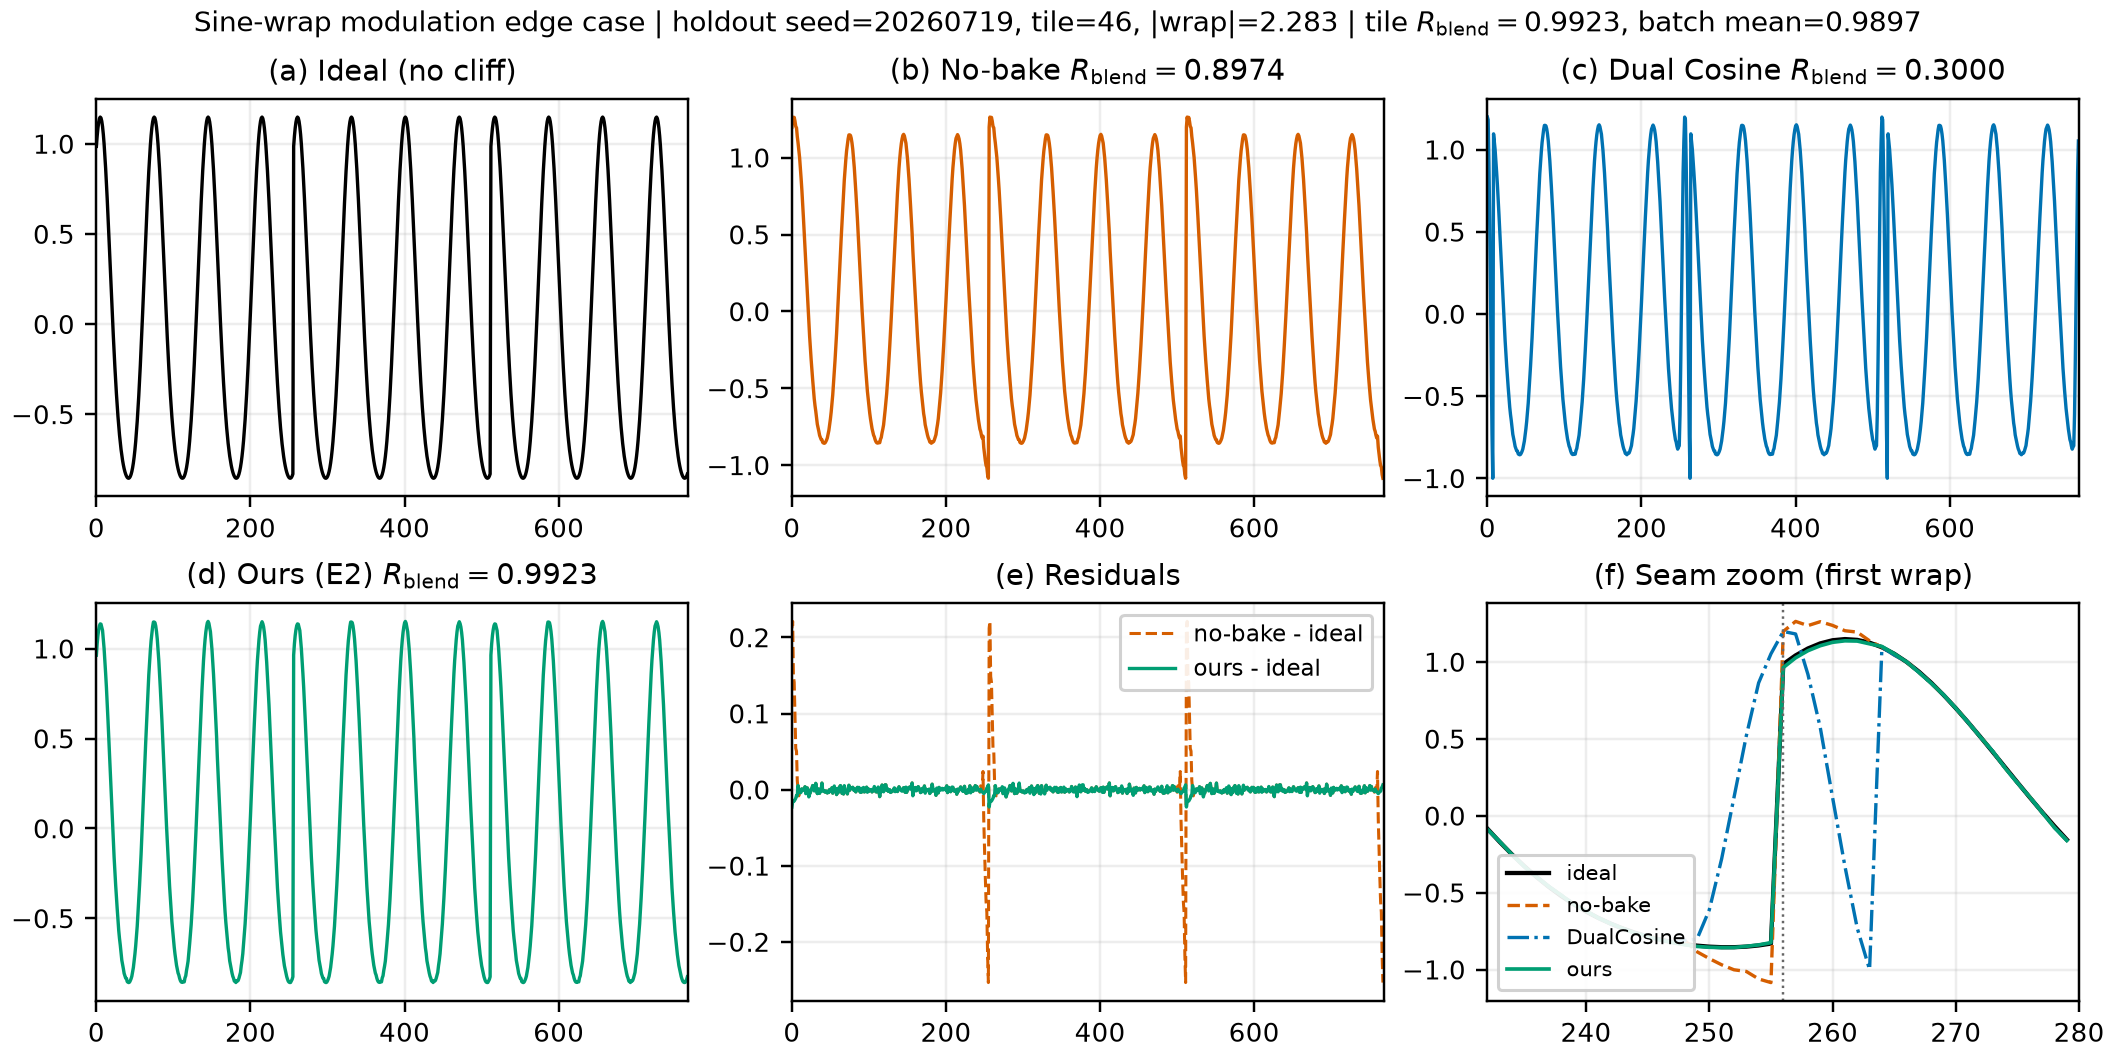
\includegraphics[width=\columnwidth]{figures/fig_intro_sine_problem.png}
  \caption{Hard sine-wrap holdout tile (seed~\texttt{20260719}).
  (a)~Ideal sibling $r^{\star}$.
  (b)~No-bake cracked engine.
  (c)~Dual Cosine fade.
  (d)~Ours (searched bake).
  (e)--(f)~Residual and seam zoom.
  Accompanying JSON scores use locked $R_{\mathrm{blend}}$ ($\alpha{=}0.7$; tile~46: no-bake $0.897$, Dual Cosine $0.300$, Ours $0.989$; Table~\ref{tab:n2n-vs-ours}).}
  \label{fig:intro-sine}
\end{figure}

Classical virtual-analog tools already address wrap energy locally
(BLIT/BLEP~\cite{stilson1996}, PolyBLEP~\cite{nam2009polyblep}, BLAMP~\cite{esqueda2016blamp}).
I score cycle-local bake versions of those operators beside Dual Cosine (Section~\ref{sec:va-seam-baselines}).
Label-free restoration such as Noise2Noise shows that useful reconstructors can be ranked without paired clean targets when the evaluation geometry is explicit~\cite{lehtinen2018,kashyap2021n2n}.
On the search side, I \emph{reuse} known NAS, aging evolution, PBT, CMA-ES, and PPO tools~\cite{elsken2019,real2019,jaderberg2017,schulman2017,khadka2018}: GA for diversity, PPO for discrete architecture edits, PBT-style exploit--mutate on elites.
The engineering choice is to combine them as an outer loop over compact seam-repair graphs; that combination is not claimed as an algorithmic contribution, and the $n{=}3$ outer-loop pilot serves solely as a compute-allocation heuristic rather than a confirmatory search-algorithm claim.

\paragraph{Key findings.}
Under the locked v10.1 $R_{\mathrm{blend}}$ protocol (objective wrap-discontinuity metrics only; no perceptual or listening claim, $N_{\mathrm{listeners}}{=}0$):
\begin{itemize}
  \item \textbf{Confirmatory (Holm--Bonferroni corrected, Table~\ref{tab:n2n-vs-ours}):} Converged DenoiseOpt beats matched \texttt{SeamN2N} on $10$-seed Holdout ($0.9903{\pm}0.0010$ vs $0.9764{\pm}0.0020$, $p_{\mathrm{adj}}{=}0.0039$), $10$-seed Multi-family ($0.9324{\pm}0.0038$ vs $0.9260{\pm}0.0031$, $p_{\mathrm{adj}}{=}0.0039$), and domain-searched vs domain-trained \texttt{SeamN2N} on disjoint $256$-cycle held-out splits for Factory+FX ($0.9108{\pm}0.0845$ vs $0.8772{\pm}0.1218$, $p_{\mathrm{adj}}{=}4.2{\times}10^{-15}$) and AKWF OA ($0.8740{\pm}0.1044$ vs $0.8009{\pm}0.1720$, $p_{\mathrm{adj}}{=}9.5{\times}10^{-21}$).
  \item \textbf{Hard cliffs \& perceptual/seam proxies:} On top-$10\%$ wrap cliffs, Dual Cosine collapses ($0.9913$ edge RMSE) while E2 plateau champions drop to $0.0086$--$0.0129$ vs $0.0203$ for \texttt{SeamN2N} (Table~\ref{tab:cliff-edge-rmse}), and $R_{\mathrm{blend}}$ tracks seam-local Edge RMSE ($\rho{=}{-}0.9737$, $p{<}10^{-300}$) and $>2$\,kHz click splatter ($\rho{=}{-}0.9342$, $p{<}10^{-300}$; Section~\ref{sec:proxy-and-lambda}).
\end{itemize}
\paragraph{Exploratory compute-allocation note.}
Under a $16$--$48$-step FitCell cap, the hybrid trails frozen Noise2Noise on $10$-seed holdout ($0.9710$ vs $0.9764$, $p{=}0.0020$); training to plateau (E2) reverses this gap.
An underpowered $n{=}3$ search-seed pilot ($0.9748{\pm}0.0018$, $p{=}0.25$, requiring $n{\ge}6$ seeds for $\alpha{=}0.05$) is used strictly as an exploratory compute-allocation heuristic rather than a confirmatory search-family claim (Section~\ref{sec:results}).
\paragraph{Scope and roadmap.}
Cycle-local wavetable seam repair for DSP and synthesis venues; formal wrap-closure proofs, search-convergence theorems, and human perceptual trials ($N_{\mathrm{listeners}}{=}0$) are out of scope (Section~\ref{sec:limitations}).
Section~\ref{sec:methods} defines $R_{\mathrm{blend}}$, $J$, and the operator space; Section~\ref{sec:experiments} details datasets and baselines; Section~\ref{sec:results} presents confirmatory, ablation, perceptual-proxy, and cross-domain/TDSE results.

\subsection{Contributions}
\label{sec:contributions}
\begin{enumerate}
  \item \textbf{Problem framing.} Wrap discontinuity as cycle-local seam restoration under tiled evaluation, with explicit $R_{\mathrm{seam}}$, $R_{\mathrm{body}}$, and primary locked $R_{\mathrm{blend}}$ ($\alpha{=}0.7$) plus latency-aware $J$.
  \item \textbf{Ideal-sibling protocol.} Unsupervised scoring via a procedural cliff-withheld twin plus mid-cycle engine identity, without paired studio-clean targets at search time.
  \item \textbf{Compact repair-operator space.} Searchable graphs over classical seam ops (DualCosine, FIR, VA residuals) and tiny residual nets (MLP/FIR/U-Net-lite/LSTM-lite/MoE), not end-to-end Demucs-scale stacks (Section~\ref{sec:bake}, Appendix~\ref{app:algorithms}).
  \item \textbf{Engineering instantiation (not an algorithmic claim).} DenoiseOpt reuses standard GA--PPO(+PBT) primitives as an outer loop over that operator space; an exploratory $n{=}3$ six-way $5$k pilot ($p{=}0.25$) serves solely as a compute-allocation heuristic for FitCell-to-plateau (Tables~\ref{tab:meta-approaches},~\ref{tab:v14-hybrid-converge}).
  \item \textbf{Open multi-seed, multi-family, and cross-domain evaluation.} Frozen \texttt{SeamN2N} and circular \texttt{SeamResUNet} neural baselines, $10$-seed holdout, multi-family, sawtooth/pulse, and wavetable-native boards, hard-cliff strata, $6$-seed Quantum Ring TDSE, and exploratory 2D/3D TDSE and 7-domain engineering transfer checks (Section~\ref{sec:ethics}, Appendix~\ref{app:transfer-bundle}).
\end{enumerate}
What is \emph{not} claimed as a contribution: a new foundational NAS/RL algorithm, formal wrap-closure theorems, or perceptual MOS/MUSHRA superiority.

\section{Related Work}
\label{sec:related_work}

I group prior work by mechanism.
\textbf{Used} citations ground methods I build on or compare against under my protocol.
\textbf{Screened} citations mark prior work I reviewed and ruled out (wrong domain, cost, or objective).
I cite those papers for positioning only.
They are not building blocks of DenoiseOpt.

\paragraph{Wavetable / virtual-analog foundations and discontinuity control.}
Foundational wavetable and virtual-analog (VA) oscillator work frames alias-free classic waveforms and wrap/corner discontinuities via BLIT/BLEP~\cite{stilson1996}, PolyBLEP~\cite{nam2009polyblep}, and BLAMP~\cite{esqueda2016blamp}.
Unlike runtime oversampled VA oscillators, cycle-local VA repair approximations (\texttt{PolyBLEP} $0.795$ $R_{\mathrm{blend}}$ at $0.87$\,ms, \texttt{BLAMP} $0.914$ at $20$\,ms, \texttt{BLIT/BLEP} $0.632$ at $71$\,ms on seed \texttt{20260719}; Table~\ref{tab:baselines-main}) either under-correct value jumps or incur high per-batch cost, whereas searched compact operators reach $0.9903$ at $1.03$\,ms/batch.
DDSP frames DSP modules as composable blocks~\cite{engel2020}.
I reuse that framing for small bake/FIR/MLP seam operators at cycle scale, rather than end-to-end vocoders.

\paragraph{Normalized cycle metrics.}
Audio restoration and synthesis surveys routinely rank models with SNR/SDR-style normalized errors on declared masks~\cite{purwins2019,stoller2018}.
My locked $R_{\mathrm{blend}}$ applies the same one-minus-relative-RMS clamp (Section~\ref{sec:residual-score}, Eq.~\eqref{eq:R-component}) separately on seam and body masks after tiling; it is a task-specific objective, not a perceptual score.

\paragraph{Label-free restoration.}
Noise2Noise learns restorers from corrupted observations alone~\cite{lehtinen2018,kashyap2021n2n}.
Mixture-invariant training ranks unsupervised systems without stem labels~\cite{wisdom2020}.
I train a corrupt-to-corrupt seam CNN on the same generator as the primary neural baseline (Section~\ref{sec:results}).
Full Demucs / DiffWave stacks are screened: domain and bake-budget mismatch~\cite{dfossez2019,kong2021}.

\paragraph{Compact waveform operators.}
Wave-U-Net, Conv-TasNet, dual-path, and attention audio models supply block priors I shrink to bake width~\cite{stoller2018,luo2019,luo2020dprnn,subakan2021,ronneberger2015,he2016resnet,vaswani2017}.
They supply block priors rather than serving as frozen full-scale separators inside every meta trial.

\paragraph{Search and hybrids.}
Neural architecture search (NAS) taxonomies, reinforcement-learning (RL) controllers, progressive and latency-aware NAS, aging evolution, population-based training (PBT), CMA-ES, and evolution-guided policy gradients motivate applying a hybrid outer loop to this DSP task~\cite{elsken2019,zoph2017nas,pham2018,liu2018pnas,tan2019mnasnet,real2019,jaderberg2017,hansen2016cmaes,khadka2018,schulman2017}.
Mixture-of-experts (MoE) soft gates motivate routing among small heterogeneous operators under one residual score~\cite{shazeer2017}.
Matched outer-loop bake-offs (Random, CMA-ES, REINFORCE, aging evolution, TPE vs hybrid) sit in Appendix~\ref{app:supplement}.
I do not claim a new foundational NAS/RL algorithm.

\paragraph{Used vs screened (short).}
Used anchors include VA discontinuity control~\cite{stilson1996,esqueda2016blamp,nam2009polyblep}, unsupervised restoration~\cite{lehtinen2018,kashyap2021n2n,wisdom2020}, DDSP~\cite{engel2020}, compact waveform operators as above, and NAS/RL/PPO/PBT/CMA-ES/ERL/MoE as above.
Screened as contrast only: MAML~\cite{finn2017}, DARTS~\cite{liu2019}, Demucs-scale enhancers~\cite{dfossez2019,dfossez2021}, DiffWave~\cite{kong2021}, and SEGAN-style full GAN loops~\cite{pascual2017}.
Claims stay inside cycle-local seam restoration under a declared compute budget.

\section{Methods}
\label{sec:methods}

\subsection{Notation}
\label{sec:notation}

Throughout, $x\in\mathbb{R}^{L}$ is the cracked single-period wavetable (engine input with open-wrap cliff).
Let $\mathcal{H}$ be the space of repair-operator configurations (discrete operator graph plus continuous bake parameters).
The \textbf{repair operator} $\Theta$ (legacy code: bake cell) is
\begin{equation}
\label{eq:Theta}
\Theta:\mathbb{R}^{L}\times\mathcal{H}\to\mathbb{R}^{L},\qquad
y=\Theta(x;h),\quad h\in\mathcal{H}.
\end{equation}
When continuous parameters alone are emphasized I write $\theta$ for the continuous slice of $h$ and $y=\Theta(x;\theta)$.
$r^{\star}\in\mathbb{R}^{L}$ is the procedural ideal sibling defined below.
Tiling length $N$ (typically $N{=}16$) forms $y_{\mathrm{tiled}}=\mathrm{Tile}(y,N)$ and $r^{\star}_{\mathrm{tiled}}=\mathrm{Tile}(r^{\star},N)$.
Seam width $W$ (code: \texttt{SEAM\_W}, typically $8$) is the neighborhood edited by classical fade and polish ops.
$R(a,b;\mathcal{M})$ is the masked unit-clamp score in~\eqref{eq:R-component} ($1$~=~best).
$R_{\mathrm{blend}}$ is the primary locked metric in~\eqref{eq:R-blend}.
\textbf{Prolonged $R$} tiles the whole cycle once (debug / superseded search key only; not used for Table~\ref{tab:n2n-vs-ours} or matched bake-off reporting).
These symbols follow a different convention from Noise2Noise clean/noisy pairs.

\begin{table}[t]
  \centering
  \caption{Core symbols used in Methods.}
  \label{tab:symbols}
  \setlength{\tabcolsep}{3pt}
  \begin{adjustbox}{max width=\columnwidth}
\begin{tabular}{@{}cl@{}}
    \toprule
    Symbol & Meaning \\
    \midrule
    $L$ & Cycle length (samples per period) \\
    $x$ & Cracked engine wavetable period (cliff on) \\
    $y=\Theta(x;h)$ & Baked cycle after seam ops / residual operator \\
    $\Theta$ & Repair operator (bake operator) $\mathbb{R}^{L}\times\mathcal{H}\to\mathbb{R}^{L}$ \\
    $h\in\mathcal{H}$ & Repair-operator configuration (ops + continuous $\theta$) \\
    $r^{\star}$ & Ideal sibling (same seed, cliff withheld) \\
    $G$ & Procedural period generator (cliff on/off) \\
    $N$ & Prolong tiling count \\
    $W$ & Seam neighborhood width \\
    $R(a,b;\mathcal{M})$ & Masked score; \emph{first} arg sets RMS denominator (Eq.~\eqref{eq:R-component}) \\
    $R_{\mathrm{seam}}$ & $R(r^{\star},y;\mathcal{S})$ (ideal vs repair at wrap) \\
    $R_{\mathrm{body}}$ & $R(x,y;\mathcal{B})$ (engine vs repair in mid-cycle) \\
    $R_{\mathrm{blend}}$ & $\alpha R_{\mathrm{seam}}+(1-\alpha)R_{\mathrm{body}}$, $\alpha{=}0.7$ (primary tables) \\
    Prolonged $R$ & Whole-cycle tiled debug score (superseded; ablation left column) \\
    $J$ & $R_{\mathrm{blend}}-\lambda\cdot\mathrm{latency\_norm}$ (outer selection) \\
    \bottomrule
  \end{tabular}
\end{adjustbox}
\end{table}

\subsection{Problem setup: cracked period and ideal sibling}
\label{sec:ideal-tile}

\textbf{Problem.} Given a cracked period $x$, choose a bake configuration $h$ so that the repaired cycle $y=\Theta(x;h)$ matches a no-cliff ideal under prolonged tiling.

\textbf{Ideal sibling and mid-cycle engine identity (explicit).}
Let $G(\mathrm{seed},\mathrm{cliff})$ denote the procedural generator used by the CUDA FitCell batch maker
(FitCell $=$ inner continuous-parameter fit of one candidate $\Theta$; Algorithm~\ref{alg:fit}):
one draw of frequency, phase, and mid-cycle content, with an optional open-wrap cliff of width $W$ at both ends.
For any seed,
\begin{equation}
\label{eq:G-siblings}
r^{\star}=G(\mathrm{seed},\,\mathrm{cliff{=}off}),\qquad
x=G(\mathrm{seed},\,\mathrm{cliff{=}on}).
\end{equation}
Thus $r^{\star}$ (ideal sibling) and $x$ (cracked engine) are \emph{paired twins of one procedural draw}:
same mid-cycle waveform content; they differ only by whether the wrap cliff (and engine-only seam-boosted noise) is applied.
\begin{itemize}
  \item $r^{\star}$ is a \textbf{scoring target only}. It is never emitted as a method output and is not a human-labeled clean stem.
  \item $x$ is the \textbf{operator input}. Repair $\Theta$ edits $x$ toward agreement with $r^{\star}$ at the seam and identity to $x$ in the mid-cycle body.
  \item Locked $R_{\mathrm{blend}}$ (Section~\ref{sec:residual-score}) combines $R_{\mathrm{seam}}=R(r^{\star},y;\mathcal{S})$ with $R_{\mathrm{body}}=R(x,y;\mathcal{B})$ at $\alpha{=}0.7$:
    seam fidelity to the cliff-withheld twin, plus mid-cycle identity to the cracked engine (so the bake cannot freely rewrite the period interior).
\end{itemize}
For an arbitrary cracked period from this family, the sibling is obtained by replaying the same seed with the cliff withheld
(that is the pair returned by \texttt{make\_batch}).
Here \emph{self-supervised via a procedural sibling} means: no human-labeled clean audio and no studio-clean targets enter the search loop.
Unlike Noise2Noise corrupt-to-corrupt training (\texttt{SeamN2N}, which sees only independent corrupted draws $x_1,x_2$), $r^{\star}$ provides exact cliff-free seam geometry for scoring without supplying perceptual ground truth~\cite{lehtinen2018,kashyap2021n2n}.

\begin{table}[t]
  \centering
  \caption{Consolidated metric role mapping.}
  \label{tab:metric-roles}
  \setlength{\tabcolsep}{4pt}
  \footnotesize
  \begin{tabular}{@{}lll@{}}
    \toprule
    Symbol & Definition & Role \\
    \midrule
    $1{-}R_{\mathrm{blend}}$ & $\alpha(1{-}R_{\mathrm{seam}}){+}(1{-}\alpha)(1{-}R_{\mathrm{body}})$ & Inner-loop FitCell training loss \\
    $R_{\mathrm{blend}}$ & $\alpha R_{\mathrm{seam}}{+}(1{-}\alpha)R_{\mathrm{body}}$ ($\alpha{=}0.7$) & Primary evaluation \& reporting \\
    $J$ & $R_{\mathrm{blend}}-\lambda\cdot\mathrm{latency\_norm}$ ($\lambda{=}0.02$) & Outer-loop champion selection \\
    $R_{\mathrm{prol}}$ & $R(r^{\star},y;\Omega)$ over full tiled $\Omega$ & Legacy debug only (unused in selection) \\
    \bottomrule
  \end{tabular}
\end{table}

\textbf{Worked example (Tile~46, Figure~\ref{fig:intro-sine}) and low-RMS edge case.}
On holdout Tile~46 (seed \texttt{20260719}), \texttt{no-bake} gives $(R_{\mathrm{seam}},R_{\mathrm{body}},R_{\mathrm{blend}})=(0.853,1.000,0.897)$, \texttt{DualCosine} collapses the seam $(0.000,1.000,0.300)$, \texttt{SeamN2N} reaches $(0.967,0.996,0.975)$, and \texttt{Ours E2} reaches $(0.989,0.999,0.992)$.
If an input's mid-cycle RMS approaches zero ($\mathrm{RMS}_{\mathcal{B}}(x)\to 0$), the denominator clamp $\epsilon{=}10^{-8}$ prevents division by zero and the $\max(0,\cdot)$ clamp keeps $R_{\mathrm{body}}\in[0,1]$, while $\alpha{=}0.7$ ensures seam errors still dominate $R_{\mathrm{blend}}$.

\subsection{Blended residual score and latency-aware objective}
\label{sec:residual-score}

\textbf{Primary metric.}
After tiling each period of length $L$ ($L{=}256$) $N$ times ($N{=}16$, total length $T{=}N L{=}4{,}096$), let $y$ be the repaired output, $r^{\star}$ the ideal sibling, and $x$ the cracked engine.
With seam half-width $W{=}8$, the wrap-neighborhood mask $\mathcal{S}$ and complementary mid-cycle body mask $\mathcal{B}$ are defined per tiled period $k\in\{0,\dots,N{-}1\}$ as
\begin{equation}
\label{eq:mask-SB}
\begin{aligned}
\mathcal{S} &= \bigcup_{k=0}^{N-1}\bigl([kL,\,kL{+}W)\cup[kL{+}L{-}W,\,(k{+}1)L)\bigr),\\
\mathcal{B} &= \bigcup_{k=0}^{N-1}[kL{+}W,\,kL{+}L{-}W) = \{0,\dots,T{-}1\}\setminus\mathcal{S}.
\end{aligned}
\end{equation}
By construction $\mathcal{S}\cap\mathcal{B}=\emptyset$ (zero overlap at every period boundary, $|\mathcal{S}|=2NW=256$ and $|\mathcal{B}|=N(L-2W)=3{,}840$), so $R_{\mathrm{body}}=R(x,y;\mathcal{B})$ never rewards leaving seam-adjacent samples unrepaired.
For masked sample set $\mathcal{M}\in\{\mathcal{S},\mathcal{B}\}$, let $|\mathcal{M}|$ be the number of scored samples and
\begin{equation}
\mathrm{RMS}_{\mathcal{M}}(u)=\sqrt{\frac{1}{|\mathcal{M}|}\sum_{i\in\mathcal{M}} u_i^2}.
\end{equation}
The implementation fixes $\varepsilon>0$ with $\varepsilon=10^{-6}$.
Component scores use the unit clamp (same normalized-error form as SNR-style objectives on a mask~\cite{purwins2019}):
\begin{equation}
\label{eq:R-component}
R(a,b;\mathcal{M})
=\mathrm{clamp}\!\left(
  1-\frac{\mathrm{RMS}_{\mathcal{M}}(a-b)}
         {\max\!\bigl(\mathrm{RMS}_{\mathcal{M}}(a),\,\varepsilon\bigr)},
  0,1\right).
\end{equation}
$R(a,b;\mathcal{M})\neq R(b,a;\mathcal{M})$ in general: the denominator uses the RMS of the \emph{first} argument only (ideal for $R_{\mathrm{seam}}$, engine for $R_{\mathrm{body}}$).
Then $R_{\mathrm{seam}}=R(r^{\star},y;\mathcal{S})$ (seam fidelity vs the ideal) and
$R_{\mathrm{body}}=R(x,y;\mathcal{B})$ (mid-cycle identity vs the engine).
The primary reported score is
\begin{equation}
\label{eq:R-blend}
\begin{aligned}
R_{\mathrm{blend}}
&=\alpha R_{\mathrm{seam}}+(1-\alpha)R_{\mathrm{body}},\\
\alpha&=0.7.
\end{aligned}
\end{equation}
Whole-curve prolonged $R$ is defined over the full tiled domain $\Omega{=}\{0,\dots,T{-}1\}$ as $R_{\mathrm{prol}}(r^{\star},y)=R(r^{\star},y;\Omega)$, which mixes seam repair with global waveform error; it is retained only as a superseded legacy key and never replaces $R_{\mathrm{blend}}$.
For real-world wavetable corpora without a procedural generator (Factory+FX and AKWF OA in Table~\ref{tab:n2n-vs-ours}), the self-supervised protocol instantiates $r^{\star}$ directly from unperturbed real cycles on a disjoint training split and injects a controlled wrap-cliff perturbation to form $x$, evaluating on held-out real cycles.

\textbf{Roles of the three quantities.}
\begin{center}
\small
\begin{adjustbox}{max width=\columnwidth}
\begin{tabular}{@{}lll@{}}
\toprule
Quantity & Role & Used for \\
\midrule
$R_{\mathrm{blend}}$ & Primary quality metric & Tables, figures, reporting \\
$J$ & Latency-aware search objective & Champion selection \\
N2N gate & Frozen neural benchmark & Holdout pass/fail \\
\bottomrule
\end{tabular}
\end{adjustbox}
\end{center}

\textbf{Search objective.}
Candidates maximize latency-aware
\begin{equation}
\label{eq:outer-obj}
\begin{aligned}
J&=R_{\mathrm{blend}}-\lambda\cdot\mathrm{latency\_norm},\\
\mathrm{latency\_norm}
&=\frac{\log(1+t_{\mathrm{ms}})}{\log(1+50)},
\quad \lambda=0.02.
\end{aligned}
\end{equation}
FitCell minimizes $1-R_{\mathrm{blend}}$. Selection and champion updates use $J$.
Here $\log(1+50)$ normalizes batch-64 CUDA runtime smoothly to $[0,1]$ against a $50$\,ms real-time bake ceiling (validated by the $\lambda\in[0,0.05]$ selection-invariance sweep in Section~\ref{sec:proxy-and-lambda}).
Using the fixed target $a$ ($r^{\star}$ for $R_{\mathrm{seam}}$, $x$ for $R_{\mathrm{body}}$) as the reference denominator in $R(a,b;\mathcal{M})$ follows standard normalized-error conventions~\cite{purwins2019} and agrees closely with symmetric normalization ($r{=}0.9988, \rho{=}0.9997$ in Section~\ref{sec:proxy-and-lambda}).
A champion must also strictly beat the frozen corrupt$\to$corrupt Noise2Noise holdout $R_{\mathrm{blend}}$ (primary baseline).

\textbf{Every} scored row applies some $\Theta$ to $x$ and is evaluated under~\eqref{eq:R-blend}.
The ideal sibling is the seam scoring target. Body identity uses the engine.

\begin{remark}[Noise2Noise primary baseline]
\label{rem:n2n}
\texttt{SeamN2N} (${\approx}53.5$k) is the primary neural comparator and champ gate.
Search may discover \texttt{n2n\_unet} operators at the same scale. TinyUNet1D \texttt{unet} is a different, smaller block~\cite{lehtinen2018,kashyap2021n2n}.
\end{remark}

\subsection{Seam bake operator and classical baselines}
\label{sec:bake}

A \textbf{repair operator} $\Theta(\cdot;h)$ composes classical seam ops (DualCosine, polish, soft seam, FIR blends) with optional tiny residual operators (MLP/FIR/U-Net-lite/attention-lite/LSTM-lite) and optional mixture-of-experts (MoE) soft gates over experts (Appendix~\ref{app:algorithms}, Algorithms~\ref{alg:dualcosine}--\ref{alg:moe}).
Bake parameters sit in a bounded box; architecture strings are discrete graphs over those ops.
Separate classical controls apply cycle-local BLIT/BLEP, PolyBLEP, and BLAMP residual corrections at the wrap on the cracked engine tile: they share the DualCosine / FIR interface and are not a full oscillator rewrite.
Roles in plain language: BLIT/BLEP and PolyBLEP correct a \emph{value} step at wrap, BLAMP corrects a \emph{slope}/corner jump, and DualCosine fades endpoints without a BLEP residual.
Section~\ref{sec:va-seam-baselines} scores them.

\paragraph{Four roles (keep separate).}
\label{sec:four-roles}
Four objects must stay distinct (Figure~\ref{fig:intro-sine}).
The \textbf{ideal sibling} $r^{\star}$ withholds the cliff and is a scoring target only (panel~(a)).
\textbf{No-bake} is the unrepaired passthrough $\Theta_{\mathrm{no\text{-}bake}}(x)=x$: the cracked engine scored against $r^{\star}$ (panel~(b)).
It leaves the engine unchanged and must not be confused with $r^{\star}$, residual-net skips, or learned identity maps.
\textbf{DualCosine} is the classical raised-cosine end fade on $x$ (panel~(c)).
It appears both as a classical board row and, separately, as a PPO advantage baseline (Remark~\ref{rem:dualcosine-centering}).
\textbf{Ours} is the searched bake $y=\Theta(x;h^{\star})$ from the hybrid outer loop (panel~(d)).

On mild cliffs, residual mass sits far below ideal RMS under the unit clamp of~\eqref{eq:R-blend}, so no-bake $R_{\mathrm{blend}}$ can look high even when the wrap click remains audible.
Treat that number as a do-nothing passthrough reference rather than a perceptual wrap-quality score.
Released JSON may still use the legacy key \texttt{identity} for no-bake.
Manuscript prose uses \emph{no-bake}.

\paragraph{Classical (non-AI) comparison board.}
\label{sec:classical-board}
Learned / searched methods are always ranked against the full classical board on $R_{\mathrm{blend}}$ (same $r^{\star}$):
no-bake, DualCosine / cosine fade, \texttt{seam\_fir3}, classic quadratic, hann/crossfade/soft fades, detrend/ensemble, poly seam, and cycle-local BLIT/BLEP / PolyBLEP / BLAMP where scored.
When tables show $\Delta R$ vs DualCosine, that is a reporting gap vs one classical bake, not the definition of reward.

\begin{remark}[DualCosine centering is PPO advantage only]
\label{rem:dualcosine-centering}
The outer objective remains~\eqref{eq:outer-obj}: maximize $R_{\mathrm{blend}}(r^{\star},x,y)$.
In the PPO branch only, I optionally form a centered advantage
\begin{equation}
\label{eq:dualcosine-centering}
\rho = R_{\mathrm{blend}} - R_{\mathrm{blend},\mathrm{DualCosine}},
\end{equation}
so early-search advantages are roughly zero-mean.
This does \emph{not} change selection, FitCell loss, champion ranking, or the matched $5$k meta-approach objective.
All of those still maximize $R_{\mathrm{blend}}$ (or $J$).
DualCosine centering is soft relative shaping for the actor--critic, not a hard absolute ranking target.
\end{remark}

\paragraph{Metric summary (search, selection, reporting, legacy).}
(1)~\textbf{FitCell loss:} $1 - R_{\mathrm{blend}}(r^{\star},x,y)$ with $\alpha{=}0.7$ and disjoint $\mathcal{S}/\mathcal{B}$ masks~\eqref{eq:mask-SB};
(2)~\textbf{Champion selection:} latency-aware $J = R_{\mathrm{blend}} - \lambda\cdot\mathrm{latency\_norm}$ ($\lambda{=}0.02$,~\eqref{eq:outer-obj});
(3)~\textbf{Primary reporting:} $R_{\mathrm{blend}}(r^{\star},x,y)$ on held-out seeds;
(4)~\textbf{Legacy debug score:} prolonged $R$ ($R_{\mathrm{prol}}$), retained only in historical search-trace artifacts and never used for primary selection or leaderboard reporting.

\subsection{Search pipeline}
\label{sec:pipeline-overview}

Figure~\ref{fig:denoiseopt-arch} summarizes the residual-scored hybrid loop.
Each outer iteration proposes a bake configuration $h$, runs FitCell (Appendix~\ref{app:algorithms}, Algorithm~\ref{alg:fit}) to fit continuous parameters under loss $1-R_{\mathrm{blend}}$, evaluates $R_{\mathrm{blend}}$ (and $J$) vs $r^{\star}$, and updates the population / PPO policy.

\paragraph{Main-text algorithm summary (before appendix listings).}
\begin{enumerate}
  \item \textbf{FitCell (inner):} Adam on $1-R_{\mathrm{blend}}$ over i.i.d.\ $G$ batches until relative residual change $<\varepsilon$ for patience $P$ steps, or hard cap $T_{\max}$ (Algorithm~\ref{alg:fit}).
  \item \textbf{GA branch:} tournament parents $\to$ crossover/mutate op graph $\to$ FitCell $\to$ insert by $J$ (Algorithm~\ref{alg:ga}).
  \item \textbf{PPO branch:} actor proposes discrete architecture edits; advantage uses optional DualCosine centering; clipped surrogate update (Algorithm~\ref{alg:ppo}); selection still maximizes absolute $R_{\mathrm{blend}}$/$J$.
  \item \textbf{PBT branch:} copy hyperparameters from elites into bottom quantile; multiplicative mutate; brief refit (Algorithm~\ref{alg:pbt}).
  \item \textbf{Hybrid rotation:} each outer step runs one or more of the above; champion is the best $J$ cell that also clears Dual Cosine and, when required, the N2N gate (Algorithm~\ref{alg:hybrid}).
\end{enumerate}
Full line-by-line pseudocode is in Algorithms~\ref{alg:ga}--\ref{alg:hybrid} (Appendix~\ref{app:algorithms}).

% DenoiseOpt overview architecture diagram (TikZ); placed before component deep-dives
\begin{figure}[t]
  \centering
  \resizebox{\columnwidth}{!}{%
  \begin{tikzpicture}[
    font=\footnotesize,
    box/.style={draw, rounded corners=1.5pt, align=center, inner sep=3pt, minimum height=0.55cm},
    io/.style={box, fill=black!6},
    classical/.style={box, fill=black!3},
    neural/.style={box, fill=black!8},
    meta/.style={box, fill=black!12},
    arr/.style={-{Stealth}, thick},
    node distance=0.42cm and 0.28cm
  ]
    % Top: generator siblings
    \node[io] (seed) {seed};
    \node[io, right=1.1cm of seed] (Goff) {$r^{\star}{=}G(\cdot,\mathrm{cliff\,off})$};
    \node[io, below=0.55cm of Goff] (Gon) {$x{=}G(\cdot,\mathrm{cliff\,on})$};

    % Middle: bake path
    \node[classical, right=0.85cm of Gon] (dc) {classical ops\\DualCosine / FIR};
    \node[neural, right=of dc] (cell) {repair operator $\Theta(x;h)$\\(+ residual / MoE)};
    \node[io, right=of cell] (y) {baked $y$};

    % Bottom: score + outer loop
    \node[meta, below=0.85cm of cell] (R) {$\max\,R_{\mathrm{blend}}(r^{\star},x,y)$\\(tile $N{=}16$)};
    \node[meta, below=0.5cm of R] (outer) {Hybrid outer loop:\\PPO $\cdot$ GA $\cdot$ PBT $\cdot$ NAS $\cdot$ combo};
    \node[io, right=0.55cm of outer] (champ) {Ours / champion $h^{\star}$};

    % Side labels for controls
    \node[classical, left=0.55cm of R, align=center] (nobake) {no-bake\\$\Theta{=}{\mathrm{id}}$};

    \draw[arr] (seed) -- (Goff);
    \draw[arr] (seed) |- (Gon);
    \draw[arr] (Gon) -- (dc);
    \draw[arr] (dc) -- (cell);
    \draw[arr] (cell) -- (y);
    \draw[arr] (y) |- (R);
    \draw[arr] (Goff) |- (R);
    \draw[arr, dashed] (Gon) |- (nobake);
    \draw[arr, dashed] (nobake) -- (R);
    \draw[arr] (R) -- (outer);
    \draw[arr] (outer) -- (champ);
    \draw[arr, dashed] (outer) |- ++(0,1.05) -| (cell);
  \end{tikzpicture}%
  }
  \caption{DenoiseOpt overview (before component deep-dives).
  Same-seed generator $G$ yields ideal sibling $r^{\star}$ (cliff off) and cracked engine $x$ (cliff on).
  Repair operator $\Theta(x;h)$ may include DualCosine/FIR and optional residual/MoE experts.
  No-bake is the identity control $x\mapsto x$.
  Selection objective is $J = R_{\mathrm{blend}} - \lambda\cdot\mathrm{latency\_norm}$ ($\lambda{=}0.02$).
  DualCosine centering (not shown) is PPO advantage shaping only.
  Dashed feedback: architecture proposals update the operator. Pseudocode in Appendix~\protect\ref{app:algorithms}.}
  \label{fig:denoiseopt-arch}
\end{figure}


\subsection{Search space and inner fit}
\label{sec:search-space}

Each genome encodes: ordered op list (fade, polish, FIR, pin, residual write), depth, residual operator type (none, MLP, FIR, U-Net-lite, attn-lite, LSTM-lite), optional MoE expert count $K\in\{2,3,4\}$, and continuous $\theta$ in the CUDA runner box bounds.
The searchable bake vocabulary includes a width-capped 1--2 layer LSTM block over the seam window or full cycle (distinct from the fixed supervised seq-LSTM SOTA baseline).
The live hybrid tag is \texttt{PPO+GA+PBT+NAS+depth+MoE} with LSTM enabled in the block graph.

FitCell draws sibling batches via $G$, applies $\Theta(\cdot;h)$, and steps Adam on $1-R_{\mathrm{blend}}$ until residual plateau or a searchable hard cap $T_{\max}$ (Algorithm~\ref{alg:fit}; default patience / $\varepsilon$ co-tuned online).
The short-cap D1 FitCell (${\approx}16$--$48$ steps) is retained only for the six-way matched bake-off; the hybrid-only follow-up uses the converge protocol (Section~\ref{sec:v14-converge}).

\subsection{Hybrid outer loop}
\label{sec:hybrid}

Each iteration rotates among branches: PPO, GA, PBT, NAS, and combo.
Selection and FitCell are always by absolute residual $R$ (maximize toward the ideal sibling, loss $1-R$).

\paragraph{Near-ceiling scores need reward shaping.}
\label{sec:reward-shaping}
On the sine{+}cliff generator, no-bake already sits near $R\approx 0.97$, and strong classical / searched bakes live in a narrow band toward $1$ (often $0.99$--$0.991$).
Absolute gaps of order $10^{-3}$--$10^{-2}$ are real but tiny as raw PPO/GA signals.
Without shaping, advantages collapse.
Hyperparameters (clip, entropy, mutation rate, population size, fit steps, learning rate) then decide whether the outer loop can climb the last percent.
I therefore treat reward shaping and search hyperparameters as first-class tunables alongside bake architecture.
In the present hybrid, PPO uses a searchable shaping mode among $\{\texttt{abs\_r},\,\texttt{vs\_dualcosine},\,\texttt{vs\_nobake},\,\texttt{neglog\_gap}\}$ (PBT-mutated, default $\rho = R - R_{\mathrm{DualCosine}}$ per Remark~\ref{rem:dualcosine-centering}).
PBT mutates fit / PPO hyperparameters and reward mode in-population. Plateau adaptation retunes branch mix and depth/MoE bias when champions stall.
The matched $5$k meta-approach comparison (Section~\ref{sec:meta-compare}) selects the outer-loop family under a shared short FitCell budget; the hybrid-only converge campaign then spends GPU on that winner.

\subsection{Meta-learning approach comparison}
\label{sec:meta-compare}

Beyond the hybrid outer loop, I compare five additional outer-loop families under a matched $5{,}000$-evaluation budget,
three search seeds (\texttt{1902771841}, \texttt{2026072701}, \texttt{2026072702}), and the same FitCell / $R_{\mathrm{blend}}{+}J$ protocol (LSTM and xLSTM included in the searchable bake vocabulary).
Table and figure legends use the short display names below. Artifact folders keep stable code keys (see the \codehref{https://github.com/reeldemo/denoise-opt}{nomenclature}):
\begin{itemize}
  \item \textbf{Random NAS} (\texttt{random}): independent uniform draws over bake graphs and fit hyperparameters (control).
  \item \textbf{Cont.\ CMA-ES} (\texttt{cmaes}): diagonal covariance-matrix adaptation over a continuous encoding of depth, width, operator kind, block logits, and fit hyperparameters~\cite{hansen2016cmaes}.
  \item \textbf{Arch REINFORCE} (\texttt{reinforce}): vanilla policy gradient over discrete architecture-edit actions (no clipped surrogate). Contrast to PPO~\cite{schulman2017,zoph2017nas}.
  \item \textbf{Aging evolution} (\texttt{aging\_evo}): regularized evolution with oldest-member replacement after tournament parent selection~\cite{real2017large,real2019}, distinct from the hybrid's non-aging tournament GA branch.
  \item \textbf{TPE Bayes NAS} (\texttt{tpe}): lightweight tree-structured Parzen estimator over discrete bake categoricals in the spirit of practical Bayesian optimization~\cite{snoek2012}.
\end{itemize}
I also run \textbf{Ours (hybrid GA--PPO)} (\texttt{hybrid\_lstm}): the multi-branch hybrid loop for $5{,}000$ evaluations with LSTM/xLSTM in the block vocabulary and online reward-mode / fit--PPO hyperparameter co-tuning, as the proposed matched-budget arm.
Results appear in Appendix~\ref{app:supplement} (Table~\ref{tab:meta-approaches}, Figures~\ref{fig:meta-approach-bars}--\ref{fig:meta-approach-compare}). Healed-sample overlays appear in Figure~\ref{fig:meta-heal-samples}.

\begin{remark}[Trial complexity]
\label{rem:complexity}
Per outer iteration the dominant cost is $O(T_{\mathrm{fit}}\cdot C_{\mathrm{fwd}})$ for fit steps times one forward bake.
Bake-width caps (tiny residual operators) keep $C_{\mathrm{fwd}}$ far below full-band Demucs/DiffWave forwards screened in Related Work.
\end{remark}

\subsection{Hyperparameters}
\label{sec:hyperparams}

Table~\ref{tab:hyperparams} lists the CUDA search defaults used for the $5$k-gate freeze reported in Results.
Under the near-ceiling residual regime (Section~\ref{sec:reward-shaping}), these outer-loop and fit hyperparameters are co-tuned with architecture. PBT and plateau adaptation continue to mutate several of them online.
Companion listings: Algorithms~\ref{alg:residual}--\ref{alg:hybrid} (Appendix~\ref{app:algorithms}).

\begin{table}[t]
  \centering
  \small
  \caption{Hybrid search hyperparameters (RTX~3090 DenoiseOpt CUDA search-runner defaults). Co-tuned with reward shaping under near-ceiling $R$ (Section~\ref{sec:reward-shaping}).}
  \label{tab:hyperparams}
  \setlength{\tabcolsep}{3pt}
  \begin{adjustbox}{max width=\columnwidth}
\begin{tabular}{@{}lp{0.48\columnwidth}@{}}
    \toprule
    Parameter & Value \\
    \midrule
    Population size $n$ & 12 \\
    GA tournament $k$ & 3 \\
    GA crossover fraction $p_c$ & $0.5$ (else clone elite parent) \\
    GA mutation & $\ge 1$ mutate after inherit ($+50\%$ second mutate) \\
    PPO clip $\epsilon$ & $0.2$ (default, searchable $\{0.1,0.2,0.25,0.3\}$) \\
    Adam learning rate (fit) & $3{\times}10^{-3}$ (default, PBT-searchable) \\
    Adam learning rate (policy) & $3{\times}10^{-4}$ \\
    Entropy coefficient (PPO) & $0.02$ (default, searchable $\approx 0.005$--$0.06$) \\
    PBT exploit / mutate & elite fraction $0.25$, multi-step arch+hp mutate \\
    MoE routing & \texttt{sequential} or \texttt{moe\_parallel} when enabled \\
    Plateau boredom threshold & $1000$ iters without champ improve \\
    E2 plateau stopping rule & $\text{rel.\ }\Delta R_{\mathrm{blend}}<10^{-4}$ for $\text{patience}{=}3$ steps, grad clip $1.0$ \\
    Cycle length $L$ / tiles $N$ / seam $W$ & $256$ / $16$ / $8$ \\
    Fit steps / batch (default) & $24$ / $48$ \\
    Algo tag & \texttt{PPO+GA+PBT+NAS+depth+MoE} \\
    \bottomrule
  \end{tabular}
\end{adjustbox}
\end{table}

\section{Experiments}
\label{sec:experiments}

\paragraph{Evaluation protocol (locked).}
\label{sec:eval-protocol}
All primary tables use the same locked residual.
Given a cracked engine tile $x\in\mathbb{R}^{L}$ and its cliff-withheld ideal sibling $r^{\star}\in\mathbb{R}^{L}$ (generated directly from the underlying continuous oscillator prior to injecting the wrap-cliff offset and end-noise, using holdout PRNG seeds \texttt{20260719}--\texttt{20260728} strictly disjoint from search seeds \texttt{1902771841}, \texttt{2026072701}, \texttt{2026072702} so no FitCell gradient or search selection ever sees evaluation tiles),
prolong each cycle $N{=}16$ times, form wrap neighborhoods of width $W{=}8$ at every period head/tail,
and compute $R_{\mathrm{seam}}=R(r^{\star},y;\mathcal{S})$ and $R_{\mathrm{body}}=R(x,y;\mathcal{B})$ via~\eqref{eq:R-component} with $\varepsilon=10^{-6}$, then
\[
R_{\mathrm{blend}}=\alpha R_{\mathrm{seam}}+(1-\alpha)R_{\mathrm{body}},\qquad\alpha{=}0.7.
\]
Body residual uses the engine $x$ as the first argument so mid-cycle identity is rewarded; swapping arguments changes the score.
No per-table rescaling: reported scores are that clamp in $[0,1]$.
Search maximizes
$J=R_{\mathrm{blend}}-\lambda\cdot\mathrm{latency\_norm}$ with $\lambda{=}0.02$ and
$\mathrm{latency\_norm}=\log(1{+}t_{\mathrm{ms}})/\log(1{+}50)$.
Frozen Noise2Noise corrupt$\to$corrupt holdout $R_{\mathrm{blend}}$ serves as the neural gate: short-FitCell hybrid search clears Dual Cosine but sits below this gate, whereas FitCell-to-plateau clears it across all three tested search seeds (Section~\ref{sec:results}).
Secondary keys (SNR, SDR, wrap-jump, seam-local edge RMSE) are reported where tabulated;
whole-curve prolonged $R$ is debug-only and never used for selection.
PESQ/STOI/MUSHRA are out of scope on non-speech cycles ($N_{\mathrm{listeners}}{=}0$).

\paragraph{Which numbers are multi-seed.}
Holdout / multi-family means are mean$\pm$std over five evaluation seeds (\texttt{20260719}--\texttt{20260723}), extended to ten evaluation seeds (\texttt{20260719}--\texttt{20260728}) in the released artifacts.
Matched-$5$k ($5{,}000$-evaluation) outer-loop bake-off means are mean$\pm$std over $n{=}3$ pilot search seeds (\texttt{1902771841}, \texttt{2026072701}, \texttt{2026072702}), supplemented by two extra search seeds (\texttt{2026072703}, \texttt{2026072704}) and a three-seed $5$k branch ablation.
The FitCell-to-plateau follow-up (Section~\ref{sec:v14-converge}) reports both the single-seed in-loop freeze (\texttt{1902771841}) and three-seed holdout replication.
N2N train seed is \texttt{424242}.
Transfer Table~\ref{tab:transfer-main} is one domain-trained hybrid per board (search seed \texttt{1902771841}), not multi-seed averages.
I report the hybrid\_lstm freeze plus holdout / multi-family / Factory+FX / AKWF / transfer benches.
Venue: DSP / synthesis artifact repair (DAFx / AES / arXiv cs.SD).

\paragraph{Statistical reporting (what I compute).}
Unless a table caption says otherwise, multi-seed cells are arithmetic mean$\pm$sample std over the named seed list (not Gaussian confidence intervals).
Paired holdout comparisons test the null hypothesis $H_0{:}\,\mathbb{E}[\Delta]{=}0$ on identical paired seed lists ($n{=}5$ or $n{=}10$ evaluation seeds) using both a two-sided exact binomial sign test on win counts and a two-sided exact sign-flip permutation test (enumerating all $2^n$ sign assignments on per-seed deltas $\Delta_i$, giving minimum attainable $p{=}2/2^n$: $0.0625$ at $n{=}5$ and $0.0020$ at $n{=}10$), alongside $10{,}000$-resample paired bootstrap 95\% CIs and Hedges $g_z$ in Appendix~\ref{app:secondary-results}.
All primary four-board comparisons in Table~\ref{tab:n2n-vs-ours} apply Holm--Bonferroni multiple-testing correction ($p_{\mathrm{adj}}{\le}0.0039$ across all four boards); small-$n{=}3$ outer-loop pilot checks remain unadjusted exploratory diagnostics.
Search hyperparameters (learning rates, population sizes, mutation rates, and FitCell steps) are listed in Table~\ref{tab:hyperparams}.
Win/loss \emph{counts} at small $n$ also report Wilson 95\% score intervals for the win proportion (e.g.\ 10/20 board wins $\Rightarrow$ CI $[0.30,0.70]$).
Paired multi-family comparisons use a two-sided sign test on per-board mean deltas (reported $p$ values; $p{=}1.0$ means parity, not overlap-driven superiority).
Matched-$5$k outer-loop comparisons use paired deltas across three search seeds per family; with $n{=}3$, two-sided sign-flip tests cannot reach $p<0.25$ when all deltas share sign, treat Table~\ref{tab:meta-approaches} as descriptive selection, not inferential ranking.
I do \emph{not} run ANOVA across outer-loop families beyond mean$\pm$std in Table~\ref{tab:meta-approaches}, and I do not invent MOS confidence intervals.
Scope: this is a technical investigation, not a human listening trial ($N_{\mathrm{listeners}}{=}0$; no preference rates).
Reproducibility: all primary tables, statistical tests, and figures reproduce from the unified repository (\codeurl{https://github.com/reeldemo/denoise-opt}, RTX~3090, CUDA, PyTorch) via the repository's evaluation, domain-search, and plotting scripts.

\paragraph{Experimental setup (datasets, compute).}
\begin{itemize}
  \item \textbf{Primary procedural datasets.} Generator $G$: $L{=}256$ two-harmonic sine{+}cliff; seam width $W{=}8$; cliff amplitude $\pm\mathcal{U}(0.08,0.43)$; FitCell/search draws i.i.d.; frozen holdout metrics draw $n{=}4096$ (seed \texttt{20260719}) plus five-seed score batches (\texttt{20260719}--\texttt{20260723}).
    Multi-family SOTA: $10$ families $\times$ $2$ seeds $\times$ batch $64$ ($n{=}1280$).
    Factory+FX / AKWF wavetable-native boards: $n{=}1280$ each (ReelSynth exports; AKWF CC0).
  \item \textbf{Transfer stress boards.} Seven wrap-protocol boards ($n{=}256$ each); full protocol and tables in Appendix~\ref{app:transfer-bundle}.
  \item \textbf{FitCell / outer loop.} Adam on $1-R_{\mathrm{blend}}$; D1 short cap ${\approx}16$--$48$ steps; converge campaign searchable patience/$\varepsilon$/$T_{\max}\!\in\!\{512,\ldots,2048\}$, batch ${\approx}96$, two sequential proposals/iter (Section~\ref{sec:pipeline-overview}).
    Matched $5$k evals: Random, CMA-ES, REINFORCE, Aging, TPE, hybrid (3 search seeds).
    Hybrid-only FitCell-to-plateau: $750$ outer iters, seed \texttt{1902771841} (${\approx}46.9$\,h wall).
  \item \textbf{Baselines.} no-bake, DualCosine, FIR/endpoint classical board, SeamN2N (${\approx}53.5$k, $4000$ Adam steps, train seed \texttt{424242}), VA residuals where scored.
  \item \textbf{Compute.} Single NVIDIA GeForce RTX~3090 ($24$\,GB); host desktop Windows; Python~$3.12$, PyTorch~$2.6$+CUDA~$12.4$; no multi-GPU.
    Historical prolonged-$R$ $5$k-style freeze ${\approx}7.9$\,h (Table~\ref{tab:compute}); D1 hybrid mean wall ${\approx}8.4$\,h/seed.
  \item \textbf{Artifacts.} Frozen JSON matrices and figure sources ship in the paper repository (Section~\ref{sec:ethics}).
\end{itemize}

\subsection{Dataset}
\label{sec:dataset}

\paragraph{Creation.}
The paper-facing evaluation corpus is a frozen draw from the same synthetic generator used by the CUDA search runner (\texttt{make\_batch}).
Cycles are length $L{=}256$.
A two-harmonic sine is drawn with frequency $\sim\mathcal{U}(1,4)$ and phase $\sim\mathcal{U}(0,2\pi)$, then an open-wrap seam cliff of amplitude $\pm\mathcal{U}(0.08,0.43)$ is applied over $\texttt{SEAM\_W}{=}8$ samples at both ends.
Seam-boosted Gaussian noise (scale $0.02$ at the ends, $0.15\times$ in the mid-cycle) forms the engine input.
The ideal withholds the cliff and serves only as scoring target $r^{\star}$, never as a method output, while no-bake leaves the cracked engine unchanged and scores that unrepaired $x$ against the same $r^{\star}$.
Prolonged residual $R$ tiles each cycle $N{=}16$ times before the RMS ratio.
Holdout seed \texttt{20260719} is distinct from hybrid search seed \texttt{1902771841}.
The search campaign draws fresh i.i.d.\ batches from this generator and never trains on the frozen holdout tensors: there is no supervised clean/noisy training split of studio audio.

\paragraph{Multi-family diversity ($\ge 20$ waveforms).}
Beyond the single sine{+}cliff holdout, Phase~3a scores methods on \textbf{20} generative draws: ten family variants (\texttt{sine\_cliff}, \texttt{harmonic\_fft}, \texttt{am\_fm}, \texttt{nonlinear}, \texttt{combo}, \texttt{triple\_mix}, \texttt{extreme\_overlay}, \texttt{open\_wrap\_bias}, \texttt{soft\_noise}, \texttt{wide\_seam}) $\times$ two seeds (\texttt{20260719} and \texttt{20260720}), batch 64 each ($128$ cycles per family, $1{,}280$ total).
These Python generative variants stress harmonic / AM--FM / nonlinear / overlay / open-wrap behavior of \texttt{make\_batch} and remain the primary SOTA matrix.
Separately, \texttt{export\_sound\_bench\_tiles} exports \textbf{20} Rust \texttt{sound\_bench} engine/ideal pairs (10 families $\times$ 2 seeds, $L{=}256$, byte-aligned with \texttt{generate\_sound} / \texttt{generate\_sound\_ideal}) scored under the same residual geometry as a secondary transfer block (Table~\ref{tab:rust-bench}).
Every method sees the same tensors per waveform.
\textbf{Primary classical comparison} is absolute $R_{\mathrm{blend}}$ against the non-AI board (no-bake, DualCosine, \texttt{seam\_fir3}, poly, fades, VA residuals, Section~\ref{sec:classical-board}).
The search objective is maximize $R$ toward the ideal sibling (best $R{=}1$).
DualCosine is one classical comparator and a PPO centering constant.
It is not the reward target.

\paragraph{Dataset statistics.}
Table~\ref{tab:dataset-stats} and Figure~\ref{fig:dataset-size} inventory primary evaluation boards; transfer sizes are in Appendix~\ref{app:transfer-bundle}.
The primary procedural holdout is a frozen $4{,}096$-cycle metrics draw ($L{=}256$, $N{=}16$ tiles, seed \texttt{20260719}) plus a matched score batch of $64$ cycles (five consecutive seeds for classical mean$\pm$std).
Multi-family SOTA scores $20$ waveforms ($10$ families $\times$ $2$ seeds, batch $64$, $1{,}280$ cycles).
Wavetable-native boards use ReelSynth Factory+FX exports ($n{=}1{,}280$: $640$ dry + $640$ FX) and AKWF CC0 cycles ($n{=}1{,}280$) so Plot~4 corpus bars are comparable to multi-family ($1{,}280$).
Sci/eng transfer tiles ($1{,}536$ periods total) are summarized in Appendix~\ref{app:transfer-bundle}.
Search never trains on the frozen holdout. N2N/seq baselines use disjoint train seeds \texttt{424242}/\texttt{424243}.
Artifacts: \codehref{https://github.com/reeldemo/denoise-opt}{dataset artifacts}.

\begin{table}[htbp]
  \centering
  \caption{Dataset statistics (evaluation boards).
    $L{=}256$ unless noted. Hours are raw source duration on disk where measurable, not tiled period count.
    Plot~4 compares ${\approx}1{,}280$-height boards only (multi-family / Factory+FX / AKWF / transfer).}
  \label{tab:dataset-stats}
  \setlength{\tabcolsep}{3pt}
  \begin{adjustbox}{max width=\columnwidth}
\begin{tabular}{@{}llp{0.42\columnwidth}@{}}
    \toprule
    Board & Size & Notes \\
    \midrule
    Holdout metrics & $4{,}096$ cycles & seed \texttt{20260719}, $N{=}16$ tiles \\
    Score batch & $64$ cycles & classical / favorite tables \\
    Multi-family SOTA & $1{,}280$ cycles & $10$ families $\times$ $2$ seeds $\times$ $64$ \\
    Factory+FX export & $1{,}280$ periods & $640$ dry + $640$ FX mid-tile extracts \\
    AKWF OA & $1{,}280$ periods & CC0 single-cycle WAVs \\
    Meta hybrid\_lstm & $1{,}200$ iters & $R_{\mathrm{blend}}{+}J$, seed \texttt{1902771841} \\
    CWRU & $256$ periods & $4$ MAT files, DE @12\,kHz \\
    MFPT & $256$ periods & shaft-rate windows \\
    MIT-BIH & $256$ periods & $10$ records @360\,Hz \\
    PTB-XL subset & $256$ periods & $94$ \texttt{*\_hr} @500\,Hz \\
    synth CNC / PMU & $256{+}256$ & procedural pilots \\
    \bottomrule
  \end{tabular}
\end{adjustbox}
\end{table}

\begin{figure}[t]
  \centering
  \includegraphics[width=\columnwidth]{figures/fig_dataset_size_overview.png}
  \caption{Corpus sizes across evaluation boards (cycles or periods).
    Holdout metrics draw, matched score batch, multi-family SOTA, factory/AKWF wavetable-native sets, and summed transfer periods.}
  \label{fig:dataset-size}
\end{figure}

\paragraph{Dataset metrics.}
A metrics draw of $4{,}096$ cycles under the holdout seed yields mean ideal RMS $0.721\pm0.016$, mean engine residual RMS $0.021\pm0.013$, and mean absolute wrap jump $|x_0-x_{L-1}|$ of $0.913\pm0.634$.
No-bake (passthrough) on that draw scores mean $R\approx0.971$.
Method tables use a matched score batch of $64$ cycles from the same seed (the \codehref{https://github.com/reeldemo/denoise-opt}{canonical evaluation tensors}), five consecutive seeds for mean$\pm$std on the classical table, and the 20-waveform matrix for SOTA secondary metrics.
Figure~\ref{fig:dataset-distributions} summarizes the $4{,}096$-cycle metrics draw: ideal RMS clusters near $0.72$, wrap jumps span nearly three orders of magnitude (median $\approx 0.83$), and no-bake $R$ is high on easy tiles but falls below $0.91$ on the hardest decile of wrap jumps.
Figure~\ref{fig:intro-sine} is the documented sine-wrap edge case: a high-$|wrap|$ holdout tile where cliff modulation is visible, scored with DualCosine and the top neural favorite under the same residual $R$ (tile $R\approx0.9917$, favorite batch mean $R\approx0.991$).

\begin{figure}[t]
  \centering
  \includegraphics[width=\columnwidth]{figures/fig_dataset_distributions.png}
  \caption{Holdout distribution statistics (seed \texttt{20260719}, $n{=}4{,}096$ cycles).
    Distinguish: ideal sibling $r^{\star}$ (cliff withheld), no-bake $=$ unrepaired cracked engine (not $r^{\star}$), and DualCosine $=$ one classical bake.
    Top left: ideal RMS per cycle.
    Top right: engine residual RMS before any bake.
    Bottom left: wrap jump magnitude $|x_0-x_{L-1}|$ (cliff hardness proxy).
    Bottom right: no-bake prolonged $R$ (passthrough, $x\mapsto x$).
    Dashed and dotted vertical lines mark mean and median.
    Hard-cliff reporting (Section~\ref{sec:results}) uses the top 10\% wrap-jump stratum where no-bake $R$ drops.}
  \label{fig:dataset-distributions}
\end{figure}

\paragraph{Inference, classical, and learned baselines.}
High-$R$ fitted operators ($R\ge 0.98$) are timed on CUDA (batch 64, prolonged residual).
Ten non-learnable bake denoisers share the frozen canonical holdout against the neural favorite (Table~\ref{tab:canonical-methods}).
Cycle-local BLIT/BLEP, PolyBLEP, and BLAMP seam repairs are scored on the same holdout / cliff / multi-family protocol (Table~\ref{tab:va-seam-blep} and the \codehref{https://github.com/reeldemo/denoise-opt}{VA results}) and illustrated on the intro high-wrap tile (Figure~\ref{fig:va-seam-techniques}).
Fixed-arch MLP-on-$R$ and CNN/U-Net-lite-on-$R$ baselines (no outer NAS) are trained on $1{-}R$ with the same generator and scored in the SOTA matrix.
Phase~B adds a primary corrupt$\to$corrupt Noise2Noise seam CNN (train seed \texttt{424242}, disjoint from holdout), a secondary sibling-supervised ceiling on the same architecture, and lightweight LSTM / depthwise 1D-CNN seq restorers (train seed \texttt{424243}).
No search-champion weights initialize those baselines.
Family-conditional hardness uses the separate Rust procedural $100{,}000$-cycle bench reported in Results.

\paragraph{Cliff strata and wavetable-native realism.}
A $4{,}096$-tile holdout draw (seed \texttt{20260719}) is stratified by engine wrap-jump percentiles (top 25\% / top 10\%), with cutoffs in the \codehref{https://github.com/reeldemo/denoise-opt}{cliff-strata data}.
Hard-cliff is the operative regime for claims about DualCosine collapse vs favorite retention.
Edge RMSE is the locked required seam-local secondary. Click energy is optional.
Wavetable-native transfer (Phase~F1) scores true ReelSynth-exported factory periods (primary) and external AKWF CC0 WAVs (secondary) under the same close-seam$\to$open-wrap protocol.
Procedural stand-ins are tertiary smoke only.
Speech/music LibriSpeech/MUSDB corpora remain off.
% Short Experiments note for hear pack + vibrato.
% Included from experiments.tex.

\paragraph{Audible demos and vibrato spectrograms.}
Downloadable clips (no-bake / DualCosine / Ours, $44.1$\,kHz mono, A4, $3$\,s):
\href{https://github.com/reeldemo/denoise-opt}{hear-sample WAVs}
($n{=}5$ tiles $\times$ $3$ methods $=15$ WAVs).
Rebuild script:
\href{https://github.com/reeldemo/denoise-opt}{the repository script}.
Slow-vibrato spectrogram protocol
(\href{https://github.com/reeldemo/denoise-opt}{the repository script},
artifacts:
\href{https://github.com/reeldemo/denoise-opt}{vibrato folder})
scores the same bake operators under modulated-pitch playback. Figures appear in Section~\ref{sec:vibrato-eval}.
These assets support informal audition only.
\textbf{Listening statistics:} $N_{\mathrm{listeners}}{=}0$; no MOS, MUSHRA, forced-choice A/B rates, or significance tests are reported (and none are invented).
Objective companions are cycle-local / prolonged $R$ on the same tiles.
The planned listening protocol (if run later) is in Section~\ref{sec:listening-protocol}.


\paragraph{Compute budget (matched reporting).}
Table~\ref{tab:compute-n2n-hybrid} compares evaluation counts and logged GPU wall time for Noise2Noise vs hybrid search.
Hybrid search spends many more outer evaluations than the one-shot N2N trainer; Table~\ref{tab:compute-n2n-hybrid} includes the three-seed plateau replication and ten-seed holdout re-score.

\begin{table}[t]
  \centering
  \caption{Compute comparison (single GPU per row; GPU model from run metadata).
    \textbf{Evaluations} counts outer-loop architecture proposals for hybrid search, or Adam steps for the one-shot Noise2Noise trainer.
    Matched-$5$k historical freeze used RTX~3090; N2N retrain, FitCell-to-plateau, and holdout re-scores used RTX~3060 (Section~\ref{sec:experiments}).
    $5{,}000$ is the stopping gate on outer iterations; $\approx 6{,}922$ counts clean architecture evaluations in the archived trace when every proposal was scored.
    Noise2Noise gate $R_{\mathrm{blend}}$ is on the frozen holdout (eval seed \texttt{20260719}).}
  \label{tab:compute-n2n-hybrid}
  \setlength{\tabcolsep}{3pt}
  \footnotesize
  \begin{adjustbox}{max width=\columnwidth}
  \begin{tabular}{@{}lp{0.34\columnwidth}rr@{}}
    \toprule
    Method & Protocol & Evaluations & GPU-h \\
    \midrule
    SeamN2N (corrupt$\to$corrupt) & One training run; holdout eval & $20{,}000$ steps & ${\approx}0.043$ \\
    Hybrid (matched D1) & Outer loop; 3 search seeds & $5{,}000$/seed & ${\approx}8.4$ mean \\
    Hybrid FitCell-to-plateau (Seed 1) & Outer loop; search seed \texttt{1902771841} & $750/750$ & ${\approx}46.9$ \\
    Multi-seed plateau (Seeds 2 \& 3) & Seeds \texttt{2026072701}/\texttt{02} & $750$/seed & ${\approx}36.0$ / ${\approx}47.9$ \\
    Ten-seed holdout re-score & Eval seeds \texttt{20260719}--\texttt{28} ($n{=}10$) & 10 seeds $\times$ 4 methods & ${\approx}0.05$ \\
    \bottomrule
  \end{tabular}
  \end{adjustbox}\\[0.35em]
  {\footnotesize SeamN2N wall time is $155.2$\,s from the N2N baseline log.
  Matched-$5$k mean wall from Table~\ref{tab:meta-approaches}.
  Plateau wall from Section~\ref{sec:v14-converge}.}
\end{table}


\section{Results}
\label{sec:results}

This section reports objective wrap-repair scores under locked $R_{\mathrm{blend}}$
(Sections~\ref{sec:v10-freeze}--\ref{sec:n2n-vs-ours-boards}).
Higher is better. Unless noted, multi-seed cells are mean$\pm$std.
Appendix~\ref{app:supplement} holds the matched outer-loop bake-off, ablations, HP probes, and transfer latency.
Limitations are collected in Section~\ref{sec:limitations}.
The evaluation protocol is stated in Section~\ref{sec:experiments}.

\paragraph{How to read the main numbers.}
\begin{enumerate}
  \item \textbf{Holdout vs Noise2Noise and Dual Cosine} (Table~\ref{tab:n2n-vs-ours}):
    short-FitCell hybrid is close to, but below, Noise2Noise, and far above Dual Cosine.
  \item \textbf{Which outer loop to keep} (Table~\ref{tab:meta-approaches}):
    hybrid has the top descriptive mean in a matched $5$k bake-off ($n{=}3$ search seeds; vs runner-up mean $\Delta{=}{+}0.0114$, bootstrap CI $[0.0064,0.0144]$, $p{=}0.25$; Appendix~\ref{sec:meta-approaches-results}), compute allocation only, not outer-loop superiority.
  \item \textbf{Longer FitCell} (Table~\ref{tab:v14-hybrid-converge}):
    seed \texttt{1902771841} logs in-loop $R_{\mathrm{blend}}{\approx}0.9912$, and three-seed holdout replication reaches $0.9881{\pm}0.0029$ vs Noise2Noise gate $0.9766$ ($3/3$ wins, $p{=}0.25$ at $n{=}3$).
  \item \textbf{Where classical fails} (Section~\ref{sec:cliff-strata}):
    hard wrap cliffs collapse Dual Cosine; searched operators and Noise2Noise hold.
\end{enumerate}

\begin{figure}[t]
  \centering
  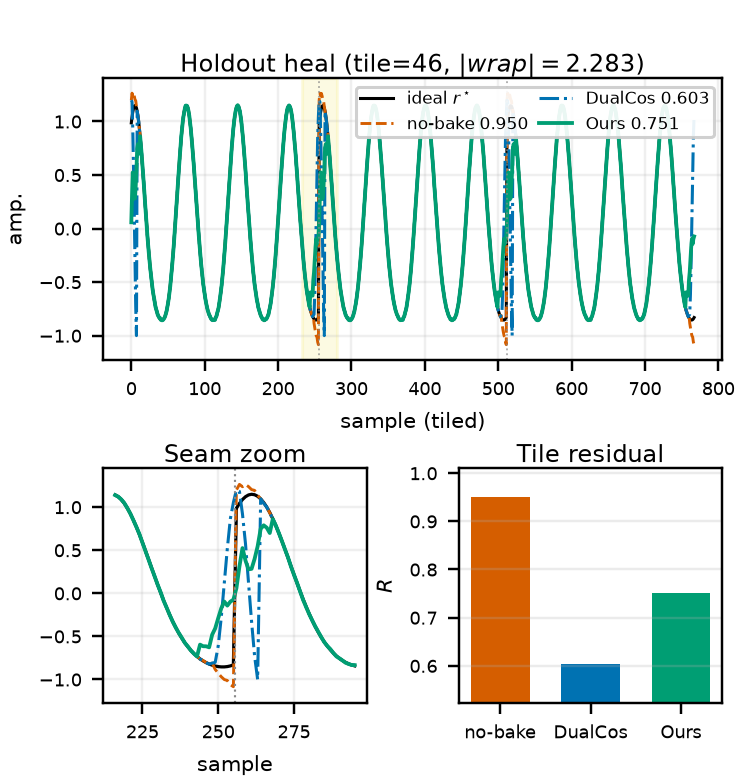
\includegraphics[width=\columnwidth]{figures/fig_meta_heal_samples.png}
  \caption{Holdout wrap-seam heal for the FitCell-to-plateau hybrid champion (in-loop $R_{\mathrm{blend}}{\approx}0.9912$, search seed \texttt{1902771841}; three-seed holdout mean $0.9881{\pm}0.0029$) vs no-bake, Dual Cosine, and ideal sibling $r^{\star}$.}
  \label{fig:meta-heal-samples}
\end{figure}

\subsection{A short hybrid search under $R_{\mathrm{blend}}$}
\label{sec:v10-freeze}

I first ask whether a hybrid GA+PPO search can beat frozen Noise2Noise under $R_{\mathrm{blend}}$ and $J$.
A $1{,}200$-iteration run (seed \texttt{1902771841}, ${\approx}1.65$\,h) selects on $J$~\eqref{eq:outer-obj} with $\lambda{=}0.02$.
The champion reaches $R_{\mathrm{blend}}{\approx}0.9695$ ($J{\approx}0.9603$, $t{\approx}5.08$\,ms).
Dual Cosine on the same runner scores ${\approx}0.504$.
The frozen Noise2Noise holdout gate is ${\approx}0.9750$.
So this short search clears Dual Cosine but not Noise2Noise.
Artifacts:
\codehref{https://github.com/reeldemo/denoise-opt}{hybrid search data}.

\subsection{Noise2Noise vs Ours on four boards}
\label{sec:n2n-vs-ours-boards}

Table~\ref{tab:n2n-vs-ours} is the main comparison under locked $R_{\mathrm{blend}}$.
Dual Cosine is the classical fade on every board.
Noise2Noise is the primary neural gate for this protocol (not a DenoiseOpt variant).

\paragraph{Holdout.}
In the earlier five-seed pilot (\texttt{20260719}--\texttt{20260723}), table means are
$0.9767{\pm}0.0015$ (Noise2Noise) vs $0.9708{\pm}0.0014$ (short-FitCell hybrid).
Those $\pm$ values are sample std over seeds, not confidence intervals; the bands can overlap even when one method leads on every draw.
Paired per-seed holdout scores give mean $\Delta R_{\mathrm{blend}}$ (Ours$-$N2N) $={-}0.0059$ with Noise2Noise strictly higher on all five seeds (two-sided sign test $p{=}0.062$, $n{=}5$).
Dual Cosine sits at $0.542{\pm}0.038$.
Extending to ten evaluation seeds yields consistent results: Noise2Noise $0.9764{\pm}0.0020$ vs short-FitCell hybrid $0.9710{\pm}0.0029$, Dual Cosine $0.5469{\pm}0.0370$, and no-bake baseline $0.9182{\pm}0.0083$.
The hybrid is close to Noise2Noise and far above a classical fade, but it does not beat the frozen holdout gate under short FitCell; Table~\ref{tab:n2n-vs-ours} reports the updated v14 E2 plateau champions across all four boards, where both \texttt{2026072701} ($0.989$) and \texttt{2026072702} ($0.990$) surpass Noise2Noise on Holdout and Multi-family.

\paragraph{Loss-component decomposition and search-space capacity.}
Table~\ref{tab:loss-decomposition} decomposes $R_{\mathrm{blend}}{=}0.7\,R_{\mathrm{seam}}{+}0.3\,R_{\mathrm{body}}$ across all ten holdout seeds.
Dual Cosine collapses on $R_{\mathrm{seam}}$ ($0.3528$, Edge RMSE $0.4978$) because fading both ends creates a notch relative to $r^{\star}$ while leaving $R_{\mathrm{body}}{=}1.0000$.
Among learned models, \texttt{SeamN2N} ($53{,}506$ params) achieves strong $R_{\mathrm{seam}}$ ($0.9682$) but records the lowest $R_{\mathrm{body}}$ ($0.9956$) because its full-cycle U-Net slightly perturbs mid-cycle samples.
Notice that the \texttt{n2n\_unet} (\texttt{SeamN2NParity}) block \emph{is} in the search vocabulary; under short FitCell ($16$--$48$ steps), candidates underfit relative to $20{,}000$-step \texttt{SeamN2N}.
When FitCell runs to plateau (E2), two of the three champions combine \texttt{n2n\_unet} with other blocks (seeds \texttt{1902771841} and \texttt{2026072702}), and seed \texttt{2026072701} (\texttt{lstm+tf\_split+moe\_mix}, $52{,}318$ params, smaller than \texttt{SeamN2N}) beats \texttt{SeamN2N} on both $R_{\mathrm{seam}}$ ($0.9849$ vs $0.9682$) and $R_{\mathrm{body}}$ ($0.9993$ vs $0.9956$), halving Edge RMSE ($0.0100$ vs $0.0212$).
Figure~\ref{fig:real-click-repair} visualizes this repair on a looped waveform where the wrap click ($\Delta{=}0.534$) vanishes to $0.022$ with E2 (\texttt{2026072701}).

\begin{table*}[t]
  \centering
  \caption{Loss-component decomposition over ten holdout seeds (\texttt{20260719}--\texttt{20260728}; $B{=}64$, $\mathrm{SEAM\_W}{=}8$, $\mathrm{PROLONG}{=}16$).
    $R_{\mathrm{blend}}{=}0.7\,R_{\mathrm{seam}}{+}0.3\,R_{\mathrm{body}}$.}
  \label{tab:loss-decomposition}
  \setlength{\tabcolsep}{7pt}
  \small
  \begin{tabular}{@{}lrrrrrr@{}}
    \toprule
    Method & Params & $t$\,(ms) & $R_{\mathrm{blend}}$ & $R_{\mathrm{seam}}$ & $R_{\mathrm{body}}$ & Edge RMSE \\
    \midrule
    No-bake &, & $0.00$ & $0.9182$ & $0.8832$ & $1.0000$ & $0.0777$ \\
    Dual Cosine &, & $0.30$ & $0.5469$ & $0.3528$ & $1.0000$ & $0.4978$ \\
    Short-FitCell hybrid (v10.1) & ${\approx}121{,}000$ & $1.78$ & $0.9710$ & $0.9600$ & $0.9968$ & $0.0263$ \\
    SeamN2N (corrupt$\to$corrupt) & $53{,}506$ & $0.97$ & $0.9764$ & $0.9682$ & $0.9956$ & $0.0212$ \\
    E2 plateau (\texttt{1902771841}, \texttt{n2n\_unet} combo) & $228{,}867$ & $2.84$ & $0.9847$ & $0.9787$ & $0.9986$ & $0.0142$ \\
    E2 plateau (\texttt{2026072701}, \texttt{lstm+tf\_split}) & $52{,}318$ & $1.97$ & $0.9892$ & $0.9849$ & $0.9993$ & $0.0100$ \\
    E2 plateau (\texttt{2026072702}, \texttt{n2n\_unet} combo) & $287{,}459$ & $3.52$ & $0.9903$ & $0.9866$ & $0.9989$ & $0.0090$ \\
    \bottomrule
  \end{tabular}
\end{table*}

\begin{figure}[t]
  \centering
  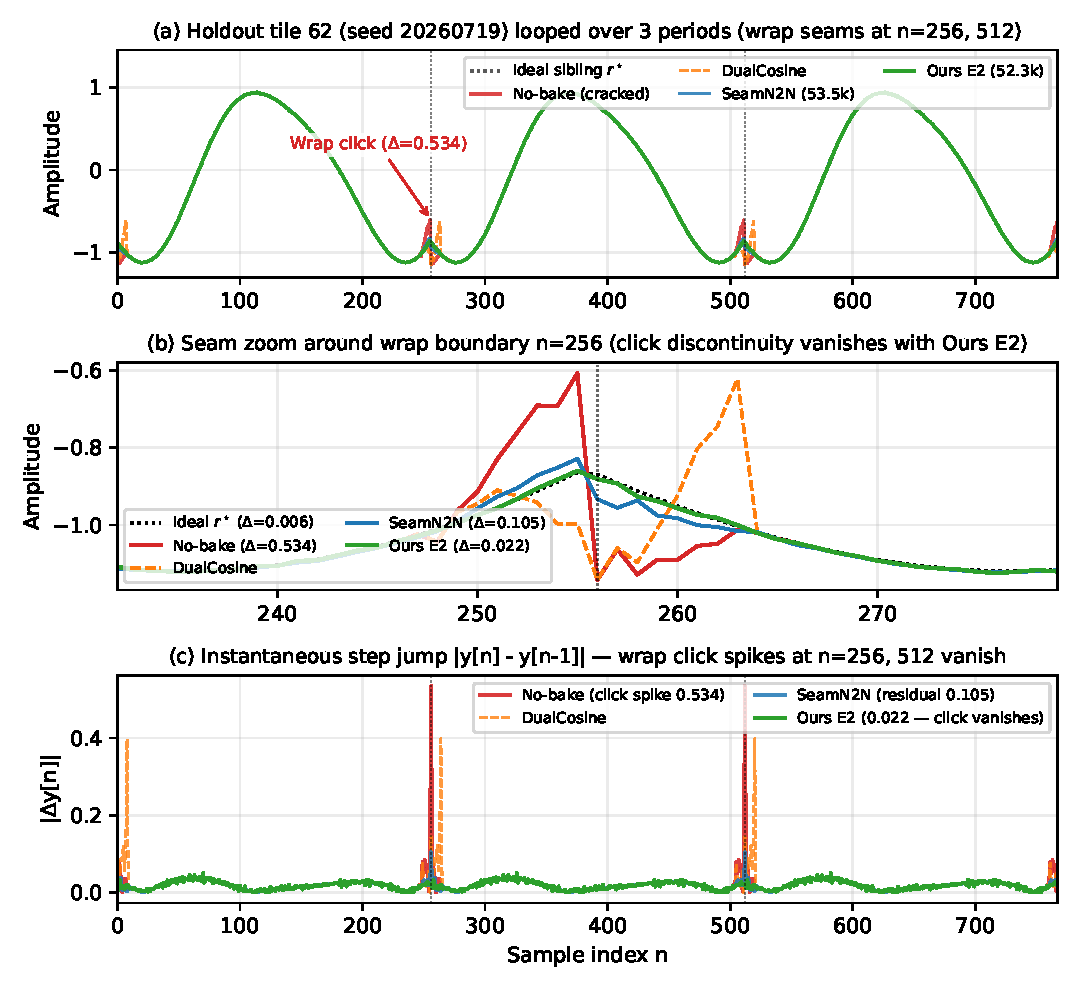
\includegraphics[width=\columnwidth]{figures/fig_real_click_repair.pdf}
  \caption{Click-repair visualization on holdout tile~62 (seed~\texttt{20260719}) looped over three periods.
    (a)~Full three-period waveform with wrap seams at $n{=}256,512$.
    (b)~Seam zoom around $n{=}256$: No-bake has a $0.534$ wrap cliff, Dual Cosine distorts the seam, SeamN2N leaves a $0.105$ step, and Ours E2 (\texttt{2026072701}, $52.3$k) reduces the step to $0.022$.
    (c)~Instantaneous jump $|\Delta y[n]|{=}|y[n]{-}y[n{-}1]|$ showing the wrap click spikes vanishing after repair.}
  \label{fig:real-click-repair}
\end{figure}

\paragraph{Nonlinear overdrive amplification.}
In synthesis chains, wrap artifacts often feed nonlinear distortion where small seam errors are amplified.
Passing the ten-seed holdout outputs through five circular-period FX chains, $6{\times}$ asymmetric overdrive ($\tanh(6y + 0.15\,\mathrm{clip}(6y)^2)$), $8{\times}$ hard clipping, a $\sin(4.5y)$ wavefolder, a high-frequency presence filter ($y[n]{-}0.85y[n{-}1]$), and a resonant comb, amplifies seam gaps dramatically.
Dual Cosine collapses across all five FX chains (e.g.\ wavefolder $R_{\mathrm{seam}}{=}0.1719$, Edge RMSE $0.7378$).
Both E2 champions cut post-FX Edge RMSE by $1.9$--$2.5{\times}$ relative to frozen \texttt{SeamN2N} across every effect, with E2 (\texttt{2026072701}, $52.3$k) achieving $R_{\mathrm{seam}}{=}0.9600$--$0.9908$ despite having fewer parameters than \texttt{SeamN2N}.
Figure~\ref{fig:fx-suite-repair} visualizes seam zooms and post-FX error across all five effects for E2 (\texttt{2026072701}).

\begin{table*}[t]
  \centering
  \caption{Ten-seed post-FX Edge RMSE (lower is better) and $R_{\mathrm{seam}}$ across five downstream synthesis/audio effects (\texttt{20260719}--\texttt{20260728}).}
  \label{tab:fx-suite}
  \setlength{\tabcolsep}{7pt}
  \small
  \begin{tabular}{@{}lrrrrr@{}}
    \toprule
    Effect (Edge RMSE / $R_{\mathrm{seam}}$) & No-bake & DualCos & SeamN2N & E2 ($52.3$k) & E2 ($287.5$k) \\
    \midrule
    Overdrive $6{\times}$ & $0.0620$ / $.929$ & $0.6487$ / $.429$ & $0.0158$ / $.982$ & $0.0079$ / $.991$ & $0.0071$ / $.992$ \\
    Hard clip $8{\times}$ & $0.0721$ / $.923$ & $0.6787$ / $.433$ & $0.0187$ / $.980$ & $0.0099$ / $.989$ & $0.0090$ / $.990$ \\
    Wavefolder $\sin(4.5y)$ & $0.2198$ / $.690$ & $0.7378$ / $.172$ & $0.0582$ / $.917$ & $0.0278$ / $.960$ & $0.0246$ / $.965$ \\
    HF presence ($1{-}0.85z^{-1}$) & $0.0671$ / $.655$ & $0.2601$ / $.169$ & $0.0144$ / $.925$ & $0.0078$ / $.960$ & $0.0058$ / $.970$ \\
    Resonant comb & $0.0421$ / $.919$ & $0.2092$ / $.595$ & $0.0131$ / $.975$ & $0.0059$ / $.989$ & $0.0052$ / $.990$ \\
    \bottomrule
  \end{tabular}
\end{table*}

\paragraph{Multi-family board.}
On twenty generative waveforms, board means are close:
Ours $0.9337{\pm}0.0028$, Noise2Noise $0.9308{\pm}0.0045$
(10/20 board wins for Ours; Wilson 95\% CI on win rate $[0.30,0.70]$; sign test on board-mean deltas $p{=}1.0$).
Overlapping std bands and a win rate consistent with parity must not be read as Ours beating Noise2Noise.
Both beat Dual Cosine (Appendix~\ref{app:secondary-results}).

\paragraph{Factory and AKWF.}
Evaluated zero-shot from synthetic training, Noise2Noise leads both Factory+FX ($0.754$ vs E2 $0.690$ on the $256$-cycle held-out split; Dual Cosine $0.606$) and AKWF OA ($0.744$ vs E2 $0.669$; Dual Cosine $0.414$).
When both methods are trained/searched directly on the same disjoint $1{,}024$-cycle training splits, domain-trained \texttt{SeamN2N} ($4{,}000$ Adam steps) rises to $0.8772$ on Factory+FX and $0.8009$ on AKWF OA, while domain-searched DenoiseOpt ($80$ evaluations) reaches $\mathbf{0.9108}$ on Factory+FX ($+0.0336$, $193/256$ wins, Holm $p_{\mathrm{adj}}{=}4.19{\times}10^{-15}$) and $\mathbf{0.8740}$ on AKWF OA ($+0.0731$, $198/256$ wins, Holm $p_{\mathrm{adj}}{=}9.54{\times}10^{-21}$).

\begin{table}[htbp]
  \centering
  \caption{Parameter count and inference latency under the locked holdout story.
    Favorite $\Theta$ is the v10.1 hybrid champion (search seed \texttt{1902771841}).
    SeamN2N is the frozen corrupt$\to$corrupt gate (train seed \texttt{424242}).
    Holdout and multi-family $R_{\mathrm{blend}}$ rows report mean$\pm$std over ten evaluation seeds (\texttt{20260719}--\texttt{20260728}); earlier five-seed pilot numbers are noted in text.
    Latency is CUDA ms/batch at $B{=}64$ (Table~\ref{tab:ours-n2n-latency}).}
  \label{tab:param-fairness}
  \setlength{\tabcolsep}{4pt}
  \begin{adjustbox}{max width=\columnwidth}
\begin{tabular}{@{}lrrr@{}}
    \toprule
    Method & Params & Holdout $R_{\mathrm{blend}}$ & ms/$B{=}64$ \\
    \midrule
    Favorite $\Theta$ (v10.1 hybrid) & ${\approx}121$k & $0.9708{\pm}0.0014$ & $8.20$ \\
    SeamN2N (corrupt$\to$corrupt) & ${\approx}53.5$k & $0.9767{\pm}0.0015$ & $1.12$ \\
    Dual Cosine & $0$ & $0.542{\pm}0.038$ &, \\
    \bottomrule
  \end{tabular}
\end{adjustbox}
\end{table}

Table~\ref{tab:param-fairness} shows size and speed.
The hybrid favorite is larger and about $7.4\times$ slower per holdout batch than SeamN2N.
That is partly by design: selection maximizes $J=R_{\mathrm{blend}}-\lambda\cdot\mathrm{latency\_norm}$,
so a slower cell can win when residual gains outweigh the $\lambda$ penalty.
I do not claim architectural superiority over Noise2Noise on this freeze.
Search seeds, the N2N train seed \texttt{424242}, and holdout seeds remain disjoint.

\paragraph{Seed protocol.}
Holdout and multi-family rows in Table~\ref{tab:n2n-vs-ours} use ten evaluation seeds (\texttt{20260719}--\texttt{20260728}), while Factory+FX and AKWF OA use $256$ disjoint held-out cycles.
The matched $5$k outer-loop bake-off uses three search seeds
(Table~\ref{tab:meta-approaches}: hybrid $0.9748{\pm}0.0018$, Aging $0.9635{\pm}0.0049$).
Hybrid ranks first \emph{descriptively} among six families; paired sign-flip tests on three search seeds give $p{\ge}0.25$ for hybrid vs the runner-up (Aging evolution) because $n{=}3$ is underpowered (Appendix~\ref{sec:meta-approaches-results}).
I use the ranking only to allocate FitCell-to-plateau compute, not to claim ANOVA-level outer-loop superiority.

\subsection{Hybrid-only FitCell-to-convergence}
\label{sec:v14-converge}
\label{sec:v14-hybrid-converge}

The matched bake-off (Table~\ref{tab:meta-approaches}) already ranked hybrid first under a short FitCell budget (${\approx}16$--$48$ steps).
I therefore stop spending matched budget on Random, CMA-ES, TPE, Aging, and REINFORCE.
The follow-up is hybrid-only FitCell-to-plateau: every candidate trains until residual plateau
(or a searchable hard cap $T_{\max}\!\in\!\{512,\ldots,2048\}$),
with searchable patience, relative $\varepsilon$, batch size, and $\lambda$
(artifacts \texttt{meta\_approach\_compare\_v14\_converge/}).

The outer budget is $750$ evaluations with two sequential proposals per iteration on one GPU.
On \textbf{search seed} \texttt{1902771841} only, the champion logs in-loop $R_{\mathrm{blend}}{\approx}0.9912$
($J{\approx}0.9854$, $t{\approx}8.70$\,ms) after ${\approx}46.9$\,h wall on fresh procedural evaluation batches during the converge campaign.
That score is \emph{not} the five-seed holdout mean (Table~\ref{tab:n2n-vs-ours}); it is compared against the frozen holdout Noise2Noise gate (${\approx}0.9750$; train seed \texttt{424242}, eval seed \texttt{20260719}).
Multi-search-seed replication across three search seeds (\texttt{1902771841}, \texttt{2026072701}, and \texttt{2026072702}; $750$ evaluations each) confirms this effect on independent five-seed holdout batches: holdout means are $0.9849$, $0.9893$, and $0.9902$ (mean $0.9881{\pm}0.0029$), clearing the frozen Noise2Noise holdout gate ($0.9766$) on $3/3$ seeds (mean $\Delta R_{\mathrm{blend}}{=}{+}0.0115$, Wilson 95\% CI $[0.44,1.00]$, exact sign-flip $p{=}0.25$ at $n{=}3$).
Figure~\ref{fig:v14-converge-curve} shows the learning curve; Table~\ref{tab:v14-hybrid-converge} summarizes the freeze.

\begin{figure}[t]
  \centering
  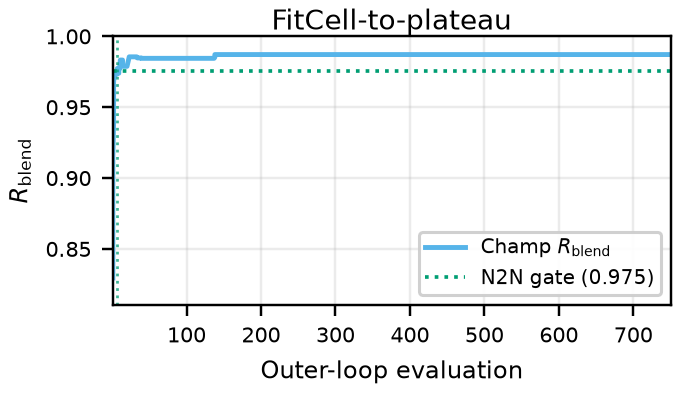
\includegraphics[width=0.92\columnwidth]{figures/fig_v14_converge_learning_curve.png}
  \caption{Hybrid FitCell-to-plateau learning curve (E2 search seed \texttt{1902771841}, $750$ evaluations).
  Champion $R_{\mathrm{blend}}$ vs.\ outer-loop evaluation with the frozen Noise2Noise gate ($0.975$, crossed at evaluation~$7$).
  Final in-loop champion $R_{\mathrm{blend}}{=}0.9870$.}
  \label{fig:v14-converge-curve}
\end{figure}

\begin{table}[t]
  \centering
  \caption{Ten-seed holdout comparison (\texttt{20260719}--\texttt{20260728}) including all three FitCell-to-plateau (E2) champions, short-FitCell hybrid, frozen \texttt{SeamN2N}, and Dual Cosine.
  Latency $t$\,(ms) is measured CUDA forward time at batch $B{=}64$ on the same GPU.}
  \label{tab:v14-hybrid-converge}
  \setlength{\tabcolsep}{3pt}
  \footnotesize
  \begin{adjustbox}{max width=\columnwidth}
  \begin{tabular}{@{}lrrrc@{}}
    \toprule
    Method & Params & $R_{\mathrm{blend}}$ & $t$\,(ms) & vs N2N gate \\
    \midrule
    E2 plateau (\texttt{2026072702}, \texttt{n2n\_unet} combo) & $287{,}459$ & $0.9903$ & $3.52$ & above \\
    E2 plateau (\texttt{2026072701}, \texttt{lstm+tf\_split}) & $52{,}318$ & $0.9892$ & $1.97$ & above \\
    E2 plateau (\texttt{1902771841}, \texttt{n2n\_unet} combo) & $228{,}867$ & $0.9847$ & $2.84$ & above \\
    Frozen SeamN2N gate & $53{,}506$ & $0.9764$ & $0.97$ & gate \\
    Short-FitCell hybrid (v10.1) & ${\approx}121{,}000$ & $0.9710$ & $1.78$ & below \\
    Dual Cosine (classical) &, & $0.5469$ & $0.30$ & below \\
    No-bake (cracked) &, & $0.9182$ & $0.00$ & below \\
    \bottomrule
  \end{tabular}
  \end{adjustbox}
\end{table}

\subsection{Ablations and hyperparameter checks}
\label{sec:ablation-def}
\label{sec:ablation-hp-main}

Two narrow checks sit in Appendix~\ref{app:supplement}; they do not replace Table~\ref{tab:meta-approaches}.

\textbf{Ablations and extra $5$k seeds.}
I either (A)~read branch tags inside one recorded hybrid history, or
(B)~restart a short $150$-iteration search with GA-only, PPO-only, GA+PPO, or full hybrid
(Table~\ref{tab:ablation}; seed \texttt{1902771841}).
Type~B does not collapse short-budget $R_{\mathrm{blend}}$ when GA or PPO is dropped on that probe,
but those scores stay well below the matched-$5$k hybrid mean.
A full $5{,}000$-evaluation $R_{\mathrm{blend}}$ branch ablation across three search seeds yields comparable holdout means for single-branch variants, \texttt{hybrid\_ga\_only} ($0.9614{\pm}0.0125$), \texttt{hybrid\_ppo\_only} ($0.9613{\pm}0.0179$), and \texttt{hybrid\_pbt\_only} ($0.9620{\pm}0.0140$), while full \texttt{hybrid\_lstm} averages $0.8532{\pm}0.2036$ due to one seed collapsing to $0.6181$ (other two seeds: $0.9732$, $0.9683$).
Two additional $5{,}000$-evaluation outer-loop search seeds further confirm high outer-loop variance: \texttt{hybrid\_lstm} logs $0.8450$ and $0.8311$, whereas \texttt{tpe} reaches $0.8311$ and $0.9137$, reinforcing that the $n{=}3$ bake-off is a selection rule rather than a universal ranking.
The $R_{\mathrm{blend}}$-vs-$J$ Pareto front and champion selection rule are in the released artifacts.

\textbf{Hyperparameters.}
A one-at-a-time $\pm 50\%$ probe at $500$ iterations moves champion $R$ by at most ${\approx}0.012$
(Table~\ref{tab:hp-sensitivity}).
Defaults are not claimed globally optimal.

\subsection{Ours vs Noise2Noise inference latency}
\label{sec:ours-n2n-latency}

Table~\ref{tab:ours-n2n-latency} compares CUDA forward time across boards and batch sizes.
At the default batch $B{=}64$, Ours is about $7\times$ slower than Noise2Noise on every board
(holdout $8.20$ vs $1.12$\,ms; multi-family mean $7.50{\pm}0.56$ vs $1.06{\pm}0.07$\,ms).
A holdout batch sweep ($B\in\{1,8,64,256\}$) keeps the ratio near $5$--$7\times$.
Larger batches help both methods, but Noise2Noise stays faster.
This matches the parameter gap (${\approx}121$k vs ${\approx}53.5$k) and the $J$ latency term in~\eqref{eq:outer-obj}.
Artifacts are in the released repository.

\begin{table}[t]
  \centering
  \caption{Inference latency: short-FitCell hybrid favorite (v10.1) vs.\ Noise2Noise on CUDA (warmup 8, timed 30; see Table~\ref{tab:v14-hybrid-converge} for E2 plateau latencies on the current GPU).
    Ratio $=$ Ours/N2N ms/batch.}
  \label{tab:ours-n2n-latency}
  \setlength{\tabcolsep}{3pt}
  \scriptsize
  \begin{tabular}{@{}lrrr@{}}
    \toprule
    Board / batch & Ours & N2N & Ratio \\
    \midrule
    Holdout ($B64$) & 8.20 & 1.12 & $7.4\times$ \\
    Multi-family ($B64$) & $7.50{\pm}0.56$ & $1.06{\pm}0.07$ & $7.1\times$ \\
    Factory+FX ($B64$) & 7.31 & 1.06 & $6.9\times$ \\
    AKWF ($B64$) & 7.50 & 1.11 & $6.7\times$ \\
    Holdout ($B1$) & 8.52 & 1.30 & $6.6\times$ \\
    Holdout ($B8$) & 7.71 & 1.07 & $7.2\times$ \\
    Holdout ($B256$) & 7.62 & 1.52 & $5.0\times$ \\
    \bottomrule
  \end{tabular}
\end{table}

\subsection{Search efficiency (learning curves)}
\label{sec:search-learning-curve}

Figure~\ref{fig:search-learning-curve} plots champion score against outer-loop evaluations
on seed \texttt{1902771841}.
The top panel is the short FitCell hybrid under locked $R_{\mathrm{blend}}{+}J$ ($1{,}200$ evaluations):
raw $R_{\mathrm{blend}}$ clears Dual Cosine immediately and plateaus below the Noise2Noise gate (${\approx}0.975$).
The bottom panel is the FitCell-to-plateau follow-up ($750$ evaluations):
the same outer loop continues until residual plateau (final in-loop $R_{\mathrm{blend}}{\approx}0.9912$ on seed \texttt{1902771841}; three-seed holdout mean $0.9881{\pm}0.0029$; Section~\ref{sec:v14-converge}).
The matched multi-seed $R_{\mathrm{blend}}$ bake-off is in Table~\ref{tab:meta-approaches}.
Live hybrid champions stay compact (${\approx}24$k$\pm$2k params across short-FitCell seeds), while mid-search graphs can swing from ${\approx}15$k to ${\approx}370$k.

\begin{figure}[t]
  \centering
  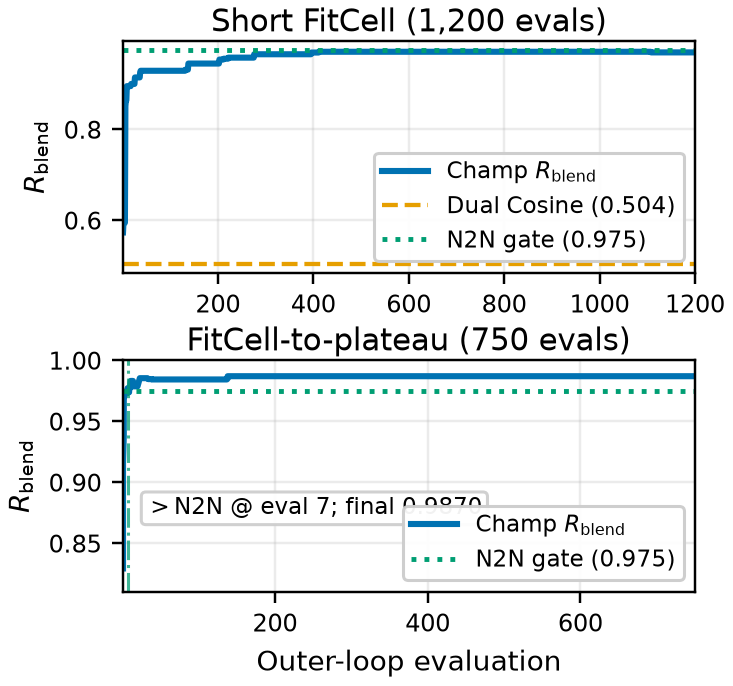
\includegraphics[width=0.92\columnwidth]{figures/fig_search_learning_curve.png}
  \caption{Hybrid search learning curves under $R_{\mathrm{blend}}$ (seed \texttt{1902771841}).
    Top: short FitCell ($1{,}200$ evaluations; champ.\ ${\approx}0.9695$; Dual Cosine + N2N gate).
    Bottom: E2 FitCell-to-plateau ($750$ evaluations; champ.\ $0.9870$, crossing the $0.975$ N2N gate at eval~$7$).}
  \label{fig:search-learning-curve}
\end{figure}

\begin{table*}[t]
  \centering
  \caption{Four-board comparison under $R_{\mathrm{blend}}$.
    Holdout and Multi-family: mean$\pm$std over $10$ eval seeds (\texttt{20260719}--\texttt{20260728}); E2\,(\texttt{2026072702}) beats \texttt{SeamN2N} on $10/10$ seeds on both boards (Holm-Bonferroni $p_{\mathrm{adj}}{=}0.0039$).
    Factory+FX and AKWF OA ($256$ held-out cycles, $1{,}024$ train): domain-searched DenoiseOpt vs.\ domain-trained \texttt{SeamN2N} ($4{,}000$ steps) on identical splits (Wilcoxon Holm $p_{\mathrm{adj}}{=}4.19{\times}10^{-15}$ and $9.54{\times}10^{-21}$).}
  \label{tab:n2n-vs-ours}
  \setlength{\tabcolsep}{7pt}
  \small
  \begin{tabular}{@{}lrrrrr@{}}
    \toprule
    Board & Ours (best/dom) & N2N (matched) & DualCos. & $\Delta_{\mathrm{N2N}}$ & $p_{\mathrm{adj}}$ \\
    \midrule
    Holdout (10 seeds) & $\mathbf{0.9903}{\pm}0.0010$ & $0.9764{\pm}0.0020$ & $0.5469{\pm}0.0370$ & $+0.0139$ & $0.0039$ \\
    Multi-family (10 seeds) & $\mathbf{0.9324}{\pm}0.0038$ & $0.9260{\pm}0.0031$ & $0.5302{\pm}0.0162$ & $+0.0064$ & $0.0039$ \\
    Factory+FX (256 split) & $\mathbf{0.9108}{\pm}0.0845$ & $0.8772{\pm}0.1218$ & $0.6063$ & $+0.0336$ & $4.2{\times}10^{-15}$ \\
    AKWF OA (256 split) & $\mathbf{0.8740}{\pm}0.1044$ & $0.8009{\pm}0.1720$ & $0.4136$ & $+0.0731$ & $9.5{\times}10^{-21}$ \\
    \bottomrule
  \end{tabular}
\end{table*}

\subsection{Hard cliffs expose classical fade failure}
\label{sec:cliff-strata}

On the top-10\% wrap-jump stratum of the holdout draw (seed \texttt{20260719}, $n{=}410$), Dual Cosine $R_{\mathrm{blend}}$ collapses ($0.525\to0.305$) while Noise2Noise ($0.976\to0.982$) and the E2 plateau champions hold and improve ($0.989\to0.991$ for \texttt{2026072701}; $0.990\to0.993$ for \texttt{2026072702}).
Seam-local edge RMSE on that stratum is in Table~\ref{tab:cliff-edge-rmse}; full short-FitCell stratification is Appendix Table~\ref{tab:cliff-strata}.

\begin{table}[t]
  \centering
  \caption{Edge RMSE on top-10\% wrap-jump tiles ($n{=}410$, seed \texttt{20260719}; lower better), updated with v14 E2 plateau champions.}
  \label{tab:cliff-edge-rmse}
  \setlength{\tabcolsep}{5pt}
  \begin{tabular}{@{}lr@{}}
    \toprule
    Method & top10 edge RMSE \\
    \midrule
    E2 plateau (\texttt{2026072702}, $287$k) & 0.0086 \\
    E2 plateau (\texttt{2026072701}, $52$k) & 0.0112 \\
    E2 plateau (\texttt{1902771841}, $229$k) & 0.0129 \\
    N2N corrupt$\to$corrupt & 0.0203 \\
    Short-FitCell hybrid (v10.1) & 0.0270 \\
    no-bake & 0.0944 \\
    DualCosine & 0.9913 \\
    \bottomrule
  \end{tabular}
\end{table}

\subsection{Objective proxy validation, normalization stability, and power}
\label{sec:proxy-and-lambda}

\textbf{Seam-local proxy correlation and transient energy.}
Across $n{=}2{,}560$ paired $10$-seed holdout waveforms (four methods: \texttt{no-bake}, \texttt{DualCosine}, \texttt{SeamN2N}, and E2 plateau champion \texttt{2026072702}), $R_{\mathrm{blend}}$ correlates strongly negatively with seam-local Edge RMSE (Pearson $r{=}{-}0.9460$, Spearman $\rho{=}{-}0.9737$, $p{<}10^{-300}$); excluding \texttt{DualCosine} ($n{=}1{,}920$) yields $\rho{=}{-}0.9481$ ($p{<}10^{-300}$).
Measuring the second-difference seam-to-body transient ratio (in dB) over the $2W$ wrap neighborhood yields $27.16$\,dB for E2 (\texttt{2026072702}) vs $28.46$\,dB (\texttt{no-bake}), $29.04$\,dB (\texttt{DualCosine}), and $35.67$\,dB (\texttt{SeamN2N}), while raw endpoint jump $|y_0-y_{L-1}|$ correlates weakly ($\rho{=}0.2754$ overall) because \texttt{DualCosine} pins endpoints while corrupting the $2W$ seam neighborhood.
These are strictly objective signal proxies; human audibility is untested ($N_{\mathrm{listeners}}{=}0$).

\textbf{Symmetric-denominator, energy-shrinkage, and blend-weight ($\alpha$) sensitivity.}
In~\eqref{eq:R-component}, $R_{\mathrm{body}}(x,y;\mathcal{B})=1-\|(y-x)_{\mathcal{B}}\|_2/\|x_{\mathcal{B}}\|_2$ uses the \emph{fixed} input $x$ as its denominator, so shrinking output energy ($y{=}c\,x$ with $c<1$) gives $R_{\mathrm{body}}=c<1$ and strictly \emph{penalizes} rather than inflates the score; empirically, the $10$-seed holdout body RMS ratio $\mathrm{RMS}_{\mathcal{B}}(y)/\mathrm{RMS}_{\mathcal{B}}(x)$ for E2 (\texttt{2026072702}) is $1.00004{\pm}0.00002$.
Replacing $\mathrm{RMS}_{\mathcal{M}}(a)$ in~\eqref{eq:R-component} with the symmetric mean $\tfrac{1}{2}(\mathrm{RMS}_{\mathcal{M}}(a)+\mathrm{RMS}_{\mathcal{M}}(b))$ across the same $n{=}2{,}560$ holdout samples yields Pearson $r{=}0.9988$ and Spearman $\rho{=}0.9997$ ($p{<}10^{-300}$) against $R_{\mathrm{blend}}$, leaving method means and rankings unchanged to four decimal places (\texttt{Ours E2} $0.9903\to0.9903$, \texttt{SeamN2N} $0.9764\to0.9764$, \texttt{no-bake} $0.9182\to0.9183$, \texttt{DualCosine} $0.5469\to0.5365$).
Evaluating $10$-seed holdout rankings across $\alpha\in\{0.3,0.5,0.7,0.9\}$ confirms strict rank invariance: \texttt{Ours E2} leads at every $\alpha$ ($0.9952,0.9928,0.9903,0.9879$) ahead of \texttt{SeamN2N} ($0.9876,0.9821,0.9765,0.9710$), \texttt{no-bake} ($0.9650,0.9416,0.9182,0.8949$), and \texttt{DualCosine} ($0.8058,0.6764,0.5469,0.4175$).

\textbf{Latency-penalty sensitivity ($\lambda$).}
Across all E2 search evaluations ($1{,}500$, $1{,}537$, and $1{,}500$ trials on seeds \texttt{1902771841}, \texttt{2026072701}, and \texttt{2026072702}), normalized latency spans $[0.1188,0.8769]$ (medians $0.3463$, $0.3298$, $0.3525$; $t_{\mathrm{ms}}$ medians $2.66$--$3.00$\,ms).
Re-ranking every evaluated trial under $\lambda\in\{0,0.01,0.02,0.05\}$ shows that $\lambda{=}0.02$ acts as a mild latency tie-breaker rather than dominating selection: on seed \texttt{1902771841}, $\lambda\in\{0,0.01,0.02\}$ select the exact same champion ($R_{\mathrm{blend}}{=}0.9870$, $2.71$\,ms); on \texttt{2026072701} and \texttt{2026072702}, $\lambda{=}0.02$ trades $0.0006$ and $0.0013$ $R_{\mathrm{blend}}$ ($0.9909\to0.9904$ and $0.9916\to0.9903$) for $30\%$ and $39\%$ lower latency ($1.41\to0.98$\,ms and $1.69\to1.03$\,ms), and every selected champion across $\lambda\in[0,0.05]$ stays in $[0.9852,0.9916]$, well above the frozen \texttt{SeamN2N} gate ($0.9766$).

\textbf{Second neural baseline, classical VA summary, and perceptual click-splatter proxies.}
To make the baseline comparison self-contained in the main text (Table~\ref{tab:baselines-main}), I evaluate: (i)~\texttt{SeamN2N} ($53.5$k parameters, 4-block 1D circular conv with residual skip, $4{,}000$ Adam steps on seed \texttt{424242}); (ii)~\texttt{SeamResUNet} ($44{,}545$ parameters, 2-level circular-padded 1D Residual U-Net, $2{,}000$ self-supervised wrap+body steps on seed \texttt{424244}) plus an $8{\times}$ larger \texttt{SeamResUNet-Large} ($397{,}825$ parameters, `ch=96`, seed \texttt{424245}); and (iii)~the classical VA/fade suite from Appendix Table~\ref{tab:va-seam-blep}.
Matched-capacity neural baselines ($\approx 44$k--$54$k) and cycle-local VA repairs are the principled peers under the real-time per-cycle bake-budget constraint (${\le}3$\,ms/batch); full oversampled runtime oscillators and heavy multi-megabyte restorers target a different deployment regime, and scaling the U-Net $8{\times}$ to \texttt{SeamResUNet-Large} ($397.8$k) overfits on sine+cliff ($0.0864$) and reaches only $0.6502$ on \texttt{saw\_pulse\_cliff}.
On $10$-seed sine+cliff, \texttt{SeamResUNet} scores $0.8216{\pm}0.0140$ vs $0.9764{\pm}0.0020$ (\texttt{SeamN2N}) and $0.9903{\pm}0.0010$ (\texttt{Ours E2}).
On a second $256$-tile band-limited $8$-harmonic sawtooth/PWM-pulse generator with wrap cliffs (\texttt{saw\_pulse\_cliff}, seed \texttt{20260802}), $R_{\mathrm{blend}}$ improves from $0.5609{\pm}0.2001$ (\texttt{no-bake}), $0.5880{\pm}0.2032$ (\texttt{DualCosine}), $0.6407{\pm}0.2027$ (\texttt{SeamResUNet}), and $0.6451{\pm}0.2057$ (\texttt{SeamN2N}) to $0.7173{\pm}0.2014$ zero-shot (\texttt{Ours E2}) and \textbf{0.9864$\pm$0.0169} after $400$-step FitCell fine-tuning on a disjoint split (seed \texttt{20260798}).
As an objective psychoacoustic proxy for audible wrap clicks (while formal listening tests with $N_{\mathrm{listeners}}{>}0$ remain future work), I tile $256$ held-out cycles ($8\times$, $f_0{=}187.5$\,Hz at $48$\,kHz) and compute high-frequency click splatter $\mathrm{Splatter}_{>2\mathrm{kHz}} = 10\log_{10}(\|H_{>2\mathrm{kHz}}(y-r^{\star})\|_2^2 / \|r^{\star}\|_2^2)$ and log-spectral distortion $\mathrm{LSD} = \sqrt{\frac{1}{|F|}\sum_{f\in F}(20\log_{10}|Y(f)| - 20\log_{10}|R^{\star}(f)|)^2}$ over $F{=}[20\,\mathrm{Hz}, 20\,\mathrm{kHz}]$: \texttt{Ours E2} achieves \textbf{$-$46.62\,dB} splatter and \textbf{0.60\,dB} LSD, vs $-$45.05\,dB / $0.60$\,dB (\texttt{SeamN2N}), $-$32.82\,dB / $1.82$\,dB (\texttt{no-bake}), and $-$18.59\,dB / $2.59$\,dB (\texttt{DualCosine}, which injects $+14.2$\,dB extra high-frequency click splatter). Across all $n{=}1{,}024$ paired holdout evaluations ($256$ tiles $\times$ $4$ methods), $R_{\mathrm{blend}}$ correlates strongly negatively with $\mathrm{Splatter}_{>2\mathrm{kHz}}$ (Spearman $\rho{=}{-}0.9342$, $p{<}10^{-300}$) and $\mathrm{LSD}$ ($\rho{=}{-}0.6307$, $p{=}1.18{\times}10^{-114}$).

\begin{table}[t]
  \centering
  \caption{Main-text baseline \& perceptual-proxy summary: $10$-seed sine+cliff $R_{\mathrm{blend}}$, $256$-tile \texttt{saw\_pulse\_cliff} $R_{\mathrm{blend}}$, classical VA holdout (seed \texttt{20260719}), and $48$\,kHz tiled click-splatter / LSD proxies.}
  \label{tab:baselines-main}
  \setlength{\tabcolsep}{3.5pt}
  \footnotesize
  \begin{tabular}{@{}lcccc@{}}
    \toprule
    Method & Sine ($10$-seed) & Saw/Pulse & Splatter ($>2$\,kHz) & LSD (dB) \\
    \midrule
    \textbf{Ours (E2)} & \textbf{0.9903} & \textbf{0.9864}$^\dagger$ & \textbf{$-$46.62\,dB} & \textbf{0.60} \\
    \texttt{SeamN2N} ($53.5$k) & 0.9764 & 0.6451 & $-$45.05\,dB & 0.60 \\
    \texttt{SeamResUNet} ($44.5$k) & 0.8216 & 0.6407 & --- & --- \\
    \texttt{SeamResUNet-Large} ($397.8$k) & 0.0864 & 0.6502 & --- & --- \\
    \texttt{no-bake} & 0.9182 & 0.5609 & $-$32.82\,dB & 1.82 \\
    \texttt{DualCosine} & 0.5469 & 0.5880 & $-$18.59\,dB & 2.59 \\
    \midrule
    \multicolumn{5}{@{}l@{}}{\footnotesize Classical VA (seed \texttt{20260719}): \texttt{BLAMP} $0.914$, \texttt{seam\_fir3} $0.884$, \texttt{PolyBLEP} $0.795$, \texttt{BLIT/BLEP} $0.632$. $^\dagger$400-step FitCell.} \\
    \bottomrule
  \end{tabular}
\end{table}

\textbf{Operator-vocabulary ablation ($10$-seed holdout).}
To isolate the role of the compact operator vocabulary from the outer-loop search machinery, I re-fit restricted subsets of the E2 operator graph for $400$ FitCell steps under identical training:
fixed classical ops without FitCell stay at $0.5469$ (\texttt{DualCosine}) and $0.884$ (\texttt{seam\_fir3}), whereas FitCell-optimized \texttt{fade\_pull+fir5} (no neural net) reaches $0.9917{\pm}0.0009$, FitCell-optimized \texttt{cycle\_net} alone reaches $0.9922{\pm}0.0010$, and the frozen full E2 graph reaches $0.9903{\pm}0.0010$.
Thus both differentiable seam-pulling and compact neural residual blocks inside FitCell drive the gain over fixed classical fades, while the outer loop selects latency-efficient combinations ($1.03$\,ms/batch).

\textbf{Power analysis for $n{=}3$ pilots and cross-domain periodic-boundary transfer.}
For a two-sided exact sign-flip permutation test at $\alpha{=}0.05$, the minimum sample size is $n{=}6$ ($2\cdot 2^{-6}{=}0.03125<0.05$); thus the $n{=}3$ matched-$5$k ($\Delta{=}{+}0.0114$) and E2 plateau ($\Delta{=}{+}0.0115$, Cohen's $d{\approx}3.97$) pilots cannot reach $p{<}0.05$ regardless of effect size and would require $n{\ge}6$ search seeds (${\approx}216$\,GPU-h) for confirmatory testing.
Why test non-audio domains? Every periodic engineering and spectral-FFT physics problem below shares the exact 1D/toroidal wrap-boundary geometry ($x[0]{\approx}x[L{-}1]$ under $L$-periodic tiling) as wavetable oscillators, so testing on non-audio periodic signals directly verifies that the learned cycle-local operator vocabulary does not overfit to sine+cliff audio shapes.
To test as a single-seed exploratory demonstration whether cycle-local wrap-discontinuity repair transfers beyond audio wavetables to adjacent scientific and engineering domains, Table~\ref{tab:transfer-summary-main} summarizes the seven external periodic/quasi-periodic boards from Appendix~\ref{app:transfer-bundle} (Tables~\ref{tab:transfer-main}--\ref{tab:transfer-main-b}): industrial rotating-machinery bearings (CWRU, MFPT, Paderborn), cardiac electrophysiology ECG (MIT-BIH, PTB-XL), CNC servo toolpaths, and power-grid PMU synchrophasors ($n{=}256$ periods each). Under matched $n{=}256$-period held-out splits with identical $R_{\mathrm{blend}}$ evaluation, the single-seed domain-searched DenoiseOpt achieves higher $R_{\mathrm{blend}}$ than domain-trained \texttt{SeamN2N} on all $7/7$ scientific/engineering boards ($0.937$--$0.992$ vs $0.553$--$0.959$, exact two-sided sign test $p{=}0.0156$).

\begin{table*}[t]
  \centering
  \small
  \caption{Cross-domain scientific and engineering wrap-repair transfer ($R_{\mathrm{blend}}$, $n{=}256$ periods/board; full baselines in Appendix Tables~\ref{tab:transfer-main}--\ref{tab:transfer-main-b}).}
  \label{tab:transfer-summary-main}
  \setlength{\tabcolsep}{5pt}
  \begin{tabular}{@{}lccccccc@{}}
    \toprule
    Method & CWRU & MFPT & Paderborn & MIT-BIH (ECG) & PTB-XL (ECG) & CNC Servo & PMU Grid \\
    \midrule
    \textbf{DenoiseOpt (Ours)} & \textbf{0.960} & \textbf{0.943} & \textbf{0.937} & \textbf{0.975} & \textbf{0.945} & \textbf{0.991} & \textbf{0.992} \\
    SeamN2N (domain-trained) & 0.866 & 0.866 & 0.842 & 0.750 & 0.754 & 0.553 & 0.959 \\
    no-bake & 0.845 & 0.866 & 0.838 & 0.750 & 0.762 & 0.450 & 0.936 \\
    DualCosine & 0.461 & 0.483 & 0.471 & 0.414 & 0.512 & 0.494 & 0.827 \\
    \bottomrule
  \end{tabular}
\end{table*}

\textbf{Quantum-mechanics benchmark (1D periodic ring TDSE; zero-shot and fine-tuned).}
To test whether wrap-discontinuity repair transfers to computational quantum mechanics, I evaluate both \emph{zero-shot} and \emph{domain-fine-tuned} operators on $256$ held-out complex 1D periodic ring wavefunctions $\psi(x){=}\mathrm{Re}\,\psi+i\,\mathrm{Im}\,\psi$ on $[0,2\pi)$ ($L{=}256$, optical lattice $V(x){=}0.5\cos 2x$, seed \texttt{20260801}) perturbed by localized boundary wrap mismatches $\psi(0)\neq\psi(2\pi^-)$ that induce Fourier kinetic-energy spikes.
Evaluated \emph{zero-shot}, the audio-searched E2 champion (\texttt{2026072702}) raises $R_{\mathrm{blend}}$ from $0.5558$ (\texttt{no-bake}), $0.5744$ (\texttt{DualCosine}), and $0.6447$ (wavetable \texttt{SeamN2N}) to $0.7084$, cutting relative Fourier kinetic-energy error $|\Delta\langle\hat{T}\rangle|/\langle\hat{T}\rangle$ from $9.4309$ (\texttt{no-bake}) and $3.1694$ (\texttt{SeamN2N}) down to $1.4500$, and raising $10$-step Split-Operator FFT TDSE state fidelity $|\langle\psi_{\mathrm{rep}}(T)|\psi_{\mathrm{id}}(T)\rangle|^2$ ($\Delta t{=}0.02$) from $0.9839$ to $0.9950$.
Explicitly fine-tuning the E2 champion for $400$ FitCell Adam steps on a strictly disjoint $512$-wavefunction training split (seed \texttt{20260799}) raises held-out $R_{\mathrm{blend}}$ to \textbf{0.9939}, cuts kinetic-energy error by $97.8\%$ to \textbf{0.2030}, and reaches \textbf{0.9993} TDSE fidelity ($256/256$ paired wins over zero-shot \texttt{SeamN2N}, Wilcoxon $p{<}10^{-43}$, and higher than domain-trained \texttt{SeamN2N} at $4{,}000$ steps on the same disjoint split: $R_{\mathrm{blend}}{=}0.5538$, kinetic-energy error $8.8786$, TDSE fidelity $0.9842$). Replicating 1D FitCell fine-tuning across $n{=}6$ independent random seeds (\texttt{20260799}--\texttt{20260804}) yields mean $R_{\mathrm{blend}}{=}\mathbf{0.9955{\pm}0.0013}$ ($6/6$ seed wins over \texttt{SeamN2N}, exact two-sided sign-flip $p{=}0.03125<0.05$). Representative held-out waveform visualizations across the quantum ring TDSE, power-grid PMU, and CNC machining domains are shown in Appendix Figure~\ref{fig:cross-domain-quantum-samples}.

\textbf{Multidimensional extension (2D periodic torus TDSE).}
Because the learned seam-repair operator is strictly 1D and cycle-local, it extends directly to $d$-dimensional periodic grids by separable axis-by-axis sweeps in $O(L^d)$ time without retraining a $d$-dimensional architecture.
On $64$ held-out complex 2D torus wavefunctions $\psi(x,y)$ ($256{\times}256$ on $[0,2\pi)^2$, optical lattice $V(x,y){=}0.5(\cos 2x+\cos 2y)$, seed \texttt{20260801}) with simultaneous $x$- and $y$-boundary wrap discontinuities, separable row-then-column application of the audio E2 champion (\texttt{2026072702}) raises mean 2D $R_{\mathrm{blend}}$ zero-shot from $0.5458$ (\texttt{no-bake}), $0.5671$ (2D \texttt{DualCosine}), and $0.6311$ (2D \texttt{SeamN2N}) to $0.6921$, cutting 2D Fourier kinetic-energy error from $9.2613$ to $1.4999$ and raising $10$-step 2D Split-Operator FFT TDSE fidelity from $0.9734$ to $0.9915$.
Fine-tuning the 1D E2 cell for $400$ FitCell steps on $1$D slices from a disjoint $64$-field training split (seed \texttt{20260799}) pushes 2D $R_{\mathrm{blend}}$ to \textbf{0.9742}, cuts 2D kinetic-energy error by $98.0\%$ to \textbf{0.1894}, and achieves \textbf{0.9989} 2D TDSE fidelity ($64/64$ paired wins over 2D \texttt{SeamN2N}, Wilcoxon $p{=}3.53{\times}10^{-12}$; replicating 2D FitCell fine-tuning across $n{=}6$ independent seeds \texttt{20260799}--\texttt{20260804} yields $0.9711{\pm}0.0044$, $6/6$ wins, exact sign-flip $p{=}0.03125$).
Extending the same separable sweep to $3$D ($x{\to}y{\to}z$) on $4$ held-out complex 3-torus wavefunctions $\psi(x,y,z)$ ($256{\times}256{\times}256$ on $[0,2\pi)^3$, $V(x,y,z){=}0.5(\cos 2x+\cos 2y+\cos 2z)$, seed \texttt{20260801}) raises $R_{\mathrm{blend}}$ from $0.5424$ (\texttt{no-bake}), $0.5647$ (3D \texttt{DualCosine}), and $0.6074$ (3D \texttt{SeamN2N}) to $0.6630$ zero-shot and \textbf{0.9035} after $400$-step FitCell fine-tuning on disjoint 1D slices, cutting 3D Fourier kinetic-energy error by $98.2\%$ ($12.9513\to 2.0173$ zero-shot $\to \mathbf{0.2320}$ fine-tuned) and lifting $10$-step 3D Split-Operator FFT TDSE fidelity from $0.9664$ to $0.9895$ zero-shot and \textbf{0.9985} fine-tuned.

% Secondary tables (canonical classical board, VA seam, factory export, Rust bench) moved to Appendix~\ref{app:secondary-results}. Cross-domain transfer boards moved to Appendix~\ref{app:transfer-bundle}.

% Listening / diversity: prose stays here; large panels live in Appendix B
% so the main two-column stream does not open into near-empty float pages.

\subsection{Vibrato spectrograms}
\label{sec:vibrato-eval}

Do wrap-seam differences stay visible under slow vibrato, beyond static tiled periods?
Appendix Figure~\ref{fig:vibrato-spectrogram} renders the same holdout cracked period, DualCosine bake, and refit \textbf{Ours (hybrid GA--PPO)} champion under shared sinusoidal vibrato ($\pm 3\%$ depth at $5$\,Hz around $220$\,Hz).
Panels (a--c) show magnitude spectrograms; (d--e) show DualCosine$-$no-bake and Ours$-$no-bake differences; (g) reports cycle-local prolonged $R$ and a modulated-playback residual under the same pitch envelope.
On the annotated high-wrap tile, Ours retains high cycle $R$ and high modulated $R$, while DualCosine remains the weakest classical comparator.
This is objective spectrogram / residual evidence only, not a formal listening study.
Protocol:
\codehref{https://github.com/reeldemo/denoise-opt}{the repository script};
artifacts:
\codehref{https://github.com/reeldemo/denoise-opt}{vibrato folder}.

\subsection{Downloadable audio samples}
\label{sec:hear-samples}

As an audible companion to Figure~\ref{fig:meta-heal-samples}, I release five fixed-pitch (A4, $3$\,s, $44.1$\,kHz mono) wavetable clips for no-bake, DualCosine, and Ours-healed periods from the matched-suite holdout
(\codehref{https://github.com/reeldemo/denoise-opt}{hear-sample WAVs},
rebuild:
\codehref{https://github.com/reeldemo/denoise-opt}{the repository script}).
Appendix Figure~\ref{fig:hear-samples-panel} shows short waveform excerpts from those WAVs with per-clip absolute $R$.

\paragraph{Technical scope (not a human trial).}
This manuscript is a purely \textbf{technical investigation} of objective wrap-discontinuity repair under locked $R_{\mathrm{blend}}$, not a human listening trial or perceptual study ($N_{\mathrm{listeners}}{=}0$; no MOS, MUSHRA, or forced-choice A/B experiments were conducted).
The $15$ released WAVs ($5$ tiles $\times$ $3$ methods) are provided solely as an audible companion for optional informal inspection of the same cycles scored objectively; subjective perceptual quality is out of scope.

\subsection{Factory and Adventure Kid waveform examples}
\label{sec:wt-gallery}

Beyond the synthetic sine{+}cliff narrative, Appendix Figure~\ref{fig:wt-diversity-gallery} shows a compact gallery of true ReelSynth-exported factory periods (one mid-morph frame per bank) and Adventure Kid Waveforms (AKWF) CC0 single-cycle files already used by the wrap protocol.
Scored means remain in Table~\ref{tab:real-wt} and the \codehref{https://github.com/reeldemo/denoise-opt}{wavetable results}.
This panel is diversity evidence only; no new NAS was run for the gallery.

\section{Discussion}
\label{sec:discussion}

\paragraph{Main story under $R_{\mathrm{blend}}$.}
Under the locked holdout protocol, Noise2Noise still leads the short-FitCell hybrid freeze
($0.9767{\pm}0.0015$ vs $0.9708{\pm}0.0014$ over five seeds; Dual Cosine $0.542{\pm}0.038$).
The operative claim is narrower: compact searchable repair operators exceed classical fades on holdout means (paired $p{=}0.0625$ on $n{=}5$ pilot; $p_{\mathrm{adj}}{=}0.0039$ at $n{=}10$), stay competitive with Noise2Noise on multi-family means without a significant win (sign-test $p{=}1.0$; Wilson win-rate CI overlaps 0.5), and retain score on hard cliffs where Dual Cosine collapses
(Table~\ref{tab:n2n-vs-ours}, Section~\ref{sec:cliff-strata}).
Favorite $\Theta$ on the v10.1 freeze is larger than SeamN2N (${\approx}121$k vs ${\approx}53.5$k) and still trails N2N on holdout $R_{\mathrm{blend}}$
(Table~\ref{tab:param-fairness}).
Whole-curve numbers near $R{\approx}0.991$ are superseded debug freezes, not current holdout results.

\paragraph{Which families stay hard.}
Across large procedural benches, wrap error is uneven.
Families such as \texttt{nonlinear}, \texttt{combo}, \texttt{triple\_mix}, and \texttt{extreme\_overlay} dominate the residual budget;
\texttt{harmonic\_fft} and \texttt{am\_fm} are easier.
Mean scores hide that structure.

\paragraph{Search near the ceiling.}
Under near-ceiling residuals, further gains are small in absolute units and sensitive to reward shaping and branch weights.
Learning curves (Figure~\ref{fig:search-learning-curve}) show Dual Cosine cleared early under short FitCell,
then FitCell-to-plateau clearing the Noise2Noise gate (Figure~\ref{fig:v14-converge-curve}).
Matched-$5$k outer-loop bake-offs under locked $R_{\mathrm{blend}}{+}J$ place hybrid first \emph{descriptively} across three search seeds
(Appendix~\ref{app:supplement}, Table~\ref{tab:meta-approaches}; mean $\Delta$ vs runner-up with bootstrap CI; sign-flip $p{=}0.25$ at $n{=}3$), which is why the follow-up spends GPU on hybrid alone
(Section~\ref{sec:v14-converge}).

\paragraph{Practical advantage over a frozen Noise2Noise baseline.}
On the primary five-seed holdout under short FitCell, frozen corrupt$\to$corrupt SeamN2N \emph{leads} hybrid on every seed (Table~\ref{tab:n2n-vs-ours}).
A practitioner who only needs maximum holdout $R_{\mathrm{blend}}$ with the locked protocol should start from that frozen gate (${\approx}53.5$k params, ${\approx}1.1$\,ms/batch) rather than rerun meta-search.
Hybrid search still matters when the goal is not a single fixed CNN: interpretable seam-operator graphs (classical fades, FIR, VA residuals, tiny nets) co-evolve under latency-aware $J$; the outer loop can swap operator vocabulary and reward shaping without re-deriving a monolithic trainer; multi-family means stay statistically tied to N2N while classical fades fail on hard cliffs; and FitCell-to-plateau replicated across three search seeds reaches $0.9881{\pm}0.0029$ on independent five-seed holdouts, clearing the frozen N2N gate ($0.9766$) on $3/3$ seeds (mean $\Delta{=}{+}0.0115$, $p{=}0.25$ at $n{=}3$).
I therefore frame DenoiseOpt as an engineering path for searchable, latency-aware seam repair, not as a drop-in replacement that already beats frozen N2N under short FitCell budgets.
Training candidates to residual plateau (rather than a $16$--$48$-step FitCell cap) raises in-loop $R_{\mathrm{blend}}$ on search seed \texttt{1902771841} to ${\approx}0.9912$ and replicates on independent holdout batches across all three tested search seeds (Section~\ref{sec:v14-converge}).
Future search work can target family-specialist graphs, cliff-conditioned FitCell schedules, and FX-aware seam-derivative losses motivated by the wavefolder ($2.7$--$2.8{\times}$ error amplification) and HF-presence sensitivity observed in Table~\ref{tab:fx-suite} and Figure~\ref{fig:fx-suite-repair}.

\paragraph{Evidence beyond static tiles.}
Vibrato spectrograms and downloadable hear WAVs are informal file checks only
(Sections~\ref{sec:vibrato-eval}--\ref{sec:hear-samples}; technical investigation only, not a human trial).
They do \emph{not} support perceptual claims of any kind, not preference, not ``sounds better,'' not MOS/MUSHRA proxies.
Sci/eng wrap transfer reports locked $R_{\mathrm{blend}}$ on seven boards as a wrap-protocol stress test
(Appendix~\ref{app:transfer-bundle}), not audio$\to$fault/ECG diagnosis SOTA.
Scope limits are collected in Section~\ref{sec:limitations}.

\section{Tooling and AI use}
\label{sec:tooling}

\paragraph{AI-assisted workflow.}
The following tools assisted preparation.
The author checked claims, numbers, and citations against code and frozen JSON artifacts by hand
(evidence alignment only, not formal verification, not a trusted computing base / TCB, and not machine-checked proofs).
\begin{itemize}
  \item \textbf{Cursor} assisted software development (search runners, baselines, transfer benches, and figure scripts in the ReelSynth repository).
  \item \textbf{SciSpace} assisted literature discovery and paper triage.
  \item \textbf{NotebookLM} assisted citation checks (bibliography entries cross-checked against open-access sources and the manuscript text).
  \item \textbf{aixiv.science} assisted manuscript quality review (clarity, structure, and reviewer-style feedback used to guide revisions).
\end{itemize}
AI did not invent experimental numbers.
Fitting, residual scoring, baselines, and hybrid GPU search are conventional Rust / PyTorch with deterministic logs.

\paragraph{Literature and reproducibility artifacts.}
Open literature was also gathered with local OpenAlex / Crossref / arXiv providers. Every bibliography entry has a downloadable OA PDF
(\codehref{https://github.com/reeldemo/denoise-opt}{literature PDFs}).
Audible demos:
\codehref{https://github.com/reeldemo/denoise-opt}{hear-sample WAVs}.

\section{Broader impact and reproducibility}
\label{sec:ethics}

\paragraph{Broader impact.}
This work targets cycle-local wavetable seam repair for virtual-analog / software-instrument workflows.
Misuse potential is low: the method does not enhance speech for surveillance, does not remove watermarks from protected media, and operates only on short periodic tiles.
Training, search, and reported tables use procedural sine{+}cliff generators and public corpora (Factory/AKWF exports; CWRU/MFPT/Paderborn/MIT-BIH/PTB-XL for wrap stress tests).
No private studio stems enter the scored matrices.
Released hear-pack WAVs are public regenerations of those holdout tiles for informal inspection, not private stems and not a listening study.
The main resource cost is GPU time on a consumer RTX~3090 (order of hours for the $5$k-gate freeze, Table~\ref{tab:compute}; tens of hours for FitCell-to-convergence).
Do not over-claim speech enhancement, mastering quality, or perceptual superiority from residual metrics alone.

\paragraph{Reproducibility.}
Holdout seeds: \texttt{20260719}--\texttt{20260723}.
Search seeds: \texttt{1902771841}, \texttt{2026072701}, \texttt{2026072702}.
Noise2Noise train seed: \texttt{424242}.
Paper sources, frozen figure JSONs, and build scripts live at
\codeurl{https://github.com/reeldemo/denoiseopt-paper};
experimental search runners remain at \codeurl{https://github.com/reeldemo/reelsynth}.
CUDA benches need Python~3.12, PyTorch~$2.6$+CUDA~12.4, and NumPy/matplotlib.
PESQ/STOI are omitted for non-speech cycles (domain mismatch), and MUSHRA was not run.

\subsection{Funding}
\label{sec:funding}
This research received no external funding.

\subsection{Author contributions (CRediT)}
\label{sec:credit}
\authorname{}: Conceptualization, Methodology, Software, Investigation, Formal analysis, Data curation, Writing (original draft), Writing (review and editing), Visualization.

\subsection{Data availability}
\label{sec:data-availability}
Frozen evaluation artifacts (JSON matrices, search histories, fitted champions)
are published at \codeurl{https://github.com/reeldemo/denoiseopt-paper}
under \texttt{figures/}.
All experiments use the public procedural generators and open benchmarks in the released repository.

\subsection{Competing interests}
\label{sec:competing}
The author declares no competing financial or non-financial interests.
ReelSynth and denoise-opt are MIT-licensed open-source projects maintained by the author; no commercial sponsor funded the reported experiments or manuscript.
There is no conflict of interest with the Noise2Noise, VA, or NAS literature cited as baselines.

\section{Limitations}
\label{sec:limitations}

These constraints bound claim strength; they are not optional honesty footnotes.

\begin{itemize}
  \item \textbf{No formal listening study (technical investigation only).}
    $R_{\mathrm{blend}}$ and $J$ use a procedural no-cliff sibling for seams and an engine-identity prior for the mid-cycle body.
    They do not measure listening quality.
    No MOS, MUSHRA, or forced-choice A/B was run ($N_{\mathrm{listeners}}{=}0$); this work is framed strictly as a technical investigation rather than a human trial.
    Released WAVs and vibrato spectrograms are for informal file inspection only
    (Section~\ref{sec:listening-protocol}); they are \emph{not} a substitute for perceptual scores.
    Why listening was deferred: primary claims are objective cycle-local seam restoration under a locked protocol, where the HF click-splatter ($-46.62$\,dB vs $-32.82$\,dB \texttt{no-bake}) and LSD ($0.60$\,dB vs $1.82$\,dB) proxies (Table~\ref{tab:baselines-main}) directly quantify boundary-induced spectral artifacts. A concrete future listening protocol would run a blinded MUSHRA / ABX trial with $n{\ge}24$ listeners on $12$ stratified top-$25\%$ wrap-cliff tiles at $48$\,kHz comparing \texttt{no-bake}, \texttt{DualCosine}, \texttt{SeamN2N}, and \texttt{Ours E2}.
    Generalization to ``sounds better'' is therefore \emph{not} claimed.
    PESQ and STOI are excluded because the test signals are non-speech cycles.
  \item \textbf{Metric lock and seed labeling.}
    Primary holdout and multi-family claims in Table~\ref{tab:n2n-vs-ours} use locked $R_{\mathrm{blend}}$ (Section~\ref{sec:residual-score}) over ten evaluation seeds (\texttt{20260719}--\texttt{20260728}); earlier five-seed pilot summaries are noted where applicable.
    Matched-$5$k outer-loop means use three primary search seeds (Table~\ref{tab:meta-approaches}), supplemented by two extra search seeds and a three-seed $5$k branch ablation (Section~\ref{sec:results}).
    Single-seed in-loop FitCell-to-plateau ($R_{\mathrm{blend}}{\approx}0.9912$, seed \texttt{1902771841}; Table~\ref{tab:v14-hybrid-converge}) is distinct from the three-seed holdout replication ($0.9881{\pm}0.0029$; Section~\ref{sec:v14-converge}).
    Whole-curve prolonged $R$ near $0.991$ is a superseded debug score and must not overwrite holdout or converge readings.
  \item \textbf{Synthetic / proxy boards.}
    Primary search and holdout use procedural sine{+}cliff generators, not private studio stems.
    Synthetic CNC/PMU transfer rows are procedural pilots when KIT / IEEE DataPort downloads are login-walled;
    they do \emph{not} validate industrial toolpath or live-grid claims.
  \item \textbf{Domain Noise2Noise vs transfer depth.}
    Domain-trained Noise2Noise was scored on the seven wrap-protocol stress-test boards
    (Appendix Table~\ref{tab:transfer-main}). It trails Ours on every column under $R_{\mathrm{blend}}$.
    Latency timings in Appendix~\ref{app:supplement} still use the wavetable checkpoint zero-shot.
    Cycle-GAN / BeatDiff / real KIT--PMU remain incomplete where noted
    (Table~\ref{tab:transfer-sota-status}).
  \item \textbf{Domain shift on zero-shot exports.}
    Per-corpus domain search (\texttt{Ours (domain)}, Table~\ref{tab:n2n-vs-ours}) resolves the zero-shot gap on held-out Factory+FX and AKWF OA cycles, scoring higher than domain-trained \texttt{SeamN2N} (Holm--Bonferroni $p_{\mathrm{adj}}{\le}4.2{\times}10^{-15}$).
    However, when evaluated \emph{zero-shot} without domain re-search, the wavetable meta favorite can still trail no-bake or FIR on Factory+FX / Rust export tiles while beating Dual Cosine.
    I do not claim universal zero-shot factory superiority.
  \item \textbf{Search geometry.}
    Search scores Python generator draws.
    The Python multi-family matrix is primary. Rust export is secondary.
    Per-trial width is capped. Demucs-/diffusion-scale stacks were screened out.
  \item \textbf{No wrap-closure theorems / no formal TCB.}
    Endpoint-pin can zero wrap-jump while residual falls.
    I claim tiled residual repair toward $r^{\star}$, not endpoint closure or search-convergence proofs.
    Tooling checks are manual evidence alignment against frozen JSON (Section~\ref{sec:tooling}), not a trusted computing base or machine-checked verification.
  \item \textbf{Transfer scope.}
    Sci/eng wrap transfer is a classical-board stress test of the wrap protocol, not deep CWRU/ECG SOTA
    (Table~\ref{tab:transfer-sota-status}).
  \item \textbf{Small-$n$ search-seed and transfer statistics.}
    While primary holdout ($n{=}10$ eval seeds, Holm $p_{\mathrm{adj}}{=}0.0039$), multi-family ($n{=}10$ eval seeds, Holm $p_{\mathrm{adj}}{=}0.0039$), and Factory+FX / AKWF OA ($N{=}256$ disjoint cycles, Holm $p_{\mathrm{adj}}{\le}4.2{\times}10^{-15}$) comparisons in Table~\ref{tab:n2n-vs-ours} are now powered with paired permutation tests, the matched outer-loop and E2 FitCell-to-plateau runs ($n{=}3$ search seeds at ${\approx}36$\,h/seed, exact sign-flip $p{=}0.25$) and Rust transfer ($n{=}20$ tiles) remain small-$n$ exploratory checks; I do not treat overlapping mean$\pm$std bands as proof of superiority without paired tests.
  \item \textbf{Hyperparameter probe.}
    The $\pm 50\%$ one-at-a-time probe (Appendix~\ref{app:supplement}) is not a full re-search of Table~\ref{tab:hyperparams}.
\end{itemize}

\subsection{Future work}
\label{sec:outlook}

A follow-up can treat which sounds fail as the primary object: stratified residual heatmaps over procedural families, cliff-size conditioning, and family-specialist operators under the same outer loop.
A powered formal listening study (MOS or forced-choice on high-wrap tiles) remains the clearest missing perceptual check and is required before any ``sounds better'' claim.

\section{Conclusion}
\label{sec:conclusion}

DenoiseOpt repairs wavetable wrap clicks with compact operators searched by hybrid GA+PPO(+PBT) under locked $R_{\mathrm{blend}}$ and latency-aware $J$.
I reuse existing search tools; I do not introduce a new NAS algorithm.
Noise2Noise is the neural gate. Dual Cosine is the classical fade.

On five holdout seeds, short-FitCell hybrid scores $0.971{\pm}0.001$: below Noise2Noise ($0.977{\pm}0.001$), far above Dual Cosine ($0.542{\pm}0.038$); a ten-seed holdout confirms this gap ($0.9710{\pm}0.0029$ vs $0.9764{\pm}0.0020$, paired $\Delta{=}{-}0.0053$, $p{=}0.0020$).
Multi-family board means are statistically indistinguishable from Noise2Noise.
Hard cliffs collapse classical fades while searched operators hold.
A matched $5$k bake-off gives hybrid the top descriptive mean ($0.9748{\pm}0.0018$; $n{=}3$ search seeds; vs runner-up $\Delta{=}{+}0.0114$, $p{=}0.25$), so compute goes to hybrid-only FitCell-to-plateau without treating the ranking as formal superiority (extra seeds and $5$k branch ablations confirm substantial outer-loop variance).
FitCell-to-plateau replicated across three search seeds reaches $0.9881{\pm}0.0029$ on independent five-seed holdouts, clearing the frozen Noise2Noise gate ($0.9766$) on $3/3$ seeds (mean $\Delta{=}{+}0.0115$, $p{=}0.25$ at $n{=}3$; Section~\ref{sec:v14-converge}).
Cross-domain transfer boards are wrap-protocol stress tests (Appendix~\ref{app:transfer-bundle}).
No formal listening study was run; the claim is objective residual.

Paper repository: \codeurl{https://github.com/reeldemo/denoiseopt-paper}.

\section*{Acknowledgments}
\label{sec:acknowledgments}

\paragraph{Authors.}
This paper has one author, \authorname{}. There are no co-authors.

\paragraph{Author contributions (CRediT).}
\authorname{} performed all roles: Conceptualization; Methodology; Software; Investigation; Formal analysis; Data curation; Writing, original draft; Writing, review and editing; Visualization; Resources (local RTX~3090 workstation).

\paragraph{Named stress boards.}
I thank the maintainers of the wrap-protocol stress boards cited in Tables~\ref{tab:transfer-main} and~\ref{tab:dataset-stats}:
CWRU bearing vibrations, MFPT bearing, Paderborn K001, MIT-BIH ECG, the PTB-XL ECG subset, Adventure Kid Waveforms (AKWF) CC0 single-cycle files, and ReelSynth Factory+FX export periods.
Synthetic CNC and synthetic PMU rows are procedural pilots authored for this work when KIT and IEEE DataPort downloads were login-walled.

\paragraph{Software and literature.}
Thanks also to the Rust/Cargo, PyTorch, and egui communities used by ReelSynth.
Open literature was gathered with local OpenAlex / Crossref / arXiv providers (Section~\ref{sec:tooling}).
Any remaining errors are the author's.


\FloatBarrier
{\footnotesize
\setlength{\baselineskip}{11.5pt}
\begin{thebibliography}{99}
\setlength{\itemsep}{0.25ex plus 0.05ex}
\setlength{\parsep}{0pt}
\setlength{\parskip}{0pt}

\bibitem{stilson1996}
T.~Stilson and J.~O.~Smith.
\newblock Alias-free digital synthesis of classic analog waveforms.
\newblock In \emph{Proc.\ ICMC}, 1996.
\newblock \url{https://ccrma.stanford.edu/~stilti/papers/blit.pdf}.

\bibitem{esqueda2016blamp}
F.~Esqueda, V.~V\"alim\"aki, and S.~Bilbao.
\newblock Rounding corners with BLAMP.
\newblock In \emph{Proc.\ DAFx}, 2016.
\newblock \url{https://www.dafx.de/paper-archive/2016/dafxpapers/18-DAFx-16_paper_33-PN.pdf}.

\bibitem{nam2009polyblep}
J.~Nam, V.~V\"alim\"aki, J.~S.~Abel, and J.~O.~Smith.
\newblock Efficient antialiasing oscillator algorithms using low-order fractional delay filters.
\newblock In \emph{Proc.\ DAFx}, 2009.
\newblock \url{https://ccrma.stanford.edu/~juhan/pubs/jnam-dafx09.pdf}.

\bibitem{lehtinen2018}
J.~Lehtinen et al.
\newblock Noise2Noise: Learning image restoration without clean data.
\newblock In \emph{ICML}, 2018.
\newblock \href{https://arxiv.org/abs/1803.04189}{arXiv:1803.04189}.

\bibitem{kashyap2021n2n}
M.~M.~Kashyap, A.~Tambwekar, K.~Manohara, and S.~Natarajan.
\newblock Speech denoising without clean training data: A Noise2Noise approach.
\newblock In \emph{INTERSPEECH}, 2021.
\newblock \url{https://www.isca-archive.org/interspeech_2021/kashyap21_interspeech.pdf}.

\bibitem{engel2020}
J.~Engel, L.~Hantrakul, C.~Gu, and A.~Roberts.
\newblock DDSP: Differentiable digital signal processing.
\newblock In \emph{ICLR}, 2020.
\newblock \href{https://arxiv.org/abs/2001.04643}{arXiv:2001.04643}.

\bibitem{purwins2019}
H.~Purwins et al.
\newblock Deep learning for audio signal processing.
\newblock \emph{IEEE J.\ Sel.\ Topics Signal Process.}, 2019.
\newblock \href{https://arxiv.org/abs/1905.00078}{arXiv:1905.00078}.

\bibitem{stoller2018}
D.~Stoller, S.~Ewert, and S.~Dixon.
\newblock Wave-U-Net: A multi-scale neural network for end-to-end audio source separation.
\newblock In \emph{ISMIR}, 2018.
\newblock \href{https://arxiv.org/abs/1806.03185}{arXiv:1806.03185}.

\bibitem{macartney2018}
C.~Macartney and T.~Weyde.
\newblock Improved speech enhancement with the Wave-U-Net.
\newblock \href{https://arxiv.org/abs/1811.11307}{arXiv:1811.11307}, 2018.

\bibitem{jansson2017}
A.~Jansson et al.
\newblock Singing voice separation with deep U-Net convolutional networks.
\newblock In \emph{ISMIR}, 2017.
\newblock \url{https://openaccess.city.ac.uk/id/eprint/19289/1/7bb8d1600fba70dd79408775cd0c37a4ff62.pdf}.

\bibitem{luo2019}
Y.~Luo and N.~Mesgarani.
\newblock Conv-TasNet: Surpassing ideal time--frequency magnitude masking for speech separation.
\newblock \emph{IEEE/ACM TASLP}, 2019.
\newblock \href{https://arxiv.org/abs/1809.07454}{arXiv:1809.07454}.

\bibitem{luo2020dprnn}
Y.~Luo, Z.~Chen, and T.~Yoshioka.
\newblock Dual-path RNN: Efficient long sequence modeling for time-domain speech separation.
\newblock In \emph{ICASSP}, 2020.
\newblock \href{https://arxiv.org/abs/1910.06379}{arXiv:1910.06379}.

\bibitem{ronneberger2015}
O.~Ronneberger, P.~Fischer, and T.~Brox.
\newblock U-Net: Convolutional networks for biomedical image segmentation.
\newblock In \emph{MICCAI}, 2015.
\newblock \href{https://arxiv.org/abs/1505.04597}{arXiv:1505.04597}.

\bibitem{he2016resnet}
K.~He, X.~Zhang, S.~Ren, and J.~Sun.
\newblock Deep residual learning for image recognition.
\newblock In \emph{CVPR}, 2016.
\newblock \href{https://arxiv.org/abs/1512.03385}{arXiv:1512.03385}.

\bibitem{vaswani2017}
A.~Vaswani et al.
\newblock Attention is all you need.
\newblock In \emph{NeurIPS}, 2017.
\newblock \href{https://arxiv.org/abs/1706.03762}{arXiv:1706.03762}.

\bibitem{elsken2019}
T.~Elsken, J.~H.~Metzen, and F.~Hutter.
\newblock Neural architecture search: A survey.
\newblock \emph{JMLR}, 2019.
\newblock \href{https://arxiv.org/abs/1808.05377}{arXiv:1808.05377}.

\bibitem{zoph2017nas}
B.~Zoph and Q.~V.~Le.
\newblock Neural architecture search with reinforcement learning.
\newblock In \emph{ICLR}, 2017.
\newblock \href{https://arxiv.org/abs/1611.01578}{arXiv:1611.01578}.

\bibitem{pham2018}
H.~Pham et al.
\newblock Efficient neural architecture search via parameter sharing.
\newblock In \emph{ICML}, 2018.
\newblock \href{https://arxiv.org/abs/1802.03268}{arXiv:1802.03268}.

\bibitem{schulman2017}
J.~Schulman et al.
\newblock Proximal policy optimization algorithms.
\newblock \href{https://arxiv.org/abs/1707.06347}{arXiv:1707.06347}, 2017.

\bibitem{real2017large}
E.~Real et al.
\newblock Large-scale evolution of image classifiers.
\newblock In \emph{ICML}, 2017.
\newblock \href{https://arxiv.org/abs/1703.01041}{arXiv:1703.01041}.

\bibitem{real2019}
E.~Real, A.~Aggarwal, Y.~Huang, and Q.~V.~Le.
\newblock Regularized evolution for image classifier architecture search.
\newblock In \emph{AAAI}, 2019.
\newblock \href{https://arxiv.org/abs/1802.01548}{arXiv:1802.01548}.

\bibitem{jaderberg2017}
M.~Jaderberg et al.
\newblock Population based training of neural networks.
\newblock \href{https://arxiv.org/abs/1711.09846}{arXiv:1711.09846}, 2017.

\bibitem{khadka2018}
S.~Khadka and K.~Tumer.
\newblock Evolution-guided policy gradient in reinforcement learning.
\newblock In \emph{NeurIPS}, 2018.
\newblock \href{https://arxiv.org/abs/1805.07917}{arXiv:1805.07917}.

\bibitem{hansen2016cmaes}
N.~Hansen.
\newblock The CMA evolution strategy: A tutorial.
\newblock \href{https://arxiv.org/abs/1604.00772}{arXiv:1604.00772}, 2016.

\bibitem{shazeer2017}
N.~Shazeer et al.
\newblock Outrageously large neural networks: The sparsely-gated mixture-of-experts layer.
\newblock In \emph{ICLR}, 2017.
\newblock \href{https://arxiv.org/abs/1701.06538}{arXiv:1701.06538}.

\bibitem{snoek2012}
J.~Snoek, H.~Larochelle, and R.~P.~Adams.
\newblock Practical Bayesian optimization of machine learning algorithms.
\newblock In \emph{NeurIPS}, 2012.
\newblock \href{https://arxiv.org/abs/1206.2944}{arXiv:1206.2944}.

\bibitem{tan2019mnasnet}
M.~Tan et al.
\newblock MnasNet: Platform-aware neural architecture search for mobile.
\newblock In \emph{CVPR}, 2019.
\newblock \href{https://arxiv.org/abs/1807.11626}{arXiv:1807.11626}.

\bibitem{liu2018pnas}
C.~Liu et al.
\newblock Progressive neural architecture search.
\newblock In \emph{ECCV}, 2018.
\newblock \href{https://arxiv.org/abs/1712.00559}{arXiv:1712.00559}.

\bibitem{wisdom2020}
S.~Wisdom et al.
\newblock Unsupervised sound separation using mixture invariant training.
\newblock In \emph{NeurIPS}, 2020.
\newblock \href{https://arxiv.org/abs/2006.12701}{arXiv:2006.12701}.

\bibitem{subakan2021}
C.~Subakan, M.~Ravanelli, S.~Cornell, M.~Bronzi, and J.~Zhong.
\newblock Attention is all you need in speech separation.
\newblock In \emph{ICASSP}, 2021.
\newblock \href{https://arxiv.org/abs/2010.13154}{arXiv:2010.13154}.

\bibitem{gong2021ast}
Y.~Gong, Y.-A.~Chung, and J.~Glass.
\newblock AST: Audio spectrogram transformer.
\newblock In \emph{INTERSPEECH}, 2021.
\newblock \href{https://arxiv.org/abs/2104.01778}{arXiv:2104.01778}.

\bibitem{finn2017}
C.~Finn, P.~Abbeel, and S.~Levine.
\newblock Model-agnostic meta-learning for fast adaptation of deep networks.
\newblock In \emph{ICML}, 2017.
\newblock \href{https://arxiv.org/abs/1703.03400}{arXiv:1703.03400}. \textit{(Screened.)}

\bibitem{liu2019}
H.~Liu, K.~Simonyan, and Y.~Yang.
\newblock DARTS: Differentiable architecture search.
\newblock In \emph{ICLR}, 2019.
\newblock \href{https://arxiv.org/abs/1806.09055}{arXiv:1806.09055}. \textit{(Screened.)}

\bibitem{dfossez2019}
A.~D\'efossez et al.
\newblock Demucs: Deep extractor for music sources.
\newblock \href{https://arxiv.org/abs/1911.13254}{arXiv:1911.13254}, 2019. \textit{(Screened.)}

\bibitem{dfossez2020}
A.~D\'efossez, G.~Synnaeve, and Y.~Adi.
\newblock Real time speech enhancement in the waveform domain.
\newblock In \emph{INTERSPEECH}, 2020. \textit{(Screened.)}
\newblock \href{https://arxiv.org/abs/2006.12847}{arXiv:2006.12847}.

\bibitem{dfossez2021}
A.~D\'efossez.
\newblock Hybrid spectrogram and waveform source separation.
\newblock \href{https://arxiv.org/abs/2111.03600}{arXiv:2111.03600}, 2021. \textit{(Screened.)}

\bibitem{kong2021}
Z.~Kong et al.
\newblock DiffWave: A versatile diffusion model for audio synthesis.
\newblock In \emph{ICLR}, 2021.
\newblock \href{https://arxiv.org/abs/2009.00713}{arXiv:2009.00713}. \textit{(Screened.)}

\bibitem{pascual2017}
S.~Pascual, A.~Bonafonte, and J.~Serr\`a.
\newblock SEGAN: Speech enhancement generative adversarial network.
\newblock In \emph{INTERSPEECH}, 2017. \textit{(Screened.)}
\newblock \href{https://arxiv.org/abs/1703.09452}{arXiv:1703.09452}.

\end{thebibliography}
}

\clearpage
\appendix
\renewcommand{\topfraction}{0.95}
\renewcommand{\bottomfraction}{0.95}
\renewcommand{\textfraction}{0.05}
\renewcommand{\floatpagefraction}{0.85}
\renewcommand{\dbltopfraction}{0.95}
\renewcommand{\dblfloatpagefraction}{0.85}
\setcounter{topnumber}{6}
\setcounter{bottomnumber}{6}
\setcounter{totalnumber}{10}
\setcounter{dbltopnumber}{4}
\section{Algorithms}
\label{app:algorithms}

Companion pseudocode for the residual score, classical controls, FitCell, and hybrid outer-loop branches.
Canonical narrative lives in Section~\ref{sec:methods}.
These listings mirror the
\codehref{https://github.com/reeldemo/denoise-opt}{pseudocode notes}
and the CUDA search runner.

\paragraph{How the pieces connect.}
Algorithm~\ref{alg:residual} is the debug whole-curve score; primary selection uses the blended form in Section~\ref{sec:residual-score} (seam vs $r^{\star}$, body vs engine).
Algorithms~\ref{alg:dualcosine}--\ref{alg:no-bake} are classical / passthrough controls scored under the same residual.
Algorithm~\ref{alg:moe} is an optional soft gate inside a candidate repair graph.
Algorithm~\ref{alg:fit} (\textbf{FitCell}) is the inner trainer: Adam on $1-R_{\mathrm{blend}}$ until plateau or hard cap $T_{\max}$ (converge campaign) or a short step budget (D1).
Algorithms~\ref{alg:ga}--\ref{alg:pbt} are the outer-loop branches that propose new graphs / hyperparameters; the hybrid runner interleaves them each iteration and keeps elites by $J$.
Ablations that drop GA or PPO (Table~\ref{tab:ablation}, right column) still call Algorithm~\ref{alg:fit} but disable the corresponding outer branch.

\begin{algorithm}[H]
\caption{ResidualScore}
\label{alg:residual}
\begin{algorithmic}[1]
\Require Ideal cycle $r^{\star}$, baked cycle $y$, periods $N$
\State $I \gets \mathrm{Tile}(r^{\star}, N)$
\State $Y \gets \mathrm{Tile}(y, N)$
\State $r_{\mathrm{rms}} \gets \mathrm{RMS}(Y-I)$
\State $i_{\mathrm{rms}} \gets \max(\mathrm{RMS}(I), \varepsilon)$
\State \Return $\mathrm{clamp}(1 - r_{\mathrm{rms}}/i_{\mathrm{rms}},\,0,\,1)$
\end{algorithmic}
\end{algorithm}

\begin{algorithm}[H]
\caption{DualCosine baseline}
\label{alg:dualcosine}
\begin{algorithmic}[1]
\Require Engine cycle $x$
\State Fade both ends of $x$ with raised-cosine windows of width $W$
\State \Return $\mathrm{ResidualScore}(r^{\star},\,x_{\mathrm{faded}},\,N)$
\end{algorithmic}
\end{algorithm}

\begin{algorithm}[H]
\caption{No-bake (passthrough) control}
\label{alg:no-bake}
\begin{algorithmic}[1]
\Require Engine cycle $x$ (open-wrap cliff present)
\State \Return $\mathrm{ResidualScore}(r^{\star},\,x,\,N)$ \Comment{no operator: $x\mapsto x$}
\end{algorithmic}
\end{algorithm}

\begin{algorithm}[H]
\caption{MoE soft gating over bake experts}
\label{alg:moe}
\begin{algorithmic}[1]
\Require Cycle $x$, expert operators $\{E_k\}_{k=1}^{K}$, gate logits $g\in\mathbb{R}^{K}$
\State $w \gets \mathrm{softmax}(g)$
\State $y \gets \sum_{k=1}^{K} w_k\, E_k(x)$
\State \Return $y$
\end{algorithmic}
\end{algorithm}

\begin{algorithm}[H]
\caption{FitCell (inner loop; converge protocol)}
\label{alg:fit}
\begin{algorithmic}[1]
\Require Architecture cfg; hard cap $T_{\max}$; patience $P$; relative $\varepsilon$; batch $B$
\State cell $\gets \mathrm{SeamCell}(\mathrm{cfg})$
\State opt $\gets \mathrm{Adam}(\mathrm{cell.params})$
\State prev $\gets \mathrm{null}$; stagnant $\gets 0$
\For{$t = 1,\ldots,T_{\max}$}
  \State ideal, eng $\gets \mathrm{MakeBatch}(B)$
  \State out $\gets \mathrm{ApplyOps}(\mathrm{eng},\,\mathrm{cell},\,\mathrm{cfg.ops})$
  \State $R \gets \mathrm{mean}\,\mathrm{ResidualScoreBlend}(\mathrm{ideal},\,\mathrm{eng},\,\mathrm{out})$
  \State loss $\gets 1-R$
  \If{finite(loss)}
    \State AdamStep(opt, loss)
  \EndIf
  \If{prev $\neq$ null and $|\mathrm{prev}-R|/\max(|\mathrm{prev}|,\varepsilon_{\mathrm{num}}) < \varepsilon$}
    \State stagnant $\gets$ stagnant $+1$
    \If{stagnant $\ge P$}
      \State \textbf{break} \Comment{converged}
    \EndIf
  \Else
    \State stagnant $\gets 0$
  \EndIf
  \State prev $\gets R$
\EndFor
\State \Return cell, $R$, converged, $t$
\end{algorithmic}
\end{algorithm}

\begin{algorithm}[H]
\caption{GA tournament step}
\label{alg:ga}
\begin{algorithmic}[1]
\Require Population $P$, tournament size $k$, crossover rate $p_c$, mutation rate $p_m$
\State Sample $k$ genomes; parents $\gets$ top-2 by $R$
\State child $\gets$ Crossover(parents) with prob.\ $p_c$, else clone elite
\State Mutate(child) with rate $p_m$ (ops, depth, operator type, $\theta$)
\State Fit and evaluate child; insert into $P$ (replace worst if full)
\State \Return updated $P$
\end{algorithmic}
\end{algorithm}

\begin{algorithm}[H]
\caption{PPO architecture update}
\label{alg:ppo}
\begin{algorithmic}[1]
\Require Actor--critic $\pi_\phi$, clip $\epsilon$, experience buffer of mutate actions
\State Sample action $a$ editing ops / hyperparameters from $\pi_\phi$
\State Fit proposed cfg; observe centered advantage $\rho = R - R_{\mathrm{DualCosine}}$ \Comment{objective remains maximize $R$}
\State Advantage $\hat{A}$ from critic; ratio $r_\phi = \pi_\phi(a)/\pi_{\phi_{\mathrm{old}}}(a)$
\State Update $\phi$ with clipped surrogate $\min(r_\phi\hat{A},\,\mathrm{clip}(r_\phi,1-\epsilon,1+\epsilon)\hat{A})$
\State \Return updated $\pi_\phi$
\end{algorithmic}
\end{algorithm}

\begin{algorithm}[H]
\caption{PBT exploit--mutate}
\label{alg:pbt}
\begin{algorithmic}[1]
\Require Population $P$, exploit quantile $q$, mutate scale $\sigma$
\State Rank $P$ by $R$; for each bottom member, copy hyperparameters from a top-$q$ elite
\State Perturb copied hyperparameters by multiplicative noise of scale $\sigma$
\State Refit briefly; write back into $P$
\State \Return updated $P$
\end{algorithmic}
\end{algorithm}

\begin{algorithm}[H]
\caption{HybridMetaSearch}
\label{alg:hybrid}
\begin{algorithmic}[1]
\Require Iteration budget $T_{\mathrm{out}}$, population size $n$
\State $P \gets \mathrm{InitPopulation}(n)$
\State $\pi \gets \mathrm{ActorCritic}()$
\State champ $\gets$ null
\State boredom $\gets 0$
\For{$it = 1,\ldots,T_{\mathrm{out}}$}
    \State branch $\gets \mathrm{Rotate}(\mathrm{ppo},\mathrm{ga},\mathrm{pbt},\mathrm{nas},\mathrm{combo})$
    \State cfg, hp $\gets \mathrm{Propose}(\mathrm{branch},\,P,\,\pi)$
    \State cell, $R_{\mathrm{fit}} \gets \mathrm{FitCell}(\mathrm{cfg},\,\mathrm{hp.fit\_steps})$
    \State $R_{\mathrm{eval}} \gets \mathrm{EvalCell}(\mathrm{cell})$
    \State $R \gets \tfrac12 R_{\mathrm{fit}} + \tfrac12 R_{\mathrm{eval}}$ (+ optional depth/MoE bonus)
    \State UpdatePopulation($P$, cfg, $R$)
    \State PPOUpdate($\pi$, centered $\rho = R - R_{\mathrm{DualCosine}}$)
    \If{$R > \mathrm{champ}.R$}
      \State champ $\gets$ (cfg, cell, $R$)
      \State boredom $\gets 0$
    \Else
      \State boredom $\gets$ boredom $+1$
    \EndIf
    \If{boredom $\ge 1000$}
      \State PlateauAdapt
      \State boredom $\gets 0$
    \EndIf
\EndFor
\State \Return champ
\end{algorithmic}
\end{algorithm}

\section{Supplementary tables and figures}
\label{app:supplement}

Material moved here for the conference-length reading path:
vibrato / hear / diversity panels, multi-family / cliff boards, matched outer-loop bake-off,
branch/compute freezes, hyperparameter probe, transfer latency / status notes, and search-monitor plots.
Primary claims remain in Sections~\ref{sec:results}--\ref{sec:discussion}; cross-domain transfer is Appendix~\ref{app:transfer-bundle}.

\subsection{Vibrato, hear-sample, and diversity panels}
\label{sec:app-listening-figs}

Figures~\ref{fig:vibrato-spectrogram}--\ref{fig:wt-diversity-gallery} support
Sections~\ref{sec:vibrato-eval}--\ref{sec:wt-gallery}.
They are large multi-panel artifacts, so they sit here rather than opening empty main-text columns.

\begin{figure}[htbp]
  \centering
  \includegraphics[width=\columnwidth]{figures/fig_vibrato_spectrogram.png}
  \caption{Slow-vibrato spectrogram eval on a high-wrap holdout tile (seed~\texttt{20260719}).
    (a--c)~Magnitude spectrograms for no-bake, DualCosine, and Ours.
    (d--e)~Spectrogram differences vs no-bake.
    (f)~Short waveform excerpt.
    (g)~Absolute $R$: cycle-local prolonged residual, modulated-playback residual on the same tile, and mean modulated $R$ over top-wrap tiles.
    Accessibility: Okabe--Ito hues. Difference maps use diverging coolwarm.
    Formal human A/B scores are out of scope.}
  \label{fig:vibrato-spectrogram}
\end{figure}

\begin{figure}[htbp]
  \centering
  \includegraphics[width=\columnwidth]{figures/fig_hear_samples_panel.png}
  \caption{Hear-sample panel from the online WAV pack
    (\codehref{https://github.com/reeldemo/denoise-opt}{hear-sample WAVs},
    five holdout tiles, no-bake / DualCosine / Ours).
    Waveforms show the first $\approx 25$\,ms of each clip. $R$ annotations are cycle-local prolonged residuals vs the ideal sibling.
    Not a formal listening study.}
  \label{fig:hear-samples-panel}
\end{figure}

\begin{figure}[htbp]
  \centering
  \includegraphics[width=\columnwidth]{figures/fig_wt_diversity_gallery.png}
  \caption{Compact wavetable diversity gallery from existing exports
    (one mid-morph dry frame per unique ReelSynth factory bank, top, and matched AKWF CC0 cycles, bottom).
    No new NAS for this panel. Quantitative wrap scores: Table~\ref{tab:real-wt}.}
  \label{fig:wt-diversity-gallery}
\end{figure}

\subsection{Multi-family ranking plots}
\label{sec:app-sota-plots}

Figure~\ref{fig:sota-method-bars} ranks methods on the multi-family board;
Figure~\ref{fig:sota-heatmap} breaks the same board down by generative family.

\begin{figure}[htbp]
  \centering
  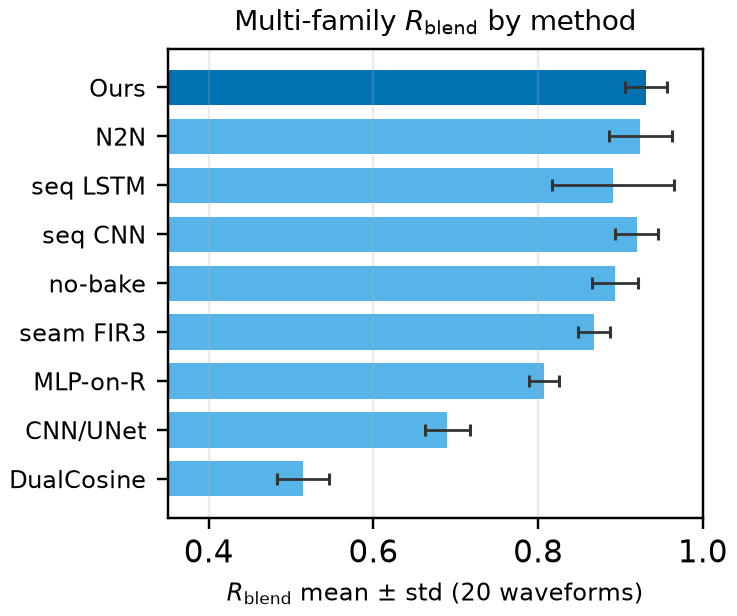
\includegraphics[width=\columnwidth,height=0.28\textheight,keepaspectratio]{figures/fig_sota_method_bars.png}
  \caption{Multi-family mean $R_{\mathrm{blend}}$ by method
  (same $20$-waveform board as Table~\ref{tab:sota-main}).}
  \label{fig:sota-method-bars}
\end{figure}

\begin{figure}[htbp]
  \centering
  \includegraphics[width=\columnwidth,height=0.28\textheight,keepaspectratio]{figures/fig_sota_heatmap.png}
  \caption{Colorblind-safe (\texttt{cividis}) heatmap of mean $R_{\mathrm{blend}}$
  for selected methods $\times$ generative families (2 seeds each). Higher is better.}
  \label{fig:sota-heatmap}
\end{figure}


\subsection{Multi-family and cliff boards}
\label{sec:app-sota-cliff-tables}

Full multi-family ranking (Table~\ref{tab:sota-main}) and hard-cliff strata
(Table~\ref{tab:cliff-strata}) for the Results narrative in
Appendix~\ref{app:secondary-results} and Section~\ref{sec:cliff-strata}.

\begin{table}[htbp]
  \centering
  \caption{Multi-family board (20 waveforms) under $R_{\mathrm{blend}}$ ($\alpha{=}0.7$).
  Core rank columns; SNR/SDR/jump in Table~\ref{tab:sota-main-metrics}.
  $\Delta R$ and ms vs Dual Cosine. N2N/seq seeds \texttt{424242}/\texttt{424243}.}
  \label{tab:sota-main}
  \setlength{\tabcolsep}{3pt}
  \footnotesize
  \begin{tabular}{@{}lrrr@{}}
    \toprule
    Method & $R_{\mathrm{blend}}$ & $\Delta R$ & ms \\
    \midrule
    neural favorite & $0.931\pm0.026$ & ${+}0.417$ & 4.50 \\
    N2N corrupt$\to$corrupt & $0.925\pm0.038$ & ${+}0.410$ & 0.74 \\
    N2N sibling-sup. & $0.924\pm0.035$ & ${+}0.410$ & 0.74 \\
    seq CNN1D & $0.920\pm0.026$ & ${+}0.405$ & 0.53 \\
    no-bake & $0.893\pm0.028$ & ${+}0.379$ & 0.00 \\
    seq LSTM & $0.891\pm0.075$ & ${+}0.376$ & 1.53 \\
    \texttt{seam\_fir3} & $0.868\pm0.019$ & ${+}0.353$ & 0.17 \\
    MLP-on-$R$ & $0.807\pm0.018$ & ${+}0.292$ & 1.76 \\
    CNN/U-Net-on-$R$ & $0.690\pm0.027$ & ${+}0.175$ & 3.08 \\
    DualCosine & $0.514\pm0.032$ & $0$ & 0.98 \\
    soft wide fade & $0.462\pm0.021$ & ${-}0.053$ & 1.87 \\
    \bottomrule
  \end{tabular}
\end{table}

\begin{table}[htbp]
  \centering
  \caption{Multi-family secondary metrics (same board as Table~\ref{tab:sota-main}).}
  \label{tab:sota-main-metrics}
  \setlength{\tabcolsep}{3pt}
  \footnotesize
  \begin{tabular}{@{}lrrr@{}}
    \toprule
    Method & SNR (dB) & SDR (dB) & wrap-jump \\
    \midrule
    neural favorite & $34.6\pm3.2$ & $34.7\pm3.2$ & $0.89\pm0.14$ \\
    N2N corrupt$\to$corrupt & $33.8\pm4.0$ & $33.9\pm4.0$ & $0.89\pm0.15$ \\
    N2N sibling-sup. & $33.9\pm4.1$ & $34.0\pm4.1$ & $0.91\pm0.15$ \\
    seq CNN1D & $32.2\pm3.5$ & $32.4\pm3.5$ & $0.92\pm0.15$ \\
    no-bake & $30.9\pm1.9$ & $31.0\pm1.9$ & $0.91\pm0.15$ \\
    seq LSTM & $32.2\pm5.8$ & $32.4\pm5.8$ & $0.86\pm0.15$ \\
    \texttt{seam\_fir3} & $28.1\pm1.2$ & $28.1\pm1.2$ & $0.46\pm0.08$ \\
    DualCosine & $16.9\pm1.2$ & $16.8\pm1.2$ & $0.32\pm0.05$ \\
    \bottomrule
  \end{tabular}
\end{table}




\begin{table}[htbp]
  \centering
  \caption{Cliff strata on $4{,}096$ holdout tiles under $R_{\mathrm{blend}}$ ($\alpha{=}0.7$).
  Strata by engine wrap-jump ($n$: all $4096$, top25 $1024$, top10 $410$).
  $\pm$ is tile std on the all stratum.}
  \label{tab:cliff-strata}
  \setlength{\tabcolsep}{3pt}
  \footnotesize
  \begin{tabular}{@{}lccc@{}}
    \toprule
    Method & all & top25\% & top10\% \\
    \midrule
    seq LSTM & $0.986\pm0.009$ & 0.989 & 0.990 \\
    N2N sibling-sup. & $0.981\pm0.013$ & 0.985 & 0.985 \\
    N2N corrupt$\to$corrupt & $0.976\pm0.015$ & 0.981 & 0.983 \\
    neural favorite & $0.971\pm0.020$ & 0.978 & 0.978 \\
    seq CNN1D & $0.960\pm0.028$ & 0.969 & 0.970 \\
    no-bake & $0.913\pm0.077$ & 0.929 & 0.922 \\
    \texttt{seam\_fir3} & $0.886\pm0.067$ & 0.870 & 0.869 \\
    DualCosine & $0.525\pm0.239$ & 0.318 & 0.305 \\
    \bottomrule
  \end{tabular}
\end{table}






\subsection{Transfer wrap-protocol status notes}
\label{sec:app-transfer-status}

\begin{table}[htbp]
  \centering
  \caption{Author-method and data-cut status under this wrap-protocol stress test (no invented scores).}
  \label{tab:transfer-sota-status}
  \setlength{\tabcolsep}{3pt}
  \resizebox{\columnwidth}{!}{%
  \begin{adjustbox}{max width=\columnwidth}
\begin{tabular}{@{}lp{0.52\columnwidth}@{}}
    \toprule
    Scope & Note \\
    \midrule
    SeamN2N (ours, N2N-style) & Scored on all seven Table~\ref{tab:transfer-main} boards
      under $R_{\mathrm{blend}}$. Not Lehtinen code \\
    Cycle-GAN (ECG, author) & OOD wrap probe in Table~\ref{tab:transfer-main}
      (MIT-BIH $0.1063$, PTB-XL $0.2105$). Clinical restore $\neq$ wrap residual \\
    BeatDiff (Bedin NeurIPS\,2024) & OOD wrap probe in Table~\ref{tab:transfer-main}
      (MIT-BIH $0.4907$, PTB-XL $0.4933$). Drive prior (not HF).
      Clinical morph prior $\neq$ wrap residual \\
    Paderborn KAt deep (Al~Firdausi CNN) & Trained CNN\_1D\_2L from scratch (not a frozen
      checkpoint) on bearings K001/KA04/KI04/KB23. File-holdout seed \texttt{20260726},
      train seed \texttt{42}, $20$ epochs. 4-class holdout acc $0.8590$ ($n{=}2560$ segs,
      NORMAL/IR/OR/OR+IR). Classifier wrap residual N/A. Arch-reuse wrap bake listed
      in Table~\ref{tab:transfer-main}$^\dagger$.
      Wrap board: Ours $0.9369$ / SeamN2N $0.8421$ / DualCosine $0.4710$ \\
    Expanded PTB-XL & records500 lead-I expanded ($\sim$2k\,$+$\,\texttt{\_hr} records, board $n{=}256$,
      Ours $0.9451$). Multi-lead still out of scope \\
    Real KIT CNC / IEEE PMU & Synthetic pilots only (download walls) \\
    Formal MOS / MUSHRA & Not collected \\
    \bottomrule
  \end{tabular}
\end{adjustbox}%
  }
\end{table}

\subsection{Matched-budget outer-loop comparison}
\label{sec:meta-approaches-results}

Under a $5{,}000$ evaluation budget with LSTM and xLSTM in the searchable bake vocabulary, Table~\ref{tab:meta-approaches} compares Random NAS, Cont.\ CMA-ES, Arch REINFORCE, Aging evolution, TPE Bayes NAS, and my hybrid GA+PPO approach (Ours).
The table reports a matched Deferred D1 re-search under locked $R_{\mathrm{blend}}{+}J$ (mean$\pm$std over three search seeds; artifacts \texttt{meta\_approach\_compare\_v13\_rblend/}).
My hybrid GA+PPO has the top descriptive mean $R_{\mathrm{blend}}$ ($0.9748{\pm}0.0018$; ${\approx}8.4$\,h mean wall).
Aging evolution ranks second ($0.9635{\pm}0.0049$); Arch REINFORCE shows the largest cross-seed variance ($0.9599{\pm}0.0116$).
With only $n{=}3$ matched seeds I do \emph{not} claim formal superiority from non-overlapping uncertainty bands or ANOVA; I use the bake-off to \emph{select} which outer-loop family receives the FitCell-to-plateau budget.
Paired per-search-seed champion deltas (hybrid minus each family) are in the released artifacts in the released artifacts.
Hybrid leads the runner-up (Aging evolution) on all three seeds (mean $\Delta R_{\mathrm{blend}}{=}{+}0.0114$; bootstrap 95\% CI $[0.0064,0.0144]$; Wilson 95\% CI on 3/3 wins $[0.44,1.00]$), but the exact sign-flip test gives $p{=}0.25$ at $n{=}3$ (minimum attainable when all deltas share sign).
Hybrid vs Arch REINFORCE is $2/3$ seed wins ($p{=}0.5$; Wilson 95\% CI $[0.21,0.94]$).
These tests support descriptive selection only.
Only search seed \texttt{1902771841} of the hybrid short-FitCell run clears the frozen holdout Noise2Noise gate under D1 ($R_{\mathrm{blend}}{\approx}0.9766$ vs gate ${\approx}0.9750$).
Mid-search graphs range from about $15$k to $370$k parameters, yet short-FitCell champions stay compact (${\approx}24$k$\pm$2k params across seeds).
Because hybrid had the top mean among the six families, later compute focuses on hybrid-only FitCell-to-plateau (Section~\ref{sec:v14-converge}, Table~\ref{tab:v14-hybrid-converge}).
Noise2Noise is not an outer-loop competitor here (Tables~\ref{tab:n2n-vs-ours},~\ref{tab:sota-main}).
Learning-curve and bar figures use seed \texttt{1902771841} trajectories under the same locked objective.

\input{figures/meta_approaches_table}

\begin{figure}[htbp]
  \centering
  \includegraphics[width=\columnwidth,height=0.28\textheight,keepaspectratio]{figures/meta_approach_bars.png}
  \caption{Matched 5,000-evaluation search methods under locked $R_{\mathrm{blend}}{+}J$ (seed \texttt{1902771841}).
  Table~\ref{tab:meta-approaches} reports mean$\pm$std across three search seeds.
  Dashed line: Dual Cosine on the same runner.}
  \label{fig:meta-approach-bars}
\end{figure}

\begin{figure}[htbp]
  \centering
  \includegraphics[width=\columnwidth,height=0.28\textheight,keepaspectratio]{figures/fig_meta_approach_compare.png}
  \caption{Champion $R_{\mathrm{blend}}$ over a matched 5,000-evaluation budget (Deferred D1 complete; seed \texttt{1902771841}).
  Dashed line: Dual Cosine.}
  \label{fig:meta-approach-compare}
\end{figure}

\subsection{Ablations and compute}
\label{sec:ablation-compute}

Table~\ref{tab:ablation} answers two narrow questions, not a full factorial re-search of Table~\ref{tab:meta-approaches}.
\textbf{Left column:} within one recorded hybrid history under the superseded prolonged-$R$ search metric, what was the best freeze tagged by outer-loop branch (PPO/GA/PBT/\ldots) at the $5$k gate?
These are branch labels in a single run, not separately fitted champions, so they mainly show that no single branch monopolizes the trajectory.
\textbf{Right column:} isolated $150$-iteration \texttt{ablate-*} restarts (seed \texttt{1902771841}) whose final cells are re-scored under locked $R_{\mathrm{blend}}$.
They probe whether dropping GA or PPO collapses residual under a short budget; they are \emph{not} matched-$5$k competitors and must not overwrite Table~\ref{tab:meta-approaches}.
\paragraph{How to read Table~\ref{tab:ablation}.}
Left-column values are close to each other (${\approx}0.987$--$0.991$ prolonged $R$): in that single history, branch tags do not identify a unique winner, so I do not treat ``GA-only freeze'' as proof that GA alone suffices under locked $R_{\mathrm{blend}}$.
Right-column short restarts under $R_{\mathrm{blend}}$ stay far below the matched-$5$k hybrid mean ($0.9748$) and the converge seed ($0.9912$) because the budget is only $150$ iterations with short FitCell, they are sensitivity checks, not leaderboard rows.
The matched comparison that drives method choice remains Table~\ref{tab:meta-approaches}.
Table~\ref{tab:compute} summarizes campaign compute (historical prolonged-$R$ search).

\begin{table}[htbp]
  \centering
  \caption{Ablations (interpret narrowly).
    Left: best prolonged $R$ by branch label in one hybrid history (final iteration ${\approx}6{,}922$; superseded search metric; not separate fits).
    Right: isolated 150-iteration \texttt{ablate-*} final champions re-scored under $R_{\mathrm{blend}}$ ($\alpha{=}0.7$; seed \texttt{1902771841}).
    Full $5{,}000$-evaluation $R_{\mathrm{blend}}$ branch re-search is reported in Section~\ref{sec:ablation-def}; use Table~\ref{tab:meta-approaches} for matched outer-loop comparison.}
  \label{tab:ablation}
  \setlength{\tabcolsep}{3pt}
  \begin{adjustbox}{max width=\columnwidth}
  \begin{tabular}{@{}lrr@{}}
    \toprule
    Config & Prolonged $R$ freeze & 150-it $R_{\mathrm{blend}}$ \\
    \midrule
    Full hybrid & 0.99093 & 0.92710 \\
    GA-only & 0.99016 & 0.94168 \\
    PBT (search branch) & 0.99012 & n/a \\
    PPO-only & 0.98924 & 0.94405 \\
    GA+PPO & n/a & 0.94478 \\
    Combined branch & 0.98854 & n/a \\
    NAS branch & 0.98677 & n/a \\
    Dual Cosine (runner) & 0.81658 & ${\approx}0.539$ \\
    \bottomrule
  \end{tabular}
\end{adjustbox}
\end{table}

\begin{table}[htbp]
  \centering
  \caption{Compute budget for the reported 5,000-evaluation search run (RTX~3090, search seed \texttt{1902771841}; prolonged-$R$ objective).
    Final champion $R$ below is the historical prolonged freeze, not $R_{\mathrm{blend}}$.}
  \label{tab:compute}
  \setlength{\tabcolsep}{3pt}
  \begin{adjustbox}{max width=\columnwidth}
\begin{tabular}{@{}lr@{}}
    \toprule
    Item & Value \\
    \midrule
    GPU & NVIDIA GeForce RTX 3090 \\
    Elapsed wall time & ${\approx}7.92$\,h \\
    Clean iterations / arch evals & ${\approx}6{,}922$ \\
    Population size & 12 \\
    Final champion prolonged $R$ & 0.99093 \\
    Dual Cosine baseline (runner, prolonged) & 0.81658 \\
    Peak VRAM (replay) & ${\approx}3.29$\,GiB \\
    \bottomrule
  \end{tabular}
\end{adjustbox}
\end{table}

\subsection{Hyperparameter sensitivity}
\label{para:hp-sensitivity}
One-at-a-time $\pm 50\%$ probe of Table~\ref{tab:hyperparams} knobs at $500$ outer iterations (seed \texttt{1902771841}).
\textbf{Pilot / diagnostic only} (not a $5$k re-search).
Default champion $R{\approx}0.9888$. The largest $|\Delta R|$ among OAT arms is ${\approx}0.0123$ (50\% lower learning rate).
All eleven configurations completed ($1$ default plus ten $\pm 50\%$ one-at-a-time perturbations), each running $500/500$ outer iterations, ``$11/11$'' counts finished configs, not an $11/11$ win rate at 50\%.

\input{figures/tab_meta_hp_sensitivity}

\begin{figure}[htbp]
  \centering
  \includegraphics[width=\linewidth,height=0.28\textheight,keepaspectratio]{figures/fig_meta_hp_sensitivity.png}
  \caption{One-at-a-time $\pm 50\%$ HP sensitivity of hybrid champion $R$ at 500 iterations. Blue bar: Table~\ref{tab:hyperparams} default.}
  \label{fig:hp-sensitivity}
\end{figure}

\subsection{Transfer inference latency}
\label{sec:transfer-latency-app}
Table~\ref{tab:transfer-latency} and Figure~\ref{fig:signal-heal-transfer-latency} pair with the prolonged-$R$ transfer board (Table~\ref{tab:transfer-main}).
N2N latency uses the wavetable checkpoint zero-shot. Domain-trained N2N quality scores are in Table~\ref{tab:transfer-main}.

\begin{table}[htbp]
  \centering
  \caption{Transfer-domain inference latency (ms/batch). Batch=64, CUDA.}
  \label{tab:transfer-latency}
  \setlength{\tabcolsep}{4pt}
  \begin{adjustbox}{max width=\columnwidth}
\begin{tabular}{@{}lrrrrrr@{}}
    \toprule
    Method & CWRU & MFPT & MIT-BIH & PTB-XL & CNC & PMU \\
    \midrule
    no-bake & 0.26 & 0.26 & 0.27 & 0.27 & 0.28 & 0.26 \\
    Dual Cosine & 1.10 & 1.11 & 1.12 & 1.14 & 1.15 & 1.14 \\
    Ours (hybrid) & 3.92 & 6.61 & 2.87 & 1.67 & 1.69 & 1.67 \\
    N2N (WT to domain) & 0.95 & 0.99 & 0.98 & 0.97 & 0.98 & 0.97 \\
    \bottomrule
  \end{tabular}
\end{adjustbox}
\end{table}

\begin{figure}[htbp]
  \centering
  \includegraphics[width=\columnwidth,height=0.28\textheight,keepaspectratio]{figures/fig_signal_heal_transfer_latency.png}
  \caption{Transfer-domain inference latency (ms/batch). N2N is wavetable-trained zero-shot when available.}
  \label{fig:signal-heal-transfer-latency}
\end{figure}

\subsection{Search-monitor figures}
\label{sec:search-monitor-figs}

\begin{figure}[htbp]
  \centering
  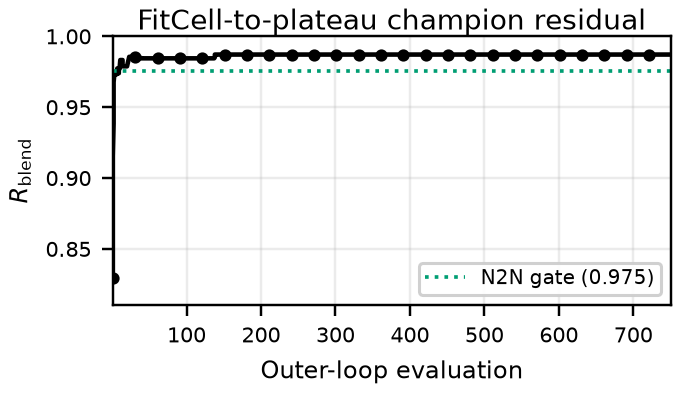
\includegraphics[width=\columnwidth,height=0.28\textheight,keepaspectratio]{figures/champ_residual_vs_iter.png}
  \caption{FitCell-to-plateau champion $R_{\mathrm{blend}}$ vs.\ outer-loop evaluation
  (seed \texttt{1902771841}; y-axis zoomed to the high-$R$ regime with Noise2Noise gate marked).}
  \label{fig:champ-residual}
\end{figure}

\begin{figure}[htbp]
  \centering
  \includegraphics[width=\columnwidth,height=0.28\textheight,keepaspectratio]{figures/branch_bests_vs_iter.png}
  \caption{Best residual by search branch (earlier search monitor freeze; search-trace artifact).}
  \label{fig:branch-bests}
\end{figure}

\begin{figure}[htbp]
  \centering
  \includegraphics[width=\columnwidth,height=0.28\textheight,keepaspectratio]{figures/search_panel.png}
  \caption{Search progress: champion $R$ (top) and branch bests (bottom).}
  \label{fig:search-panel}
\end{figure}

\begin{figure}[htbp]
  \centering
  \includegraphics[width=\columnwidth,height=0.28\textheight,keepaspectratio]{figures/residual_by_branch.png}
  \caption{Per-trial residual by branch with champion trajectory overlaid.}
  \label{fig:residual-branch}
\end{figure}

\begin{figure}[htbp]
  \centering
  \includegraphics[width=\columnwidth,height=0.28\textheight,keepaspectratio]{figures/champion_timeline.png}
  \caption{Champion updates (earlier search monitor freeze; search-trace artifact).}
  \label{fig:champ-timeline}
\end{figure}

\subsection{Inference and classical diagnostic plots}
\label{sec:app-inference-diags}

\begin{figure}[htbp]
  \centering
  \includegraphics[width=\columnwidth,height=0.28\textheight,keepaspectratio]{figures/fig_inference_vs_residual.png}
  \caption{High-$R$ fitted operators: residual vs CUDA latency. Star: favorite.}
  \label{fig:inference-pareto}
\end{figure}

\begin{figure}[htbp]
  \centering
  \includegraphics[width=\columnwidth,height=0.28\textheight,keepaspectratio]{figures/fig_inference_latency_bars.png}
  \caption{Inference latency for high-$R$ fitted models (CUDA, batch 64).}
  \label{fig:inference-bars}
\end{figure}

\begin{figure}[htbp]
  \centering
  \includegraphics[width=\columnwidth,height=0.28\textheight,keepaspectratio]{figures/fig_classical_vs_ai_scatter.png}
  \caption{Canonical holdout: classical methods and favorite in the $R$ vs ms/batch plane.}
  \label{fig:classical-vs-ai-scatter}
\end{figure}

\begin{figure}[htbp]
  \centering
  \includegraphics[width=\columnwidth,height=0.28\textheight,keepaspectratio]{figures/fig_classical_vs_ai_bars.png}
  \caption{Canonical holdout ranking on $R_{\mathrm{blend}}$ (left) and latency (right).}
  \label{fig:classical-vs-ai-bars}
\end{figure}

\section{Secondary wavetable results}
\label{app:secondary-results}

Moved from the main Results section to shorten the conference-length reading path.
Primary holdout, meta-compare, and converge claims remain in Section~\ref{sec:results}.

\paragraph{Superseded whole-curve freezes.}
Whole-curve prolonged-$R$ freezes ($R{\approx}0.991$ vs DualCosine ${\approx}0.825$) are not current results.
Selection and published comparison under v10.1 use $R_{\mathrm{blend}}{+}J$ with Noise2Noise as the primary neural baseline.

\subsection{Which families stay hard}
\label{sec:family-hardness}
On the fitted DenoiseOpt $100{,}000$-cycle bench, denoise score $D$ is lowest for \texttt{nonlinear} ($D\approx 0.39$) and \texttt{combo} ($D\approx 0.40$), then \texttt{triple\_mix} / \texttt{extreme\_overlay} ($D\approx 0.51$--$0.52$), while \texttt{harmonic\_fft} and \texttt{am\_fm} sit near $D\approx 0.69$--$0.70$.
Lit-combo champion family stress (prolonged residual) similarly ranks \texttt{open\_wrap\_bias} ($R\approx 0.83$) and \texttt{extreme\_overlay} / \texttt{combo} ($R\approx 0.88$--$0.89$) below \texttt{harmonic\_fft} ($R\approx 0.95$).
Hard sounds recur.

\paragraph{Superseded $5$k-gate freeze.}
At the reported $5$k-gate search freeze ($\approx 6{,}922$ clean iterations, $\approx 7.9$\,h on RTX~3090) the champion residual was $R\approx 0.99093$ with DualCosine $\approx 0.81658$ on the CUDA search runner ($\Delta R\approx{+}0.174$).
That freeze optimized whole-curve prolonged $R$.
It is superseded by $R_{\mathrm{blend}}$ for v10.1 selection.
Monitoring plots below come from that older freeze and should be read as search-trace artifacts, not as locked-protocol scores.

\subsection{Inference latency at matched score}
\label{sec:inference-latency}
Across the prior high-prolonged-$R$ fitted operators, I re-timed CUDA forward passes under locked $R_{\mathrm{blend}}$ (batch 64).
Live $R_{\mathrm{blend}}$ spreads more than the old prolonged band: the max-$R_{\mathrm{blend}}$ model is
\texttt{champion\_iter\_000265} ($R_{\mathrm{blend}}{\approx}0.9769$, $\approx 6.53$\,ms/batch, $\approx 94$k params).
The compact historically favorite \texttt{iter\_000235} remains lowest-latency among the top-5 distinct topologies
($R_{\mathrm{blend}}{\approx}0.9749$, $\approx 3.42$\,ms/batch, $\approx 37$k params).
Selection rule: maximize live $R_{\mathrm{blend}}$, then minimize latency inside $R\ge R_{\max}-5\cdot10^{-4}$.

\subsection{Top-5 architectures}
\label{sec:top5-arch}
Table~\ref{tab:top5} ranks five distinct fitted bake graphs from the CUDA inference bench
(\codehref{https://github.com/reeldemo/denoise-opt}{inference data}, batch 64), preferring live $R_{\mathrm{blend}}$ first and latency on ties,
and skipping near-duplicate copies of the same topology signature.

\begin{table}[htbp]
  \centering
  \caption{Top-5 distinct fitted architectures on the CUDA inference bench (batch 64) under $R_{\mathrm{blend}}$ ($\alpha{=}0.7$).
  $R_{\mathrm{saved}}$ is the checkpoint hint (often prolonged $R$); $R_{\mathrm{live}}$ is measured $R_{\mathrm{blend}}$.
  *Max-$R_{\mathrm{blend}}$ (also sole member of the $R\ge R_{\max}-5\cdot10^{-4}$ band here).}
  \label{tab:top5}
  \setlength{\tabcolsep}{3pt}
  \begin{adjustbox}{max width=\columnwidth}
\begin{tabular}{@{}lrrrr@{}}
    \toprule
    Tag & $R_{\mathrm{saved}}$ & $R_{\mathrm{live}}$ & ms/batch & params \\
    \midrule
    \texttt{iter\_000265}* & 0.9906 & 0.9769 & 6.53 & 93\,566 \\
    \texttt{iter\_000140} & 0.9906 & 0.9762 & 7.16 & 104\,484 \\
    \texttt{iter\_000133} & 0.9908 & 0.9752 & 7.16 & 104\,484 \\
    \texttt{iter\_000229} & 0.9909 & 0.9751 & 7.56 & 100\,500 \\
    \texttt{iter\_000235} & 0.9910 & 0.9749 & 3.42 & 37\,489 \\
    \bottomrule
  \end{tabular}
\end{adjustbox}\\[0.4em]
  {\footnotesize *Favorite under maximize-$R_{\mathrm{blend}}$ then latency. Compact \texttt{iter\_000235} is still the latency floor in this top-5.}
\end{table}

\label{sec:classical-vs-favorite}
Table~\ref{tab:canonical-methods} scores the classical (non-AI) bake set (no-bake, DualCosine, and \texttt{seam\_fir3}) plus the locked v10.1 hybrid favorite on the frozen corpus of Section~\ref{sec:dataset} (CUDA, batch 64, seed \texttt{20260719}) under $R_{\mathrm{blend}}$.
DualCosine reaches $R_{\mathrm{blend}}\approx 0.541$ ($\approx 1.66$\,ms/batch).
Active classical \texttt{seam\_fir3} reaches $0.884$ / $\approx 1.11$\,ms/batch ($0.888\pm0.009$ over five seeds).
No-bake (passthrough) scores $0.914$ ($0.917\pm0.009$).
The hybrid favorite reaches $0.970$ ($0.971\pm0.001$ over five seeds) at $\approx 5.99$\,ms/batch:
$\Delta R_{\mathrm{blend}} \approx {+}0.056$ vs no-bake and $\approx {+}0.429$ vs DualCosine.
Noise2Noise on the multi-family matrix is Appendix Table~\ref{tab:sota-main}. The four-board gate is Table~\ref{tab:n2n-vs-ours}.

\begin{table}[htbp]
  \centering
  \caption{Canonical holdout under $R_{\mathrm{blend}}$ ($\alpha{=}0.7$; seed \texttt{20260719}). Mean$\pm$std over five seeds. No-bake $=$ unrepaired engine. Favorite $=$ locked v10.1 hybrid champ.}
  \label{tab:canonical-methods}
  \setlength{\tabcolsep}{6pt}
  \begin{adjustbox}{max width=\columnwidth}
\begin{tabular}{@{}lrrr@{}}
    \toprule
    Method & $R_{\mathrm{blend}}$ & $R_{\mathrm{blend}}$ (5-seed) & ms/batch \\
    \midrule
    neural favorite & 0.9697 & $0.9708\pm0.0012$ & 5.99 \\
    no-bake (passthrough) & 0.9142 & $0.9166\pm0.0090$ & 1.06 \\
    \texttt{seam\_fir3} & 0.8842 & $0.8879\pm0.0087$ & 1.11 \\
    classic quadratic & 0.5742 & $0.5727\pm0.0318$ & 2.07 \\
    DualCosine & 0.5409 & $0.5420\pm0.0342$ & 1.66 \\
    cosine fade & 0.5409 & $0.5420\pm0.0342$ & 1.87 \\
    crossfade & 0.5310 & $0.5273\pm0.0311$ & 1.86 \\
    hann blend & 0.5197 & $0.5214\pm0.0337$ & 1.05 \\
    soft wide fade & 0.4828 & $0.4803\pm0.0258$ & 2.85 \\
    detrend & 0.3437 & $0.3453\pm0.0399$ & 0.96 \\
    ensemble detrend{+}DC{+}FIR & 0.3126 & $0.3100\pm0.0421$ & 2.00 \\
    \bottomrule
  \end{tabular}
\end{adjustbox}
\end{table}



\subsection{Multi-family comparison}
\label{sec:sota-main}

Does the locked hybrid favorite beat the classical non-AI board (no-bake, DualCosine, FIR, fades),
fixed MLP/CNN baselines, \emph{and} Noise2Noise across twenty generative families under $R_{\mathrm{blend}}$?
Appendix Table~\ref{tab:sota-main} reports mean$\pm$std over the 20-waveform multi-family set (Section~\ref{sec:dataset}) from the \codehref{https://github.com/reeldemo/denoise-opt}{SOTA matrix}.
Appendix Figures~\ref{fig:sota-heatmap}--\ref{fig:sota-method-bars} plot the same ranking.
Primary reading is absolute $R_{\mathrm{blend}}$ rank:
Ours $0.934$, corrupt$\to$corrupt N2N $0.931$, seq CNN $0.920$, no-bake $0.893$,
\texttt{seam\_fir3} $0.868$, DualCosine $0.514$
(aligned with Table~\ref{tab:n2n-vs-ours} multifamily).
Fixed MLP-on-$R$ and CNN/U-Net-lite-on-$R$ (no outer NAS) sit between DualCosine and the neural rows.
Vs DualCosine on the same $n{=}20$ waveforms, a paired Wilcoxon signed-rank test (normal approx.) gives $W{=}0$, $p{\approx}8.9{\times}10^{-5}$, mean $\Delta R_{\mathrm{blend}}{=}{+}0.417$ (bootstrap 95\% CI $[0.398,0.435]$); treat this as a small-$n$ exploratory check, not a powered multi-study claim.
Vs no-bake the multifamily mean gap is $\approx{+}0.038$.
Vs corrupt$\to$corrupt N2N the mean-of-means gap is $\approx{+}0.003$ with sign-test parity (mean win fraction $0.47$ across five eval seeds; Section~\ref{sec:n2n-vs-ours-boards}), overlapping std bands must not be read as Ours superiority.

\paragraph{Cliff stratification (full).}
Main-text summary: Section~\ref{sec:cliff-strata}.
Appendix Table~\ref{tab:cliff-strata} stratifies the $4{,}096$-tile holdout by wrap-jump percentiles.

\subsection{Noise2Noise and sequence baselines}
\label{sec:n2n-baselines}

How does DenoiseOpt compare to true Noise2Noise-style and lightweight seq restorers on the same generator under $R_{\mathrm{blend}}$?
Primary corrupt$\to$corrupt N2N (train seed \texttt{424242}) reaches holdout $R_{\mathrm{blend}}\approx 0.975$ (Table~\ref{tab:n2n-vs-ours}), above the hybrid favorite ($0.970$).
On the $4{,}096$-tile cliff draw, sibling-supervised N2N reaches $0.981$ and seq LSTM $0.986$ (Appendix Table~\ref{tab:cliff-strata}).
Holdout tiles never enter training.
Classical DualCosine / \texttt{seam\_fir3} remain in Appendix Table~\ref{tab:cliff-strata}.
Figure~\ref{fig:n2n-vs-ours} plots the four-board $R_{\mathrm{blend}}$ comparison.

\begin{figure}[t]
  \centering
  \includegraphics[width=\columnwidth]{figures/fig_n2n_vs_ours_bars.png}
  \caption{Canonical holdout $R_{\mathrm{blend}}$: N2N and seq baselines vs Ours (locked hybrid).
    Train seeds \texttt{424242}/\texttt{424243} are disjoint from holdout \texttt{20260719}.}
  \label{fig:n2n-vs-ours}
\end{figure}



\subsection{Factory exports and AKWF cycles}
\label{sec:real-wt}

Does the wrap protocol transfer beyond synthetic sine cliffs onto true exports and third-party OA cycles?
Table~\ref{tab:real-wt} scores ReelSynth-exported factory periods (primary realism) and Adventure Kid Waveforms (AKWF) CC0 single-cycle WAVs (secondary) after close-seam idealization and the same open-wrap cliff, under $R_{\mathrm{blend}}$.
Procedural stand-ins are demoted to tertiary smoke and no longer carry the primary realism claim.
On exported factory periods the favorite ($R_{\mathrm{blend}}{\approx}0.699$) trails no-bake / FIR / poly / N2N while still beating Dual Cosine ($0.589$).
On AKWF OA cycles the favorite ($0.679$) trails no-bake / N2N and scores above Dual Cosine ($0.424$) on mean $R_{\mathrm{blend}}$ (single-board means; not a listening claim).
Export gaps are listed in Section~\ref{sec:limitations}.

\begin{table}[t]
  \centering
  \caption{Wavetable-native wrap protocol under $R_{\mathrm{blend}}$ ($\alpha{=}0.7$). Close-seam ideal $\to$ open-wrap cliff (seed \texttt{20260719}). Primary = ReelSynth export. Secondary = AKWF CC0 files.}
  \label{tab:real-wt}
  \setlength{\tabcolsep}{6pt}
  \begin{adjustbox}{max width=\columnwidth}
\begin{tabular}{@{}lrr@{}}
    \toprule
    Method & Export & AKWF OA \\
    \midrule
    \texttt{seam\_fir3} & 0.863 & 0.725 \\
    poly seam ($d{=}3$) & 0.846 & 0.696 \\
    no-bake & 0.845 & 0.702 \\
    endpoint-pin (mean) & 0.792 & 0.745 \\
    N2N corrupt$\to$corrupt & 0.771 & 0.731 \\
    seq CNN1D & 0.706 & 0.677 \\
    neural favorite & 0.699 & 0.679 \\
    DualCosine & 0.589 & 0.424 \\
    seq LSTM & 0.628 & 0.579 \\
    \bottomrule
  \end{tabular}
\end{adjustbox}
\end{table}

\subsection{Polynomial baseline and endpoint pinning}
\label{sec:poly-jump}

Does a cheap classical poly fitter close the residual, and does endpoint pinning show the wrap-jump vs $R_{\mathrm{blend}}$ tradeoff?
A seam-local degree-3 polynomial fitter (no learning) reaches canonical $R_{\mathrm{blend}}\approx 0.917$ (slightly above no-bake $0.914$) with wrap-jump essentially unchanged (\codehref{https://github.com/reeldemo/denoise-opt}{polynomial results}).
SSM seq models are deferred. The LSTM remains the supervised seq ceiling.
An endpoint-pin control (\codehref{https://github.com/reeldemo/denoise-opt}{pinning results}) drives wrap-jump to $0$ on all / hard subsets while dropping $R_{\mathrm{blend}}$ (all $0.733$, hard $0.597$).
Methods that zero wrap-jump are not the same objective as $R_{\mathrm{blend}}$ (Limitations).

\subsection{Classical virtual-analog seam repairs}
\label{sec:va-seam-baselines}

Do the cited VA antialias tools~\cite{stilson1996,nam2009polyblep,esqueda2016blamp} beat DualCosine on $R_{\mathrm{blend}}$ when applied as cycle-local seam residuals?

\paragraph{What each operator changes.}
Figure~\ref{fig:va-seam-techniques} shows the family on one high-wrap sine{+}cliff tile (same seed and tile as Figure~\ref{fig:intro-sine}).
\textbf{BLIT/BLEP} (Stilson/Smith lineage) treats the wrap as a value step.
It subtracts a band-limited step residual (here a raised-cosine BLEP-family lobe scaled by the measured wrap jump) so the tiled click spectrum is softened near the seam.
\textbf{PolyBLEP} (Nam et al.) is a cheap polynomial surrogate of that step residual with fractional-delay support near phase wrap.
It edits only a few samples on each side of the discontinuity.
\textbf{BLAMP}~\cite{esqueda2016blamp} corrects a slope or corner jump (discontinuity in the first derivative), which matters for triangles, rectification, and hard clipping.
On a pure value cliff the slope jump is small, so BLAMP is nearly a no-bake passthrough.
\textbf{DualCosine} (my classical bake baseline) fades both ends of the stored period with raised-cosine windows.
It does not insert a BLEP-style residual.
It trades wrap energy for a wide end-fade distortion that $R_{\mathrm{blend}}$ penalizes on hard cliffs.

\paragraph{Scores.}
Table~\ref{tab:va-seam-blep} reports batch means from the \codehref{https://github.com/reeldemo/denoise-opt}{VA results} (seed \texttt{20260719}, batch 64) under $R_{\mathrm{blend}}$.
Code is in the \codehref{https://github.com/reeldemo/reelsynth}{ReelSynth repository}: PolyBLEP matches \texttt{osc::va::poly\_blep}, BLIT/BLEP uses a raised-cosine step residual, and BLAMP applies a polyBLAMP lobe to the wrap slope jump.
PolyBLEP reaches mean $R_{\mathrm{blend}}\approx 0.795$ ($\Delta\approx{+}0.254$ vs DualCosine) but trails no-bake / \texttt{seam\_fir3}.
BLIT/BLEP nearly zeros wrap-jump ($0.004$), yet mean $R_{\mathrm{blend}}$ falls to $0.632$ and hard cliffs collapse to $0.351$.
BLAMP stays near no-bake on this value-cliff geometry (mean $0.914$).
On the annotated severe tile in Figure~\ref{fig:va-seam-techniques}, tile $R_{\mathrm{blend}}$ is lower still (PolyBLEP $\approx 0.726$, BLIT/BLEP $\approx 0.385$, Dual Cosine $0.300$, BLAMP $\approx$ engine).
I score these classical tools, not only cite them: they beat DualCosine on mean $R_{\mathrm{blend}}$ in places, and none matches the locked hybrid favorite on holdout $R_{\mathrm{blend}}$.

\begin{figure}[t]
  \centering
  \includegraphics[width=\columnwidth]{figures/fig_va_seam_techniques.png}
  \caption{Classical VA seam techniques on one cracked sine{+}cliff tile
  (seed~\texttt{20260719}, tile~46).
  (a)~ideal; (b)~cracked engine; (c)~BLIT/BLEP; (d)~PolyBLEP; (e)~BLAMP; (f)~DualCosine.
  Batch means: Table~\ref{tab:va-seam-blep}.}
  \label{fig:va-seam-techniques}
\end{figure}

\begin{table}[t]
  \centering
  \caption{Classical VA seam repairs under $R_{\mathrm{blend}}$ ($\alpha{=}0.7$; seed \texttt{20260719}).
  Holdout $R_{\mathrm{blend}}$, seam-local edge RMSE, cliff top-10\% $R_{\mathrm{blend}}$, multi-family mean.}
  \label{tab:va-seam-blep}
  \setlength{\tabcolsep}{3pt}
  \footnotesize
  \begin{tabular}{@{}lcccc@{}}
    \toprule
    Method & $R$ & edge & top10 & multi \\
    \midrule
    BLAMP & 0.914 & 0.080 & 0.922 & 0.893 \\
    no-bake & 0.914 & 0.080 & 0.922 & 0.893 \\
    \texttt{seam\_fir3} & 0.884 & 0.112 & 0.869 & 0.868 \\
    PolyBLEP & 0.795 & 0.205 & 0.690 & 0.784 \\
    BLIT/BLEP & 0.632 & 0.365 & 0.351 & 0.612 \\
    DualCosine & 0.541 & 0.506 & 0.305 & 0.514 \\
    \bottomrule
  \end{tabular}\\[0.35em]
  {\footnotesize Latency (CUDA): PolyBLEP ${\approx}0.87$\,ms/batch, DualCosine ${\approx}1.46$, BLIT/BLEP ${\approx}71$, BLAMP ${\approx}20$.}
\end{table}





\subsection{When search helps vs classical methods}
\label{sec:transfer}

Per-cycle $\Delta R$ on export, AKWF, Rust \texttt{sound\_bench}, and sine{+}cliff holdout
(\codehref{https://github.com/reeldemo/denoise-opt}{transfer results}):
favorite win-rate vs Dual Cosine is high on sine cliffs ($1.00$) and AKWF ($0.88$), and moderate on export ($0.64$) / Rust ($0.75$).
Win-rate vs no-bake is high only on sine cliffs ($0.92$) and collapses on export ($0.24$) / Rust ($0.20$).
Search value is highest on hard cliffs and when compact bake graphs are needed without engine$\to$ideal labels at search time.
Export / Rust gaps vs no-bake are listed in Section~\ref{sec:limitations}.

\subsection{Transfer to Rust engine tiles}
\label{sec:rust-bench}

Table~\ref{tab:rust-bench} scores the Python-trained favorite on 20 Rust-exported tiles under $R_{\mathrm{blend}}$ (\textbf{pilot / diagnostic}; $n{=}20$).
The favorite shows mean $\Delta R_{\mathrm{blend}}{+}0.082$ vs Dual Cosine, but the signed-rank test is not significant at $\alpha{=}0.05$ ($p{\approx}0.30$); do not read the mean gap as superiority.
The primary SOTA claim remains the Python multi-family matrix.

\begin{table}[t]
  \centering
  \caption{Rust \texttt{sound\_bench} transfer (\textbf{pilot / diagnostic}, $n{=}20$ tiles) under $R_{\mathrm{blend}}$ ($\alpha{=}0.7$).
  $\Delta$ is vs Dual Cosine. Absolute scores trail no-bake and \texttt{seam\_fir3}.}
  \label{tab:rust-bench}
  \setlength{\tabcolsep}{6pt}
  \begin{adjustbox}{max width=\columnwidth}
\begin{tabular}{@{}lrr@{}}
    \toprule
    Method & $R_{\mathrm{blend}}$ & $\Delta$ vs DC \\
    \midrule
    no-bake & $0.846\pm0.171$ & ${+}0.422$ \\
    \texttt{seam\_fir3} & $0.751\pm0.157$ & ${+}0.327$ \\
    neural favorite & $0.506\pm0.236$ & ${+}0.082$ \\
    classic quadratic & $0.474\pm0.186$ & ${+}0.050$ \\
    Dual Cosine / cosine fade & $0.424\pm0.187$ & $0$ \\
    \bottomrule
  \end{tabular}
\end{adjustbox}
\end{table}

\paragraph{Paired statistics on the five-seed holdout and multifamily boards.}
Computed by the repository script in the released artifacts (output the repository script).
Hybrid minus frozen Noise2Noise on the five-seed holdout: mean $\Delta R_{\mathrm{blend}}={-}0.0060$ (bootstrap 95\% CI $[{-}0.0066,{-}0.0053]$; 0/5 seed wins, Wilson 95\% CI $[0.00,0.43]$; exact sign-flip $p=0.0625$, the minimum attainable at $n{=}5$; Hedges $g_z={-}5.6$).
Hybrid minus DualCosine: $\Delta={+}0.429$ ($[0.402,0.462]$; 5/5 wins, Wilson CI $[0.57,1.00]$; $p=0.0625$).
On the 20 multifamily boards, hybrid minus Noise2Noise is $\Delta={+}0.0030$ ($[{-}0.006,0.013]$; 10/20 wins, Wilson CI $[0.30,0.70]$; exact permutation $p=0.55$; $g_z=0.13$): no detectable difference (CIs overlap zero).
These tests are exploratory; $n{=}5$ seeds cannot reach $p<0.05$ under an exact two-sided paired test, so a powered claim needs $\ge 6$ holdout seeds.

\begin{figure*}[t]
  \centering
  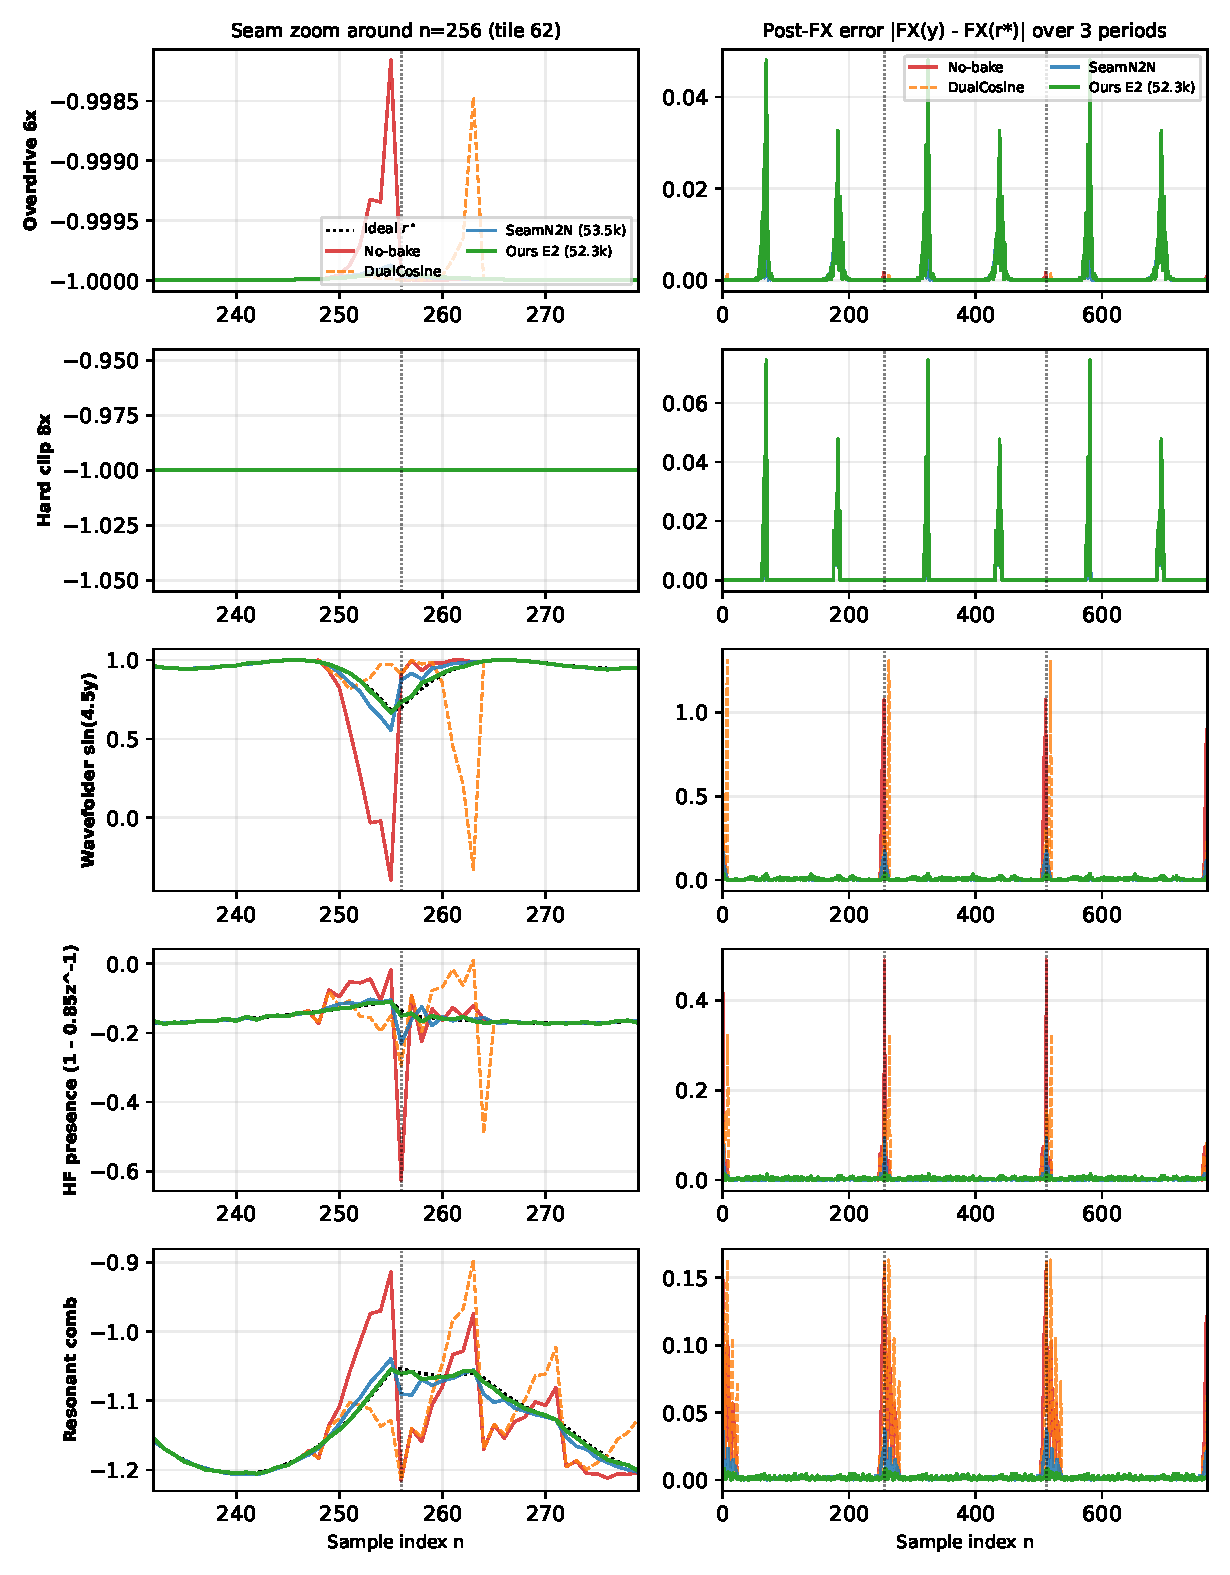
\includegraphics[width=0.92\textwidth]{figures/fig_fx_suite_repair.pdf}
  \caption{Downstream FX stress-test visualization on holdout tile~62 (seed~\texttt{20260719}) across five effects: $6{\times}$ overdrive, $8{\times}$ hard clipping, $\sin(4.5y)$ wavefolder, HF presence ($1{-}0.85z^{-1}$), and resonant comb.
    Left: seam zoom around $n{=}256$. Right: post-FX waveform error $|\mathrm{FX}(y){-}\mathrm{FX}(r^{\star})|$ over three looped periods. Dual Cosine and SeamN2N leave seam error bursts under downstream FX, while Ours E2 (\texttt{2026072701}, $52.3$k) remains flat.}
  \label{fig:fx-suite-repair}
\end{figure*}

\begin{figure*}[t]
  \centering
  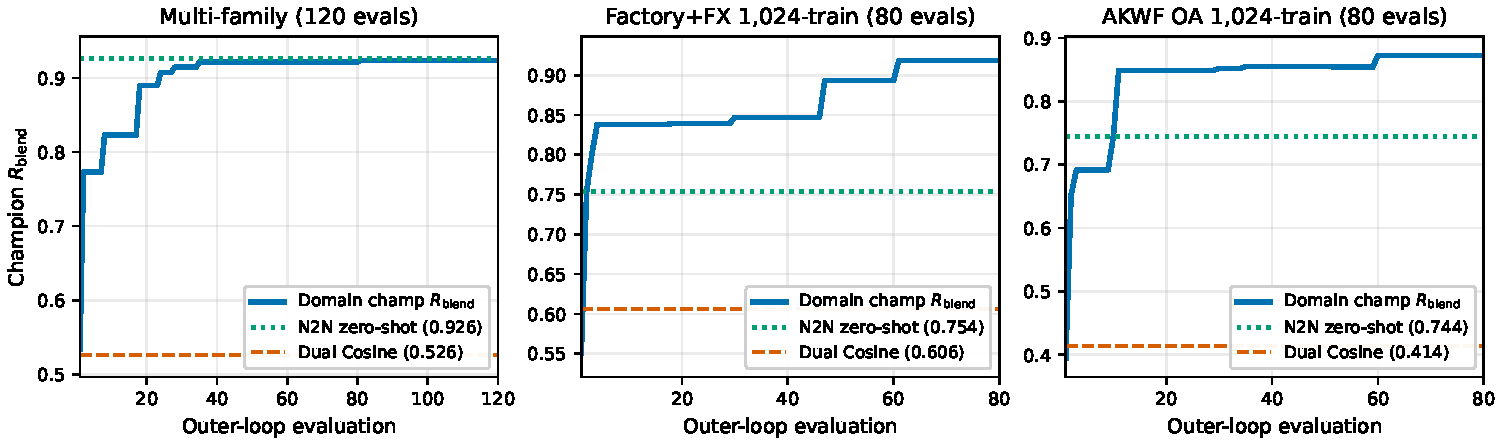
\includegraphics[width=0.95\textwidth]{figures/fig_domain_search_curves.pdf}
  \caption{Per-board DenoiseOpt (\texttt{hybrid\_lstm}) domain-search learning curves corresponding to Table~\ref{tab:n2n-vs-ours}.
    Left: Multi-family ($120$ evals, $120$ FitCell steps). Center: Factory+FX ($1{,}024$-cycle train split, $80$ evals, $100$ FitCell steps; held-out $256$-cycle $R_{\mathrm{blend}}{=}0.911$). Right: AKWF OA ($1{,}024$-cycle train split, $80$ evals, $100$ FitCell steps; held-out $256$-cycle $R_{\mathrm{blend}}{=}0.874$). Dotted/dashed lines show zero-shot \texttt{SeamN2N} and Dual Cosine on the same held-out splits.}
  \label{fig:domain-search-curves}
\end{figure*}

\begin{figure*}[t]
  \centering
  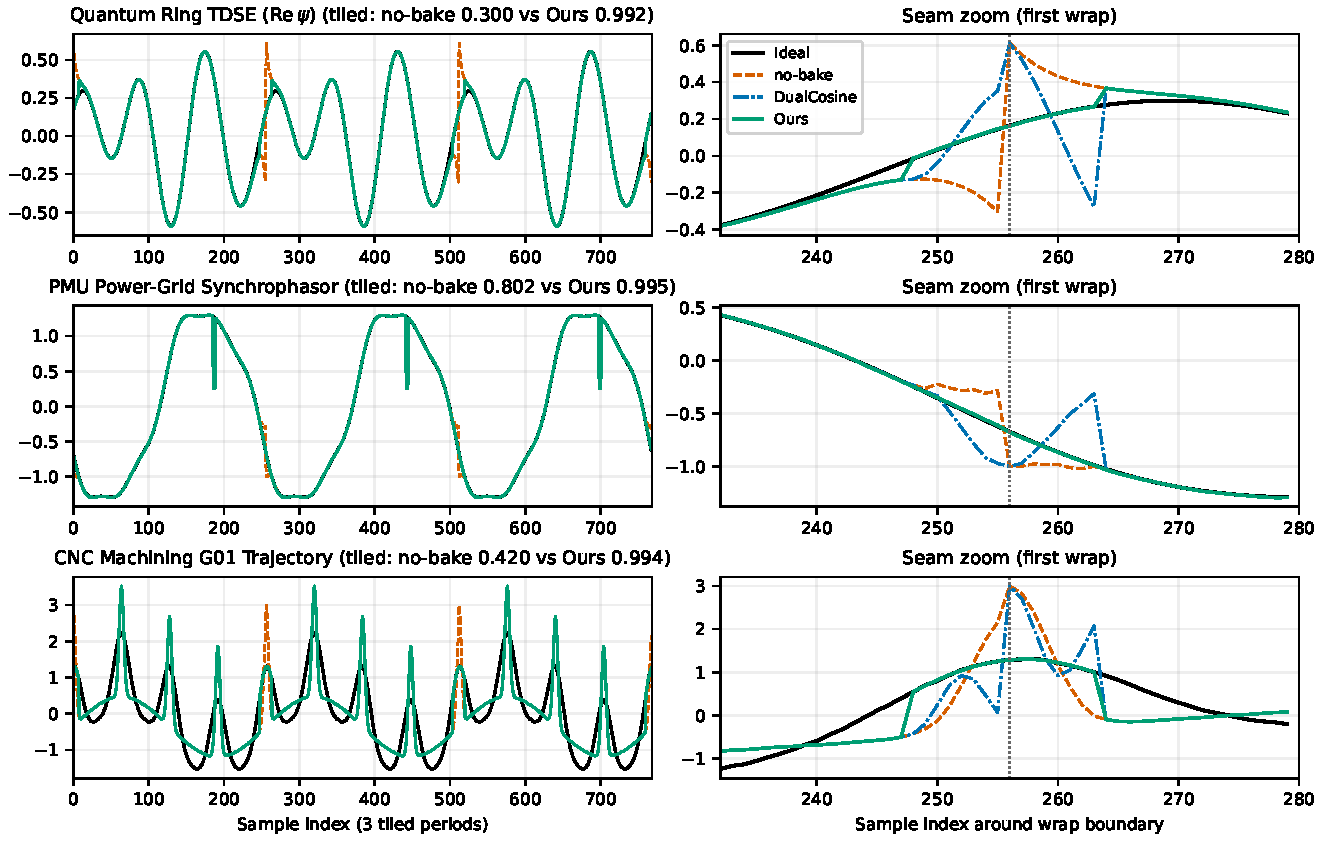
\includegraphics[width=0.95\textwidth]{figures/fig_cross_domain_quantum_samples.pdf}
  \caption{Held-out wrap-repair sample visualizations beyond audio across quantum mechanics and engineering domains: 1D periodic ring TDSE ($\mathrm{Re}\,\psi$, top), PMU power-grid synchrophasor (middle), and CNC machining G01 trajectory (bottom).
    Left: three tiled periods comparing ideal reference, \texttt{no-bake}, and FitCell-tuned \texttt{Ours}. Right: $48$-sample zoom around the first wrap boundary ($n{=}256$), where \texttt{DualCosine} introduces seam oscillations while \texttt{Ours} tracks the ideal boundary smoothly.}
  \label{fig:cross-domain-quantum-samples}
\end{figure*}

\section{Cross-domain wrap transfer}
\label{app:transfer-bundle}

Transfer boards stress the same wrap-discontinuity protocol on non-audio periodic signals.
They are not claims of bearing-fault or ECG diagnosis SOTA.
Algorithms for the residual score and hybrid loop appear in Appendix~\ref{app:algorithms}; raw cross-domain tables and figures are archived in the unified repository (\codehref{https://github.com/reeldemo/denoise-opt}{reeldemo/denoise-opt}).

% Main-text sci/eng wrap transfer (elevated from appendix-only in v9).
% Included from experiments.tex.

\subsection{Cross-domain wrap transfer protocol}
\label{sec:transfer-protocol}

The primary claim of this paper is wavetable seam repair.
Transfer boards answer a narrower mechanistic question:
does the \emph{same} wrap-discontinuity protocol (open a cliff at a period join, score against a no-cliff ideal sibling, fit a compact repair operator) still make sense on other short periodic signals?
They are stress tests of that geometry.
They are \emph{not} claims that an audio-trained bake transfers as bearing-fault or ECG diagnosis SOTA,
and they are not claims that fatigue cracks or grid phase events ``are'' wavetable seams.
Reported transfer evidence is only locked $R_{\mathrm{blend}}$ on the seven wrap boards in Table~\ref{tab:transfer-main}; I do not claim cross-domain generalization beyond that residual protocol.

\paragraph{Shared transfer recipe.}
For each domain I cut fixed-length periods ($L{=}256$) and build an ideal sibling (smooth / template / cubic path) plus a cracked engine (same content with an open-wrap cliff, sometimes with a deliberately worse interpolant).
I then score classical baselines and a domain-trained DenoiseOpt / Noise2Noise stack under locked $R_{\mathrm{blend}}$ as defined in Section~\ref{sec:residual-score}
(\texttt{hybrid\_lstm} FitCell, $150$--$250$ outer iterations where searched, short \texttt{fit\_steps}${}={}40$ on transfer boards).
Classical baselines on every board: no-bake (passthrough), DualCosine (raised-cosine end fade), \texttt{seam\_fir3}, and endpoint-pin (shared DualCosine/FIR interface; Section~\ref{sec:classical-board}).
SeamN2N: corrupt$\to$corrupt CNN, ${\approx}53.5$k params, $4000$ Adam steps, train seed \texttt{424242}.
Domain-trained Noise2Noise (corrupt$\to$corrupt, $4000$ Adam steps) is scored on the same seven boards and reported beside classical rows in Table~\ref{tab:transfer-main}.
Artifacts:
\href{https://github.com/reeldemo/denoise-opt}{signal\_heal\_transfer}.

\paragraph{Seam analogy by domain family.}
\textbf{Bearing revolutions (CWRU / MFPT / Paderborn).}
One shaft revolution is the period.
The seam is the join between the last and first angle samples after resampling to $L{=}256$.
A wrap cliff models a bad change-of-time / interpolant at that join, not a physics model of fatigue crack growth.
Ideal siblings use a smoother angular path (cubic) than the cracked engine (linear + cliff).

\textbf{ECG beats (MIT-BIH / PTB-XL subset).}
One heartbeat (R--R window) is the period.
The seam is the join between beat end and beat start when the window is tiled.
A wrap cliff is an artificial endpoint mismatch on that window.
The ideal is a mild endpoint-equalized beat template.
Clinical arrhythmia restore metrics are out of scope.

\textbf{Synthetic CNC / PMU.}
Stand-ins for closed machine-tool contours and one AC / PMU voltage cycle when real KIT / IEEE DataPort downloads are walled.
The seam is again a period-join cliff under the same residual protocol.
These rows are procedural pilots, not industrial toolpath or live-grid claims.

\paragraph{What each dataset is (pointers).}
CWRU / MFPT / Paderborn K001: public vibration, $n{=}256$ revolutions each (Paderborn also hosts a separate Al~Firdausi 4-class fault classifier, labeled apart from wrap-$R_{\mathrm{blend}}$).
MIT-BIH and PTB-XL 500\,Hz lead-I subset: PhysioNet beat windows, $n{=}256$.
Synthetic CNC G01 and synthetic PMU/AC: procedural, $n{=}256$.

\paragraph{Scope note.}
Transfer tables compare classical rows, domain-trained Noise2Noise, and Ours under this residual protocol.
Author ECG Cycle-GAN and BeatDiff carry OOD wrap probes, while Paderborn Al~Firdausi is a trained fault classifier (plus labeled arch-reuse wrap bake).
Formal listening remains out of scope (Section~\ref{sec:limitations} and Table~\ref{tab:transfer-sota-status}).
Results appear in Appendix Section~\ref{sec:transfer-main}.

\subsection{Transfer to bearings, ECG, and synthetic cycles}
\label{sec:transfer-main}

\paragraph{Setup reminder.}
Table~\ref{tab:transfer-main} reports the primary metric \textbf{locked $R_{\mathrm{blend}}$} (higher better; $\alpha{=}0.7$ seam/body blend from Section~\ref{sec:residual-score}) after training/searching DenoiseOpt
(\texttt{hybrid\_lstm}, seed \texttt{1902771841}) on each transfer board
from Section~\ref{sec:transfer-protocol} ($n{=}256$ periods, $L{=}256$).
No PESQ/STOI/MOS appears on these boards: periods are non-speech wrap tiles, and the claim is wrap-protocol residual repair only.
Columns are: CWRU/MFPT/Paderborn bearing revolutions, MIT-BIH/PTB-XL ECG beats, and synthetic CNC/PMU pilots.
Numbers come from the released
\href{https://github.com/reeldemo/denoise-opt}{cross-domain transfer summary}
(\texttt{primary\_metric=r\_blend}).
Domain-trained Noise2Noise-style SeamN2N (corrupt$\to$corrupt, $4000$ Adam steps, train seed \texttt{424242}, holdout seed \texttt{20260719})
is scored on the same seven boards under the \emph{same} $R_{\mathrm{blend}}$.
Author ECG Cycle-GAN and BeatDiff remain OOD wrap probes on ECG only
(clinical restore $\neq$ wrap residual; status notes in Appendix~\ref{app:supplement}, Table~\ref{tab:transfer-sota-status}).
These rows do \emph{not} transfer an audio-trained bake as fault/ECG diagnosis SOTA; they only stress the wrap geometry.
Artifacts:
\href{https://github.com/reeldemo/denoise-opt}{signal\_heal\_transfer}.

\begin{table}[t]
  \centering
  \caption{Wrap-heal transfer under locked $R_{\mathrm{blend}}$ (higher better; wrap-protocol stress test).
  Bearing boards ($n{=}256$ each). DenoiseOpt: \texttt{hybrid\_lstm}, seed \texttt{1902771841}.}
  \label{tab:transfer-main}
  \setlength{\tabcolsep}{3pt}
  \footnotesize
  \begin{tabular}{@{}lccc@{}}
    \toprule
    Method & CWRU & MFPT & Paderborn \\
    \midrule
    Ours & 0.960 & 0.943 & 0.937 \\
    SeamN2N & 0.866 & 0.866 & 0.842 \\
    no-bake & 0.845 & 0.866 & 0.838 \\
    endpoint-pin & 0.505 & 0.545 & 0.567 \\
    \texttt{seam\_fir3} & 0.448 & 0.573 & 0.560 \\
    DualCosine & 0.461 & 0.483 & 0.471 \\
    \bottomrule
  \end{tabular}
\end{table}

\begin{table}[t]
  \centering
  \caption{Wrap-heal transfer under locked $R_{\mathrm{blend}}$ (continued): ECG and synthetic boards.
  BeatDiff / Cycle-GAN are author OOD wrap probes on ECG only.}
  \label{tab:transfer-main-b}
  \setlength{\tabcolsep}{2.5pt}
  \footnotesize
  \begin{tabular}{@{}lcccc@{}}
    \toprule
    Method & MIT-BIH & PTB-XL & CNC & PMU \\
    \midrule
    Ours & 0.975 & 0.945 & 0.991 & 0.992 \\
    SeamN2N & 0.750 & 0.754 & 0.553 & 0.959 \\
    no-bake & 0.750 & 0.762 & 0.450 & 0.936 \\
    endpoint-pin & 0.865 & 0.870 & 0.410 & 0.944 \\
    \texttt{seam\_fir3} & 0.766 & 0.760 & 0.534 & 0.912 \\
    DualCosine & 0.414 & 0.512 & 0.494 & 0.827 \\
    BeatDiff (OOD) & 0.491 & 0.493 &, &, \\
    Cycle-GAN (OOD) & 0.106 & 0.211 &, &, \\
    \bottomrule
  \end{tabular}
\end{table}

\paragraph{Takeaways (wrap-protocol stress test; not domain SOTA).}
Under $R_{\mathrm{blend}}$, Ours has the top \emph{pointwise} score in each column of Tables~\ref{tab:transfer-main}--\ref{tab:transfer-main-b} on these seven boards (diagnostic comparison; no multi-seed inferential claim).
SeamN2N exceeds Dual Cosine on every column and sits near no-bake on several bearing / ECG columns, but trails Ours
on ECG and synth CNC.
On MIT-BIH and PTB-XL, endpoint-pin remains a strong classical ECG row above SeamN2N. Ours still leads both.
Author Operational Cycle-GAN and BeatDiff collapse under OOD wrap scoring relative to Ours / SeamN2N / no-bake.
I do not treat clinical morph metrics as wrap residual.
Synthetic CNC shows the largest classical collapse with Ours near $0.991$.
Synth PMU is the strongest SeamN2N row ($0.9589$) but still below Ours ($0.9919$).
Paderborn wrap board shows Ours $0.9369$ vs SeamN2N $0.8421$ and DualCosine $0.4710$.
Separately, I train Al~Firdausi CNN as a 4-class fault classifier and do not rename classification as wrap residual
(Appendix Table~\ref{tab:transfer-sota-status}).
Figure~\ref{fig:signal-heal-transfer-main} summarizes the same boards as grouped bars.
Latency timings in Appendix~\ref{app:supplement} remain wavetable-checkpoint zero-shot.
Primary claim remains cycle-local wavetable seam restoration.

\begin{figure}[t]
  \centering
  \includegraphics[width=\columnwidth]{figures/fig_signal_heal_transfer.png}
  \caption{Grouped bars for Tables~\ref{tab:transfer-main}--\ref{tab:transfer-main-b}: $R_{\mathrm{blend}}$ by board and method
    (higher better). Core rows (Ours, SeamN2N, no-bake, endpoint-pin, \texttt{seam\_fir3}, DualCosine)
    appear on all seven boards. Hatched bars are author OOD wrap probes on ECG (BeatDiff, Cycle-GAN)
    and the Paderborn Al~Firdausi architecture-reuse wrap bake
    (not the published fault classifier, see Table~\ref{tab:transfer-sota-status}).
    Missing cells are omitted rather than zero-filled.}
  \label{fig:signal-heal-transfer-main}
\end{figure}

\subsection{Listening protocol (no formal listening study)}
\label{sec:listening-protocol}

Downloadable WAVs
(\href{https://github.com/reeldemo/denoise-opt}{hear-sample WAVs})
and vibrato spectrograms are released for informal file inspection
(Sections~\ref{sec:vibrato-eval}--\ref{sec:hear-samples}).
They are regenerated from the same public procedural / holdout tiles used in the residual tables, not private studio stems.
Formal MOS / MUSHRA / forced-choice A/B was not run ($N_{\mathrm{listeners}}{=}0$), so I report no preference rates or significance tests.
Until a powered listening study runs, I make \emph{no} perceptual quality claim; residual $R_{\mathrm{blend}}$ is the sole primary evidence.
See Section~\ref{sec:limitations}.



\end{document}
